\begin{Soln}{2}
\begin{enumerate}
\item
Comme il y a plus d'élèves que de jours dans l'année, il y a au moins deux élèves qui fêtent leur anniversaire le même jour.

\item À partir de $367$ élèves, on peut conclure de la même manière.

\item S'il y a $2\times 366=732$ élèves, il est possible qu'exactement deux d'entre eux fêtent leur anniversaire chaque jour. À partir de $2\times 366+1=733$ élèves, il y en a forcément trois qui fêtent leur anniversaire le même jour.
\end{enumerate}
\end{Soln}
\begin{Soln}{4}
Notons $n$ le nombre de participants\footnote{Méthode : nommer les objets permet de raisonner ou de faire des calculs dessus plus clairement.}. Pour chaque entier $k$ compris entre $1$ et $n$, notons $a_n$ le nombre personnes que connaît le $n$-ème participant. Alors les $a_i$ sont $n$ entiers entre $0$ et $n-1$ et il s'agit de montrer que deux d'entre eux sont identiques. (Notons que le principe des tiroirs ne permet pas de conclure immédiatement, puisqu'il y a $n$ entiers à distribuer dans $n$ tiroirs.)

Supposons que tous les $a_i$ soient distincts\footnote{Méthode : raisonnement par l'absurde.}. Alors ils valent forcément (dans le désordre) $0$, $1$, $2$, .. $n-1$. Ceci signifie qu'un participant connaît tout le monde, et qu'un autre ne connaît personne, ce qui est absurde. On en déduit que deux des entiers $a_i$ sont égaux.
\end{Soln}
\begin{Soln}{5}
\begin{enumerate}
\item On pose la division. Au bout d'un certain temps, on n'abaisse plus que des zéros, et les restes sont tous strictement inférieurs au diviseur (le dénominateur de la fraction). De plus, chaque reste détermine de façon déterministe toute la suite du développement décimal. Donc soit le développement décimal est fini, soit il y a une infinité de chiffres après la virgule, donc une infinité de restes, or les valeurs de ces restes sont en nombre fini. Il existe donc deux restes égaux. Comme ils déterminent la suite du développement, on en déduit que le développement est périodique, et que la période est de longueur inférieure au dénominateur.
\item Notons $x=a_k...a_1a_0,b_1b_2...b_l\overline{b_{l+1}b_{l+2}...b_{l+m}}$ un développement décimal illimité périodique à partir du rang $l+1$, avec une période égale à $m$. On note enfin $p$ le nombre s'écrivant $b_{l+1}b_{l+2}...b_{l+m}$.

Alors $10^{l+m}x - 10^lx$ est un entier, noté $p$, d'où $x = \frac{p}{10^{l+m} - 10^l} = \frac{p}{10^l(10^m-1)}$
\item Pour le nombre $x=0,131313...$, avec les notations plus haut, $l=0$, $m=2$, $p=13$, et le raisonnement plus haut dans ce cas particulier est que $100x-x=13$, et donc que $x=\frac{13}{99}$.

Si $x=0,345345345...$, le raisonnement précédent donne $x=\frac{345}{999}$, et si $x=1,4666666$, on obtient $x=\frac{146-14}{100-10}=\frac{132}{90}$.

Pour finir, si $x=1,234565656...$, on a $(10^5-10^3)x=123456-1234=122222$, d'où on déduit que $x=\frac{122222}{99000}$.
\end{enumerate}
\end{Soln}
\begin{Soln}{6}
Comme chaque coefficient est compris entre $-1$ et $1$, la somme de trois coefficients est comprise entre $-3$ et $3$, ce qui fait sept valeurs entières possibles.

D'autre part il y a huit sommes à calculer (les trois lignes, les trois colonnes et les deux diagonales).

Donc par le principe des tiroirs, au moins deux sommes sont identiques.
\end{Soln}
\begin{Soln}{7}


Notons les points $A$, $B$ $C$ et $D$, dans l'ordre d'apparition sur le cercle trigonométrique dans le sens direct. Notons également $\alpha$, $\beta$, $\gamma$ et $\delta$ les quatre angles formés par les points : par exemple $\alpha = \widehat{AOB}$, $\beta = \widehat{BOC}$ etc.

\begin{center}\definecolor{qqwuqq}{rgb}{0.,0.39215686274509803,0.}
\definecolor{uuuuuu}{rgb}{0.26666666666666666,0.26666666666666666,0.26666666666666666}
\definecolor{xdxdff}{rgb}{0.49019607843137253,0.49019607843137253,1.}
\definecolor{qqqqff}{rgb}{0.,0.,1.}
\begin{tikzpicture}[line cap=round,line join=round,>=triangle 45,x=1.0cm,y=1.0cm]
\clip(-1.9,-1.58) rectangle (4.12,4.88);
\draw [shift={(0.6740732265446223,1.9791533180778031)},color=qqwuqq,fill=qqwuqq,fill opacity=0.10000000149011612] (0,0) -- (26.942256799284916:0.7) arc (26.942256799284916:133.55289331740752:0.7) -- cycle;
\draw [shift={(0.6740732265446223,1.9791533180778031)},color=qqwuqq,fill=qqwuqq,fill opacity=0.10000000149011612] (0,0) -- (133.55289331740752:0.6) arc (133.55289331740752:242.70731139090447:0.6) -- cycle;
\draw [shift={(0.6740732265446223,1.9791533180778031)},color=qqwuqq,fill=qqwuqq,fill opacity=0.10000000149011612] (0,0) -- (-117.29268860909559:0.7) arc (-117.29268860909559:-23.247011961144597:0.7) -- cycle;
\draw [shift={(0.6740732265446223,1.9791533180778031)},color=qqwuqq,fill=qqwuqq,fill opacity=0.10000000149011612] (0,0) -- (-23.24701196114459:0.6) arc (-23.24701196114459:26.942256799284912:0.6) -- cycle;
\draw(0.6740732265446223,1.9791533180778031) circle (2.4296300551874013cm);
\draw (0.6740732265446223,1.9791533180778031)-- (-1.,3.74);
\draw (0.6740732265446223,1.9791533180778031)-- (-0.44,-0.18);
\draw (0.6740732265446223,1.9791533180778031)-- (2.906445979301415,1.0201881999327287);
\draw (0.6740732265446223,1.9791533180778031)-- (2.84,3.08);
\draw [shift={(0.6740732265446223,1.9791533180778031)},color=qqwuqq] (133.55289331740752:0.6) arc (133.55289331740752:242.70731139090447:0.6);
\draw[color=qqwuqq] (0.13950049996759253,1.902785785709656) -- (0.02070656072825245,1.885815222961179);
\draw [shift={(0.6740732265446223,1.9791533180778031)},color=qqwuqq] (-117.29268860909559:0.7) arc (-117.29268860909559:-23.247011961144597:0.7);
\draw[color=qqwuqq] (0.8901312263098695,1.376725778254597) -- (0.9306421012658533,1.2637706145377454);
\draw[color=qqwuqq] (0.8096502473089637,1.3536784013619803) -- (0.8350709387022781,1.2364018544777637);
\draw[color=qqwuqq] (0.9669153930321975,1.4100808573780572) -- (1.0218232992486171,1.3033797709968553);
\draw [shift={(0.6740732265446223,1.9791533180778031)},color=qqwuqq] (-23.24701196114459:0.6) arc (-23.24701196114459:26.942256799284912:0.6);
\draw[color=qqwuqq] (1.2137924845951293,1.996563731324211) -- (1.333730097495242,2.000432712045635);
\draw[color=qqwuqq] (1.2124628314461892,1.9374803852084292) -- (1.3321049658687591,1.9282197334596796);
\draw[color=qqwuqq] (1.208657704440154,2.0554385459608104) -- (1.3274542550836053,2.0723908188237004);
\begin{scriptsize}
\draw [fill=qqqqff] (2.84,3.08) circle (2.5pt);
\draw[color=qqqqff] (2.98,3.45) node {$A$};
\draw [fill=qqqqff] (-1.,3.74) circle (2.5pt);
\draw[color=qqqqff] (-0.86,4.11) node {$B$};
\draw [fill=qqqqff] (-0.44,-0.18) circle (2.5pt);
\draw[color=qqqqff] (-0.64,-0.53) node {$C$};
\draw [fill=xdxdff] (2.906445979301415,1.0201881999327287) circle (2.5pt);
\draw[color=xdxdff] (3.26,1.05) node {$D$};
\draw [fill=uuuuuu] (0.6740732265446223,1.9791533180778031) circle (1.5pt);
\draw[color=qqwuqq] (1.12,3.09) node {$\alpha$};
\draw[color=qqwuqq] (-0.04,2.01) node {$\beta$};
\draw[color=qqwuqq] (1.24,1.05) node {$\gamma$};
\draw[color=qqwuqq] (1.88,2.07) node {$\delta$};
\end{scriptsize}
\end{tikzpicture}
\end{center}

Montrons pour commencer qu'un de ces angles est inférieur à $\pi/2$.

Le plus petit des quatre angles est inférieur ou égal à leur moyenne, et cette moyenne vaut $m=\frac{\alpha+\beta+\gamma+\delta}{4} = \frac{2\pi}{4} =  \frac{\pi}{2}$.

On vérifie alors que la distance entre les deux points formant cet angle est inférieure à $\sqrt2$.
\end{Soln}
\begin{Soln}{8}

On écrit l'ensemble $\{1,2,...,2n\}$ comme la réunion disjointe des $n$ parties suivantes
\[ \{1,2,...,2n\} = \{1,2 \} \cup \{3,4 \}\cup ... \cup \{2n-1,2n \}.\]
Si on a $n+1$ entiers, alors il y a un des \og tiroirs\fg{} contient deux entiers, ce qui signifie que deux des entiers sont consécutifs.\\

\emph{Deuxième solution, sans utiliser le principe des tiroirs}: on va considérer les différences entre les entiers. Ce sont des entiers strictement positifs (la différence vaut $1$ ssi les deux entiers sont consécutifs).

La somme de toutes ces différences est aussi la différence entre le premier et le dernier. Elle est donc inférieure à $2n-1$.

D'autre part, il y a $n+1$ entiers, donc $n$ différences. S'il n'y a pas d'entiers consécutifs, alors toutes ces différences valent au moins deux, et comme il y en a $n$, la somme des différences vaut au moins $2n$. Contradiction !

\emph{Exercice d'approfondissement : chercher le nombre de parties de $\{1, ..., n\}$ sans éléments consécutifs.}
\end{Soln}
\begin{Soln}{9}
 La solution qui suit n'est pas rédigée sous forme compacte, au contraire on explique les étapes du raisonnement.

On va appliquer le principe des tiroirs, autrement dit on va partager le carré en un certain nombre de parties, les tiroirs, qui devront vérifier les propriétés suivantes:
\begin{enumerate}
\item il y a suffisamment  de tiroirs pour que l'on puisse conclure par le principe des tiroirs qu'il existe trois points dans le même tiroir;
\item si deux points sont dans le même tiroir, alors la distance entre les points est $\leq 2/7$.
\end{enumerate}

Commençons déjà par déterminer le nombre de tiroirs nécessaire pour faire marcher le raisonnement.

Si le nombre $n$ de tiroirs est égal ou supérieur à $51/2$, on aura donc $51 \leq 2n$ donc il sera possible de répartir les points dans les tiroirs de façon à ce qu'un tiroir ne contienne pas plus de deux points. Par contre, si $n$ est strictement inférieur à $51/2$, on aura $51> 2n$, ce qui signifie bien que si l'on met deux points par tiroir, il reste encore au moins un point : il existe donc (au moins) un tiroir qui contient (au moins) trois points.

Comme $\frac{51}{2} = 25,5$ on voit que pour faire le raisonnement, il ne faut pas plus de $25$ tiroirs.

Ensuite, il faut définir précisément ces tiroirs de telle manière que deux points dans le même tiroir soient toujours à distance $\leq \frac{2}{7}$. Les tiroirs doivent donc être assez petits pour cela, on va donc essayer avec le nombre maximal de tiroirs, c'est-à-dire $25$.

Comment partager un carré en $25$ parties ? Le plus simple est de le partager en $25$ carrés plus petits, en subdivisant les côtés par cinq. Voyons si cette construction fonctionne.

Les $25$ petits carrés ont alors un côté égal à $\frac15$. Deux points dans un tel carré sont distants d'au plus la la diagonale du carré, qui mesure par Pythagore $\sqrt{\left(\frac{1}{5}\right)^2+\left(\frac{1}{5}\right)^2} = \sqrt{\frac{2}{25}} = \frac{\sqrt 2}{5}$. Il reste donc à vérifier que cette quantité est inférieure à $\frac27$, c'est-à-dire à vérifier que $\frac{\sqrt 2}{5} \leq \frac27$.

Or, cette inégalité est équivalente, en multipliant des deux côtés par $5$, à $\sqrt 2 \leq \frac{10}{7}$. Comme les deux membres de cette inégalité sont positifs, elle est équivalente à l'inégalité obtenue en élevant les deux membres au carré, autrement dit $2\leq \frac{100}{49}$. Et effectivement, on a bien $2\times 49 \leq 100$. L'inégalité est donc vraie. En remontant le raisonnement, cela signifie bien que la diagonale d'un carré de côté $\frac15$ est plus petite que $\frac27$.
\end{Soln}
\begin{Soln}{10}
Notons $(x_1,y_1)$, ..., $(x_5,y_5)$ les cinq points, repérés par leurs coordonnées qui sont des nombres entiers.

À chaque point, on associe la parité (notée $0$ ou $1$) de chacune de ses deux coordonnées. Il y a donc quatre choix possibles pour les parités de $(x,y)$, à savoir $(0,0)$ (abscisse et ordonnée paires), $(0,1)$ (abscisse paire et ordonnée impaire), $(1,0)$ et $(1,1)$.

Comme il y a cinq points et quatre choix (quatre \og tiroirs\fg), il y a forcément deux points $(x,y)$ et $(x',y')$ dont les abscisses et les ordonnées ont même parité. Leur milieu a pour coordonnées $\left(\frac{x+x'}{2},\: \frac{y+y'}{2}\right)$, et il est donc à coordonnées entières, puisque la somme de deux nombres de même parité est multiple de deux.
\end{Soln}
\begin{Soln}{11}
On veut appliquer le principe des tiroirs, la conclusion devant être qu'il existe deux points dans le même tiroir. Pour cela, il faut au plus cinq tiroirs, puisqu'il y a six points.

D'autre part, le diamètre (c'est-à-dire la distance maximale entre deux points) de ces tiroirs doit être inférieur ou égal à $\sqrt 5$.

(Insérer figure.)% Attention !
\end{Soln}
\begin{Soln}{12}
Partageons le triangle équilatéral en quatre sous-triangles équilatéraux de côté $1$, obtenus en reliant les milieux des côtés entre eux.

Par le principe des tiroirs, il existe deux points dans le même petit triangle. Deux tels points sont forcément à une distance inférieure à un l'un de l'autre.
\end{Soln}
\begin{Soln}{13}

Tout nombre s'écrit de manière unique sous la forme $i \cdot 2^k$, avec $i$ un ombre impair.

Il y a $n$ nombres impairs entre $1$ et $2n$. Par le principe des tiroirs, deux des nombres ont une décomposition avec le même nombre impair. L'un s'écrit donc $i\cdot 2^k$, et l'autre, $i\cdot 2^l$, avec le même nombre impair $i$. On en déduit que l'un est multiple de l'autre, par un facteur qui est puissance de deux, ce qui est plus fort que ce qui était demandé.\\

\emph{Cette solution est difficile à trouver : il faut avoir l'idée de la forme, pour associer un entier à un entier. Il existe d'autres solutions plus pédestres, par exemple la suivante.\\
L'exercice comporte un paramètre : $n$. Méthodologie de base : essayer avec de petites valeurs de $n$ pour voir ce qu'il se passe.  Essayer aussi avec la plus petite valeur possible de $n$.\\
Le plus petit entier autorisé est $1$. Dans ce cas, il y a deux entiers entre $1$ et $2$, et on a bien $1|2$. Ca marche mais ça n'apprend pas grand chose.\\
Essayons avec $n=3$ : on a quatre entiers entre $3$ et $6$. On voit effectivement que ça marche.\\
On suit alors un raisonnement par l'absurde. Supposons qu'une partie $A$ de cardinal $n+1$ ne contienne pas de paire dont un élément divise l'autre.\\
Comme $A$ contient  $n+1$ entiers, il y en a un entre $1$ et $n$. Notons-le $a_1$. Alors, il en existe un multiple $b_1$ entre $n+1$ et $2n$.\\
Or il reste $n$ entiers à déterminer dans $A$, et l'entier $b_1$ est exclu. Il y en a donc un autre inférieur ou égal à $n$. Notons-le $a_2$. Il admet lui aussi un multiple $b_2$ entre $n+1$ et $2n$. En itérant ce raisonnement, on finit par montrer que $1\in A$, contradiction.}
\end{Soln}
\begin{Soln}{14}
\emph{(Point méthode : si on veut utiliser le principe des tiroirs, il semble qu'il faille au plus onze \og tiroirs\fg, puisqu'il y a douze entiers.)}


Les nombres à deux chiffres identiques sont exactement les multiples de onze.

Soit $\phi$ l'application qui à chacun des douze entiers de l'énoncé associe son reste modulo onze, c'est-à-dire le reste dans la division euclidienne par onze. Il y a onze restes possibles, et douze entiers, donc par le principe des tiroirs, deux entiers ont même reste modulo onze.

Ceci signifie exactement que leur différence est divisible par onze.


\end{Soln}
\begin{Soln}{15}
Il y a $2^{10}$ sous-ensembles possibles (en comptant l'ensemble au complet et le sous-ensemble vide bien sûr). D'autre part, les entiers sont inférieurs à $99$, donc lorsqu'on choisit certains entiers et qu'on les somme, le résultat est (positif et) inférieur à $990$. Par le principe des tiroirs, il existe deux sous-ensembles différents qui ont la même somme.

Ces sous-ensembles peuvent avoir des entiers en commun, mais on voit alors qu'il suffit d'enlever ces entiers des deux sous-ensembles, et les deux sommes restent égales.
\end{Soln}
\begin{Soln}{16}
Procédons par l'absurde.

Considérons les quatre restes modulo cinq de ces entiers. Ils sont tous différents car si deux restes sont égaux, la différence des entiers en question est divisible par cinq.

Il suffit alors de les restes pour voir qu'au moins une somme est multiple de cinq.
\end{Soln}
\begin{Soln}{17}
Les sept restes modulo $10$ sont tous distincts. On voit qu'avec six entiers, les restes pourrait être $0$, $1$, $2$, ... $5$, mais qu'avec sept entiers, il y a au moins deux restes dont la somme est $10$.
\end{Soln}
\begin{Soln}{18}
Montrons d'abord que le produit est divisible par trois.
On considère les restes modulo trois des six différences, sachant que trois différences déterminent les trois autres. Il y a trois restes possibles : si l'un est nul  c'est bon, sinon par le principe des tiroirs, il y a deux restes égaux. Dans ce cas on montre qu'une des trois autres différences est divisible par trois.

Par la divisibilité par quatre, on montre que deux différences sont paires.

\end{Soln}
\begin{Soln}{19}
Notons $n_1, \ldots, n_101$ la suite d'entiers obtenue. Pour chaque indice $i$ compris entre $1$ et $101$, on note $a_i$ la longueur de la plus longue sous-suite croissante qui se termine par $n_i$ et $b_i$ la longueur de la plus longue sous-suite d\'ecroissante qui se termine par $n_i$. Ainsi, on a associ\'e un couple d'entiers \`a chacun des termes de la suite.\newline

D'une part, on voit que tous ces couples sont distincts. En effet, soient $i<j$, on est toujours dans l'un des deux cas suivants:
\begin{itemize}
\item soit $n_i<n_j$ auquel cas on a forc\'ement $a_i<a_j$,
\item soit $n_i>n_j$ et dans ce cas $b_i<b_j$.
\end{itemize}

D'autre part, il n'y a que $\left(11-1\right)\left(11-1\right)$ couples d'entiers $\left(a,b\right)$ tels que $a,b<11$. Ainsi, parmi les $101$ couples $\left(a_i,b_i\right)$ au moins l'un d'entre eux \`a une coordonn\'ee sup\'erieure ou \'egale \`a $11$. (Th\'eor\`eme d'Erd\"os-Szekeres)
\end{Soln}
\begin{Soln}{20}
Notons $a_1$, ... $a_n$ les entiers, et considérons les sommes $S_1 = a_1$, $S_2 = a_1+a_2$, ..., $S_n = a_1+a_2+...+a_n$. Si l'une de ces sommes est divisible par $n$ (autrement dit le reste de la division par $n$ est nul, c'est terminé. Sinon, cela signifie que les restes par division par $n$ sont tous non nuls, donc doivent valoir $1$, ..., $n-1$. Or, il y a $n$ tels restes donc deux des sommes ont le même reste.

Ceci signifie alors que la différence de ces deux sommes est divisible par $n$. Or, la différence de deux des sommes est aussi une somme d'entiers de la collection.
\end{Soln}
\begin{Soln}{21}
\begin{enumerate}
\item
Dans le triangle $ABC$, en notant $I$ est le milieu de $[AB]$ et $J$ le milieu de $[BC]$, le théorème de Thalès dit que $(IJ)$ est parall\`ele \`a $(AC)$ et $IJ = \frac{1}{2} AC$. On raisonne pareillement avec le triangle $ACD$, ce qui donne $(KL)$ parall\`ele \`a $AC$ et $KL = \frac{1}{2} AC$. Or, un quadrilat\`ere qui a deux c\^ot\'es parall\`eles et de m\^eme longueur est un parall\'elogramme.

\item La preuve la plus élémentaire utilise uniquement qu'une médiane d'un triangle donné le partage en deux triangles de même aire.

Soit $O$ le point d'intersection des diagonales du quadrilat\`ere $ABCD$. On consid\`ere le triangle $AOB$. Soit $O_1$ le point d'intersection de la diagonale $[AC]$ avec $[IL]$ et soit $O_2$ le point d'intersection de $[IJ]$ avec la diagonale $[BD]$.

% Par construction, le quadrilat\`ere $IO_1OO_2$ est un parall\'elogramme.

Par le théorème de Thalès,  $O_1$ est le milieu de $[AO]$ et $O_2$ le milieu de $[BO]$. Les triangles $IO_1A$ et $IO_1B$ ont même aire, de même que les triangles $I0_2O$ et $IO_2B$.

La somme des aires des triangles $AIO_1$ et $IO_2B$ est donc exactement \'egale \`a l'aire du parall\'elogramme $IO_1OO_2$.

On applique le m\^eme raisonnement aux triangles $BCO$, $CDO$ et $ADO$, ce qui signifie que, dans le quadrilat\`ere $ABCD$, la partie compl\'ementaire de $IJKL$ a une aire qui est exactement \'egale \`a celle de $IJKL$, ce qui permet de conclure. \end{enumerate}

\end{Soln}
\begin{Soln}{22}
\underline{Première solution} : soit $\sigma$ la symétrie centrale de centre $I$ et  $A''$ (respectivement $B''$) l'image de $A'$ (resp. $B'$) par $\sigma$.

Par construction, $A'B'A''B''$ est un parallélogramme de centre $I$, et par construction également, on a $B=\sigma(A)$.

Montrons que $A'B'A''B''$ est un rectangle. Comme une symétrie centrale envoie une droite sur une droite parallèle, l'image de la droite $(AA')$ lui est parallèle, et doit forcément contenir $\sigma(A)$ c'est-à-dire $B$. C'est donc la droite $(BB')$. Ceci montre que $A''$ est le point d'intersection des droites $(A'I)$ et $(BB')$, et donc que $A'B'A''B''$ est un rectangle.

Comme les diagonales d'un rectangle on même longueur, on a terminé.

\underline{Deuxième solution} : une projection orthogonale sur une droite préserve les milieux : on peut par exemple le prouver en considérant un repère orthonormé et des coordonnées. On voit alors que la  projection orthogonale $I'$ de $I$ sur $(A'B')$ est le milieu de $[A'B']$. Ceci signifie que dans le triangle $A'IB'$, la hauteur issue de $I$ est également la médiane issue de $I$. Le triangle $A'IB'$ est donc isocèle, d'où $A'I = B'I$.
\end{Soln}
\begin{Soln}{23}
Pour montrer que $H$ est l'orthocentre du triangle $DMN$, il suffit de montrer que  $(AN)$ et $(CM)$ sont des hauteurs de ce triangle : leur point d'intersection $H$ sera alors l'orthocentre.\\

Soit $\rho$ la rotation de centre $O$ (le centre du carré) et d'angle $\pi/2$. Par définition d'un carré direct, on a $\rho(A)=B$, $\rho(B)=C$, $\rho(C)=D$ et $\rho(D)=A$.

On a de plus \underline{$\rho(M)=N$}. En effet, comme $M \in [AB]$, on a $\rho(M) \in [\rho(A)\rho(B)] = [BC]$, et d'autre part, comme $\rho$ est une isométrie, on a $AM = \rho(A)\rho(M) =  B\rho(M)$. Or il n'y a qu'un point sur $[BC]$ à distance $AM$ de $B$, et d'après l'énoncé c'est $N$.

La rotation $\rho$ envoie donc le triangle $DAM$ sur $ABN$. Comme c'est une rotation d'angle $\pi/2$, on en déduit que $(DM)\bot (AN)$ et donc que $(AN)$ est une hauteur de $DMN$. On procède de même pour la deuxième hauteur.

\emph{Remarque: on peut rédiger la solution sans rotations, juste en utilisant des angles complémentaires, mais c'est plus laborieux et moins éclairant, donc (fortement) déconseillé.}
\end{Soln}
\begin{Soln}{24}
\'Ecrire chacune des distances à l'aide d'aires de triangles. Ou bien dessiner les trois petits triangles, chaque distance est une hauteur d'un petit triangle équilatéral, faire tourner ces hauteurs.
\end{Soln}
\begin{Soln}{25}
Deuxième indication: un des angles du triangle a une mesure $\geq \pi/3$, et un autre a une mesure $\leq \pi/3$.
\end{Soln}
\begin{Soln}{27}

\begin{center}
\definecolor{qqwuqq}{rgb}{0.,0.39215686274509803,0.}
\definecolor{xdxdff}{rgb}{0.49019607843137253,0.49019607843137253,1.}
\definecolor{uuuuuu}{rgb}{0.26666666666666666,0.26666666666666666,0.26666666666666666}
\definecolor{qqqqff}{rgb}{0.,0.,1.}
\begin{tikzpicture}[line cap=round,line join=round,>=triangle 45,x=1.0cm,y=1.0cm]
\clip(-3.6,-1.06) rectangle (4.3,4.2);
\draw [shift={(1.1,3.42)},color=qqwuqq,fill=qqwuqq,fill opacity=0.1] (0,0) -- (-157.7619672844355:0.6) arc (-157.7619672844355:-107.95975501222517:0.6) -- cycle;
\draw [shift={(1.1,3.42)},color=qqwuqq,fill=qqwuqq,fill opacity=0.1] (0,0) -- (-107.95975501222517:0.6) arc (-107.95975501222517:-58.15754274001482:0.6) -- cycle;
\draw (-2.96,1.76)-- (1.1,3.42);
\draw (2.257061141239912,1.556935450545904)-- (1.1,3.42);
\draw (2.257061141239912,1.556935450545904)-- (-2.96,1.76);
\draw [dash pattern=on 5pt off 5pt] (-0.93,2.59)-- (3.414122282479824,-0.30612909890819173);
\draw [dash pattern=on 5pt off 5pt] (2.257061141239912,1.556935450545904)-- (3.414122282479824,-0.30612909890819173);
\draw [dash pattern=on 5pt off 5pt] (3.414122282479824,-0.30612909890819173)-- (-2.96,1.76);
\draw (1.1,3.42)-- (0.5180407608266075,1.6246236336972695);
\begin{scriptsize}
\draw [fill=qqqqff] (-2.96,1.76) circle (2.5pt);
\draw[color=qqqqff] (-2.82,2.12) node {$A$};
\draw [fill=qqqqff] (1.1,3.42) circle (2.5pt);
\draw[color=qqqqff] (1.24,3.78) node {$B$};
\draw [fill=uuuuuu] (-0.93,2.59) circle (1.5pt);
\draw[color=uuuuuu] (-1.32,2.92) node {$I$};
\draw [fill=xdxdff] (2.257061141239912,1.556935450545904) circle (2.5pt);
\draw[color=xdxdff] (2.4,1.92) node {$C$};
\draw [fill=qqqqff] (3.414122282479824,-0.30612909890819173) circle (2.5pt);
\draw[color=qqqqff] (3.56,0.06) node {$D$};
\draw [fill=uuuuuu] (0.5180407608266075,1.6246236336972695) circle (1.5pt);
\draw[color=uuuuuu] (0.08,1.3) node {$M$};
\end{scriptsize}
\end{tikzpicture}
\end{center}
Soit $D$ le symétrique de $C$ par rapport à $A$. Alors $[AC]$ est une médiane de $ABD$ et $M$ est son centre de gravité. En notant $I$ le milieu de $[AB]$, on voit que $IBCM$ est un cerf-volant et les angles considérés par l'énoncé sont égaux.
\end{Soln}
\begin{Soln}{28}


\begin{center}
\begin{tikzpicture}[line cap=round,line join=round,>=triangle 45,x=1.0cm,y=1.0cm]
\clip(-3.94,-0.88) rectangle (5.24,4.22);
\draw(0.47,1.75) circle (1.7800280896660026cm);
\draw [dash pattern=on 5pt off 5pt] (-0.79572113832392,0.49842099729981115)-- (-0.7815790027001891,3.0157211383239195);
\draw [dash pattern=on 5pt off 5pt] (-0.7815790027001891,3.0157211383239195)-- (1.7357211383239195,3.0015790027001885);
\draw [dash pattern=on 5pt off 5pt] (1.7357211383239195,3.0015790027001885)-- (1.7215790027001878,0.4842788616760799);
\draw [dash pattern=on 5pt off 5pt] (1.7215790027001878,0.4842788616760799)-- (-0.79572113832392,0.49842099729981115);
\draw (-1.32,-0.02)-- (-1.3,3.54);
\draw (-1.3,3.54)-- (2.26,3.52);
\draw (2.26,3.52)-- (2.24,-0.04);
\draw (2.24,-0.04)-- (-1.32,-0.02);
\draw (-1.31,1.76)-- (0.48,3.53);
\draw (0.48,3.53)-- (2.25,1.74);
\draw (2.25,1.74)-- (0.46,-0.03);
\draw (-1.31,1.76)-- (0.46,-0.03);
\end{tikzpicture}
\end{center}
\end{Soln}
\begin{Soln}{29}
Soit $\phi$ l'application du segment $[AB]$ dans lui-même qui a un point $D$ sur le segment associe le point $G$ comme construit dans l'énoncé. On veut montrer qu'appliquer deux fois de suite la fonction $\phi$ à un point revient à ne rien faire.

Pour comprendre l'application $\phi$, calculons les images de quelques points.
SI $D=A$, on voit on effectuant les trois projections que $\phi(A)=B$. On voit de la même manière que $\phi(B)=A$. L'application $\phi$ échange donc les deux extrémités du segment. D'autre part, on voit en utilisant le théorème des milieux trois fois de suite que l'image du milieu de $[AB]$ par $\phi$ est toujours le milieu de $[AB]$. Ceci porte à croire que l'application $\phi$ est la symétrie du segment par rapport à son milieu, autrement dit que si $D$ est un point de $[AB]$, alors $\phi(D)$ (autrement dit $G$ dans les notations de l'énoncé) est le point qui est à la même distance de $B$ que $D$ de $A$.

Autrement dit, on veut montrer:
\[ AD=BG\text{ ou bien, de façon équivalente: } BD =AG.\]
On prouve cette égalité en appliquant trois fois le théorème de Thalès (une fois pour chaque projection).
\end{Soln}
\begin{Soln}{30}
\begin{center}
\fbox{
\begin{minipage}{.9\linewidth}
Dire qu'un entier relatif $n$ est divisible par un entier non nul $d$ (ou de façon équivalente, dire que $n$ est un multiple de $d$), c'est dire qu'il existe $k\in \Z$ tel que $n=dk$.

(Par exemple, dire qu'un entier $n$ est pair signifie qu'il existe $k\in \Z$ tel que $n=2k$.)

Pour démontrer qu'un entier est divisible par $d$, il s'agit donc de trouver un tel $k$ qui convient. Par exemple, pour démontrer que $126$ est divisible par $7$, il suffit de remarquer qu'en posant $k=18$, on a bien $126=7k$. Trouver le nombre $k$ qui convient n'est pas forcément immédiat et il existe des méthodes pour cela (non nécessaires ici).
\end{minipage}
}
\end{center}

\begin{enumerate}
\item Le calcul des premières valeurs et l'indication poussent à essayer de montrer par récurrence que les entiers sont divisibles par trois. Pour tout $n\in \N$, on note $A(n)$ l'assertion \og $4^n-1$ est divisible par trois.\fg

\textbf{Initialisation.} L'assertion $A(0)$ est \og $4^0-1$ est divisible par trois\fg. Elle est donc vraie, car $4^0-1=0$, et $0$ est bien divisible par trois : on peut écrire $0=3k$, avec $k=0$.

\textbf{Hérédité.} Soit $n\in \N$ et supposons que $A(n)$ soit vraie, c'est-à-dire que $4^n-1$ soit divisible par trois. Ceci signifie par définition qu'il existe un entier relatif $k$ tel que $4^n-1=3k$.

Prouvons maintenant l'assertion $A(n+1)$, c'est-à-dire prouvons que $4^{n+1}-1$ est divisible par trois.

On a
\begin{align*}
4^{n+1}-1 &= 4\cdot 4^n - 1\\
		  &= (3+1)\cdot 4^n - 1\\
		  &= 3\cdot 4^n + (4^n-1)\\
		  &= 3(4^n+k).
\end{align*}
Donc $A(n+1)$ est vraie.\\
\textbf{Conclusion.} D'après le principe de récurrence, on a montré que pour tout $n\in \N$, $A(n)$ est vraie.\\



Essayons maintenant de généraliser le résultat. Dans l'expression $4^n-1$, les valeurs arbitraires que l'on pourrait être amené à changer son $4$ et $1$. Expérimentons, par exemple étudions les nombres du type $5^n-1$. Les premières valeurs sont $0$, $4$, $5^2-1=24$, $125-1=124$, qui sont tous divisibles par quatre.

Ceci mène à conjecturer la véracité de l'assertion suivante : \og Si $a\geq 2$ est un entier, $a^n-1$ est divisible par $a-1$.\fg

On peut prouver ce résultat par récurrence, la preuve étant identique à celle pour $a=4$: Pour l'hérédité, on écrit:
\[ a^{n+1}-1 = a\cdot a^n-1 = (a-1+1)a^n-1= (a-1)a^n + a^n-1.\]

\item On montre de même que les $8^n-3^n$ sont divisibles par cinq. En fait on peut là aussi généraliser et montrer que si $a$ et $b$ sont des entiers distincts, alors pour tout $n\in \N$, $a^n-b^n$ est divisible par $a-b$.

\textbf{Initialisation.} L'assertion $A(0)$ est \og $a^0-b^0$ est divisible par $a-b$\fg, c'est-à-dire \og $0$ est divisible par $a-b$\fg. Elle est donc vraie.

\textbf{Hérédité.} Soit $n\in \N$ et supposons que $A(n)$ soit vraie, c'est-à-dire que $a^n-b^n$ soit divisible par $a-b$. Par définition, cela signifie qu'il existe $k\in\Z$ tel que $a^n-b^n=(a-b)k$.

Prouvons maintenant l'assertion $A(n+1)$, c'est-à-dire prouvons que $a^{n+1}-b^{n+1}$ est divisible par $a-b$.

On a
\begin{align*}
a^{n+1}-b^{n+1} &= (a-b+b)a^n-b\cdot b^n\\
		  &= (a-b)a^n + b(a^n-b^n)\\
		  &= (a-b)a^n + b(a-b)k\\
		  &= (a-b)(a^n+bk).
\end{align*}
Donc $A(n+1)$ est vraie.\\
\textbf{Conclusion.} Par le principe de récurrence, on a bien montré que pour tout $n\in \N$, $a-b$ divise $a^{n}-b^{n}$.

\end{enumerate}

Terminons par deux remarques:
\begin{enumerate}
\item Si on connaît les congruences, on peut facilement montrer ces résultats sans utiliser de récurrence, juste en calculant avec des congruences, par exemple de la façon suivante:
\[
4\equiv 1 ~[3]
\Rightarrow 4^n\equiv 1^n~[3]
\Leftrightarrow 4^n-1\equiv 0~[3]
\Leftrightarrow 3 | 4^n-1.
\]
(Exercice : rédiger la preuve pour $a-b | a^n-b^n$.)\\
(Attention ! La première implication n'est pas une équivalence : on peut multiplier des congruences de nombres entiers mais cela ne donne pas des congruences équivalentes, de la même façon que l'on peut multiplier des égalités mais cela ne donne pas des égalité équivalentes : par exemple si on a $x=-2$, on peut prendre le carré terme a terme ce qui donne $x^2=4$ et est correct, mais ce n'est pas équivalent : si $x^2=4$, on n'a pas forcément $x=-2$)

\item En fait, il n'y a même pas besoin de congruences, car tout découle de deux identités remarquables. La première question doit faire penser à la formule de la série géométrique : la raison pour laquelle $a^n-1$ est un multiple de $a-1$ est simplement que l'autre facteur est $a^{n-1}+...+a+1$ : autrement dit, on a :
\[ a^n-1 = (a-1)(a^{n-1}+...+a^2+a+1).\]

Pour le cas général avec $a$ et $b$, la formule utilisée est :
\[ a^{n+1}-b^{n+1} = (a-b)(a^n+a^{n-1}b+...+ab^{n-1}+b^n).\]

Cette formule est une généralisation de la fameuse $a^2-b^2=(a-b)(a+b)$. Par exemple, on a $a^3-b^3=(a-b)(a^2+ab+b^2)$, ou encore  $a^4-b^4=(a-b)(a^3+a^2b+ab^2+b^3)$ etc.

\end{enumerate}
\end{Soln}
\begin{Soln}{31}
Pour tout $n \in \mathbb{N}$, on note $A(n)$ la propriété \og$4^n+1$ est divisible par 3\fg. Montrons que cette propriété est héréditaire.
Soit $n \in \mathbb{N}$ tel que $A(n)$ est vraie. \\
$3|4^n+1$ et $3|3$ donc $3|4(4^n+1)-3 = 4^{n+1}+1$\\
Donc $A(n+1)$ est vraie. La propriété $A(n)$ est héréditaire.
% Prouver qu'elle n'est vraie pour aucun $n$ au niveau lycée
\end{Soln}
\begin{Soln}{32}
On calcule les premières valeurs
\[ \begin{array}{|c|ccccc|} \hline n & 1 & 2 & 3 & 4 & 5 \\ \hline 1 + 3 + 5 + \cdots + (2n-1) & 1 & 4 & 9 & 16 & 25  \\ \hline \end{array}\]
et on conjecture la formule
\[ 1 + 3 + 5 + \cdots + (2n-1) = n^2.\]

Montrons-le par récurrence.

\begin{quote}
  Pour tout $n \in \N^*$, on note $P(n)$ l'assertion
  \[ 1 + 3 + 5 + \cdots + (2n-1) = n^2.\]

  Montrons $\forall n \in \N^*, P(n)$ par récurrence.

  \begin{description}
  \item[Initialisation.] On a $1 = 1^2$, ce qui montre $P(1)$.
  \item[Hérédité.] Soit $n \in \N^*$ tel que $P(n)$. Montrons $P(n+1)$.
    \begin{itemize}
    \item [] On a alors
      \begin{align*}
        1 + 3 + 5 + \cdots + (2n-1) &+ (2(n+1) - 1) \\
     &= 1 + 3 + 5 + \cdots + (2n-1) + (2n+1) \\
                                                   &= n^2 + (2n+1) & \text{d'après $P(n)$}\\
        &= (n+1)^2,
      \end{align*}
      ce qui démontre $P(n+1)$, et conclut la récurrence.
    \end{itemize}
  \end{description}
\end{quote}
\end{Soln}
\begin{Soln}{33}
Prouvons l'assertion donnée en indication. Si ce n'est pas le cas, alors on voit que la quantité d'essence totale est inférieure à la quantité nécessaire pour faire un tour complet de circuit, ce qui est absurde par hypothèse.

Ensuite, on fait une récurrence en considérant un dépôt contenant assez d'essence pour rejoindre le suivant et en «~fusionnant~» les deux pour utiliser l'hypothèse de récurrence.
\end{Soln}
\begin{Soln}{34}
% #généraliser puis prendre un cas particulier de l'énoncé général.
On montre plus généralement que c'est possible pour des échiquiers de taille $2^n$, par récurrence.
\end{Soln}
\begin{Soln}{35}
Montrons par r\'ecurrence sur $n \geqslant 1$ la proposition suivante :
$$\mathcal{H}_n :  \quad n \text{\  droites en position g\'en\'erale d\'ecoupent le plan en \ } R_n = \frac{n(n+1)}{2}+1
\text{\  r\'egions.}$$

\begin{itemize}
\item[$\bullet$] pour $n=1$ alors une droite divise le plan en deux r\'egions. $\mathcal{H}_1$ est vraie.

\item[$\bullet$] Soit $n\geqslant 2$ et supposons que $\mathcal{H}_{n-1}$ soit vraie, et montrons $\mathcal{H}_n$.
Soient $\Delta_1,\ldots,\Delta_n$ $n$ droites en position
g\'en\'erale, la droite $\Delta_n$ rencontre les droites
$\Delta_1,\ldots,\Delta_{n-1}$ en $n-1$ points, donc $\Delta_n$
traverse (et d\'ecoupe en deux) $n$ r\'egions du d\'ecoupage
$\Delta_1,\ldots,\Delta_{n-1}$. Le d\'ecoupage par $\Delta_n$
donne donc la relation $R_n=R_{n-1}+n$.

Or par hypoth\`ese de r\'ecurrence $\mathcal{H}_{n-1}$ : $R_{n-1}
= \frac{(n-1)n}{2}+1$ donc
$$  R_n = R_{n-1}+n =  \frac{(n-1)n}{2}+1+n=\frac{n(n+1)}{2}+1 $$
Et $\mathcal{H}_n$ est vraie.\\
Ainsi $\forall n\in\N^* \quad \mathcal{H}_{n-1}\Rightarrow
\mathcal{H}_{n}$.

\item[$\bullet$] Conclusion :  par r\'ecurrence on a montr\'e que $\mathcal{H}_n$ est vraie quelque soit $n \geqslant 1$.

\end{itemize}
\end{Soln}
\begin{Soln}{36}
La preuve de l'hérédité n'est correcte que pour $n\geq 2$, pas $n\geq 1$ si on regarde attentivement.
\end{Soln}
\begin{Soln}{38}
\begin{enumerate}
\item Montrons le résultat par récurrence sur $n$ le nombre d'équipes.\\
\textbf{Initialisation.} Pour deux équipes, c'est clair.\\
\textbf{Hérédité.} Soit $n\in \N$ et supposons qu'on sache ordonner $n$ équipes comme indiqué. Quitte à renuméroter les équipes, supposons qu'on ait le classement suivant des équipes $\acute E_1,\ldots,\acute
E_n$ : $\acute E_1 > \acute E_2 > \ldots > \acute E_n$, où A > B signifie que A a battu B. Il s'agit d'insérer l'équipe $\acute E_{n+1}$ dans ce classement. Si elle a gagné contre $\acute E_1$, on l'insère en première position. Sinon, on continue : si elle a gagné contre $\acute E_2$, on l'insère en 2e position etc. Si elle a perdu contre $\acute E_n$ (et donc contre tout le monde), on l'insère en dernière position.\\
\textbf{Conclusion.} D'après le principe de récurrence, on a montré que pour n'importe quel nombre $n$ d'équipes, on peut établir un tel classement.\\
\item “$\Rightarrow$)” Si le tournoi est équilibré, chaque équipe a autant de victoires que de défaites et donc a joué un nombre pair de matchs. Chaque équipe joue $n-1$ matchs, ainsi $n$ est impair.\\
“$\Leftarrow$)” Par récurrence sur le nombre d'équipes.
% à faire
\end{enumerate}
\end{Soln}
\begin{Soln}{39}
Pour tout $n \in \N$, on note $A(n)$ l'assertion \og $2n+1 \leq 2^n$.\fg Montrons que cette assertion est héréditaire.\\
\textbf{Hérédité.} Soit $n \geq 1$, on suppose que $A(n)$ est vraie. On a :
$$2n+1 \leq 2^n \Leftrightarrow 2(2n+1) \leq 2^{n+1}.$$
Par ailleurs, $2(n+1)+1 \leq 2(2n+1) \Leftrightarrow 1 \leq 2n$, ce qui est vrai pour tout $n \geq 1$.
Ainsi $A(n+1)$ est vraie.\\
On remarque que $A(0)$ est vraie, cependant on ne peut y appliquer l'hérédité. $A(1)$ et $A(2)$ sont fausses mais $A(3)$ est vraie. \\
\textbf{Conclusion.} On peut donc conclure à l'aide de l'hérédité, que pour tout $n \geq 3$, $A(n)$ est vraie.
\end{Soln}
\begin{Soln}{40}
Pour tout $n\in \N$, notons $P(n)$ l'assertion \og  étant donnés $n$ cercles du plan, on peut colorier chaque région du plan ainsi délimitée avec exactement deux couleurs (bleu et rouge par exemple) de manière à ce que deux régions séparées par un arc de cercle soient toujours de couleur différente.\fg

Montrons que pour tout $n\in \N$, l'assertion $P(n)$ est vraie, par récurrence sur $n$.

\noindent \textbf{Initialisation.} Pour $n=0$, c'est-à-dire lorsqu'il n'y a aucun cercle, c'est évident.

\noindent \textbf{Hérédité.} Soit $n\in N$ tel que $P(n)$ soit vraie. Montrons $P(n+1)$. Soit donc $\mathcal C_1$, ... $\mathcal C_{n+1}$ des cercles du plan. En enlevant provisoirement le dernier cercle, on a donc $n$ cercles, et d'après l'hypothèse de récurrence, on peut colorier chaque région du plan ainsi délimitée en bleu et rouge de manière à ce que deux régions séparées par un arc de cercle soient toujours de couleur différente.

Rajoutons alors le $(n+1)$-ème cercle. Il croise certaines régions coloriées et la propriété demandée tombe alors en défaut. On peut alors inverser le coloriage des régions qui sont à l'intérieur de $\mathcal C_{n+1}$, ce qui donne un nouveau coloriage. Montrons qu'il satisfait à la condition de l'énoncé. Il s'agit de vérifier que pour tout arc de cercle délimitant deux régions, les couleurs de part et d'autre sont différentes. S'il s'agit d'un arc qui appartient aux $n$ premiers cercles, les couleurs étaient différentes lors du premier coloriage. Si l'arc est à l'extérieur de $\mathcal C_{n+1}$, les couleurs n'ont pas changé, et sinon, elles ont été inversées donc sont différentes. Si par contre l'arc appartient au dernier cercle $\mathcal C_{n+1}$, alors les deux couleurs étaient identiques avant de changer le coloriage, et elles sont maintenant distinctes puisque la couleur à l'intérieur de $\mathcal C_{n+1}$ a été changée.

Finalement, $P(n+1)$ est vraie, ce qui conclut le raisonnement.
\end{Soln}
\begin{Soln}{41}
Les entiers $a$ et $b$ ne sont pas forcément $\geq 2$...
\end{Soln}
\begin{Soln}{42}
Notons $P(n)$ la propriété à montrer sur l'entier $n\geq 1$. Nous allons montrer que $P(n)$ est vraie pour tout $n\geq 1$ par récurrence forte sur $n$.

\noindent\textbf{Initialisation.} Pour $n=1$ la propriété est vraie, il suffit de choisir $p=0$ et $q=0$, et on a alors bien $1=2^0(2\dot 0+1)$.

\noindent\textbf{Hérédité sous hypothèse de récurrence forte.}
Soit $n\geq 1$ tel que pour tout $k\leq n$, $P(n)$ soit vraie. Montrons $P(n+1)$. (L'entier $n+1$ est donc $\geq 2$.) On distingue deux cas.
\begin{itemize}
\item Si $n+1$ est pair, alors $\frac{n+1}{2}$ est un entier inférieur ou égal à $n$ et strictement positif. Par l'hypothèse de récurrence forte, il existe donc $p$ et $q$ des entiers tels que $\frac{n+1}{2} = 2^p(2q+1)$. On a alors $\boxed{n = 2\frac{n+1}{2} = 2^{p+1}(2q+1)}$.
\item Si $n+1$ est impair, il existe $q$ tel que $n+1 = 2q+1$. On pose alors $p=0$, ce qui fait que $n+1=2^p(2q+1)$.
\end{itemize}
Finalement, quelque soit la parité de $n+1$ il existe bien deux entiers $p$ et $q$ tels que $n+1=2^p(2q+1)$. Donc $P(n+1)$ est vraie.
\noindent\textbf{Conclusion.} Par le principe de récurrence forte, l'assertion $P(n)$ est donc vraie pour tout $n\geq 1$.
\end{Soln}
\begin{Soln}{43}
Pour tout $n\geq 2$, notons $A(n)$ l'assertion \og $n$ est un produit de nombres premiers.\fg Montrons que pour tout $n\geq 2$, $A(n)$ est vraie, par récurrence forte.

\textbf{Initialisation.} L'assertion $A(2)$ est vraie : $2$ est bien un produit de nombres premiers, à savoir juste lui-même.\\
\textbf{Hérédité sous hypothèse de récurrence forte.} Soit $n\geq 2$. Supposons que pour tout entier $k$ inférieur ou égal à $n$, $A(k)$ soit vraie, donc que tout entier inférieur ou égal à $n$ soit produit de nombres premiers. (Ceci est l'hypothèse de récurrence forte.) Montrons maintenant $A(n+1)$. Il y a deux cas:
\begin{itemize}
\item Si $n+1$ est premier, alors il est produit de nombres premiers.
\item Si $n+1$ n'est pas premier, alors par définition de ce qu'est un nombre non premier, on peut écrire $n+1 = ab$, avec $a$ et $b$ strictement inférieurs à $n+1$, donc inférieurs ou égaux à $n$. Par hypothèse de récurrence forte appliquée à la fois à $a$ et à $b$, il suit que $a$ et $b$ s'écrivent tous deux comme produit de nombres premiers, d'où on déduit que $ab$, c'est-à-dire $n+1$, aussi.
\end{itemize}
Dans les deux cas, $A(n+1)$ est vraie.\\
\textbf{Conclusion.} Par le principe de récurrence forte, ceci montre que tout nombre $\geq 2$ s'écrit comme produit de nombres premiers.\\


Remarque sur une subtilité: le résultat est tout de même vrai vrai pour $1$, no pas parce que $1$ est premier (ça c'est faux : $1$ n'est justement pas premier), mais parce que $1$ est le produit d'\emph{aucun} nombre premier. Or par définition, un produit d'une famille vide de réels est égal à $1$. Par exemple, la phrase \og le produit de tous les nombres premiers négatifs vaut $1$\fg{} est correcte : comme il n'y a aucun nombre premier négatif, le produit vaut $1$.

De la même façon, la somme d'une famille vide de réels est par définition égale à $0$.

C'est une subtilité qui peut perturber au premier abord, c'est pourquoi on a énoncé l'exercice pour des entiers supérieurs ou égaux à $2$ pour la contourner.
\end{Soln}
\begin{Soln}{44}
Pour tout $n\geq 1$, notons $A(n)$ l'assertion \og $n$ est la somme de puissances de $2$ distinctes.\fg\\

\textbf{Initialisation.} On a $1 = 2^0$, donc $1$ est bien une somme de puissances de deux distinctes (juste une). Donc $A(1)$ est vraie.\\

\textbf{Hérédité sous hypothèse de récurrence forte.} Soit $n\geq 1$, et supposons que pour tout $k\leq n$, $A(k)$ soit vraie, c'est-à-dire que $k$ soit somme de puissances de $2$ distinctes.  Montrons $A(n+1)$. Considérons l'entier $n+1$. Il y a deux cas :
\begin{itemize}
\item Si $n+1$ est pair, on peut l'écrire $n+1=2k$, et dans ce cas $k\leq n$. En appliquant l'hypothèse de récurrence forte à $k$, on peut écrire $k$ comme somme de puissances de deux distinctes. En multipliant par deux, on en déduit que $2k$ est également somme de puissances de $2$ distinctes (les exposants sont tous incrémentés de un, donc ils restent distincts).
\item Si par contre $n+1$ est impair, alors on peut écrire $n+1 = 2k+1 = 2k+2^0$, et $k\leq n$, donc par hypothèse de récurrence forte, $k$ est somme de puissances de $2$ distinctes, donc $2k$ aussi et aucun exposant n'est nul.
\end{itemize}
Dans les deux cas, $n+1$ est somme de puissances de $2$ distinctes.\\
\textbf{Conclusion.} Par le principe de récurrence forte, ceci conclut.
\end{Soln}
\begin{Soln}{45}
On prouve l'inégalité AM>GM par récurrence de Cauchy. On commence par prouver le cas avec deux variables en remarquant que $(\sqrt a - \sqrt b)^2$ est positif, donc $a+b > 2\sqrt {ab}$. Ensuite, on utilise ce cas pour passer de $n$ à $2n$.

Soit maintenant $n \in \N^*$ et supposons que l'inégalité soit vraie pour $n+1$ variables.

Soit $(a_i)_{1\leq i\leq n}$ une suite de réels positifs. Définissons alors $a_{n+1} = \frac{a_1+...+a_n}{n}$.

L'inégalité AM>GM pour les $n+1$ variables donne le résultat.
\end{Soln}
\begin{Soln}{46}
Pour $n\in \N$, notons $P(n)$ l'assertion \og Un arbre à $n$ sommets possède $n-1$ arêtes.\fg

Montrons par récurrence forte que pour tout entier naturel $n\geq 1$, $P(n)$ est vraie.

  \textbf{Initialisation.} Un arbre à un seul sommet est un point, il ne possède aucune arête puisque par définition les extrémités d'une arête doivent être distinctes.

  \textbf{Hérédité.} Soit $n\geq 1$ un entier. Supposons $P(1)$, $P(2)$, ..., $P(n)$ soient vraies . Soit $\mathcal A$ un arbre à $n+1$ sommets. Il possède des arêtes d'après le point (3) de la définition. Considérons une telle arête, dont on note $S_1$ et $S_2$ les sommets. Enlevons cette arête. À priori, on obtient juste un graphe, qui est toujours \emph{simple} car ce n'est pas en enlevant une arête qu'on a pu créer une arête double ou bien une boucle, s'il n'y en avait pas.

Le graphe obtenu n'est plus connexe :  les sommets $S_1$ et $S_2$ ne sont plus reliés par une chaîne d'arêtes, autrement en remettant l'arête $[S_1S_2]$ on obtiendrait un cycle dans l'arbre $\mathcal A$ ce qui est absurde. Par contre, tout sommet du graphe peut être relié soit à $S_1$, soit à $S_2$. Ceci montre que le graphe obtenu en enlevant une arête est l'union de deux graphes simples connexes, notés $\mathcal A_1$ et $\mathcal A_2$. Comme $\mathcal A$ ne possède pas de cycles, $\mathcal A_1$ et $\mathcal A_2$ non plus, a fortiori. Ce sont donc des arbres.

En conclusion, en enlevant une arête à $\mathcal A$ il reste donc deux arbres $\mathcal A_1$ et $\mathcal A_2$ à $k$ et $l$ sommets, avec $k+l=n+1$, $k\leq n$ et $l\leq n$. Par hypothèse de récurrence forte, ces arbres ont donc respectivement $k-1$ et $l-1$ sommets. Ceci montre que l'arbre $\mathcal A$ possède $(k-1)+(l-1)+1 = k+l-1=n-1$ sommets, autrement dit $P(n+1)$ est vraie.

\end{Soln}
\begin{Soln}{48}
\begin{enumerate}
\item On calcule les premières valeurs : $1$, $1$, $2$, $3$, $5$, $8$, $13$, $21$, $34$, $55$.
\item Soit $u_n$ le nombre de façon de paver un échiquier de taille $2 \times n$.

On regarde une extrémité de l'échiquier pavé par des dominos : soit il y a un domino en position verticale, et le reste est un échiquier de taille $2 \times (n-1)$, soit il y a deux dominos en position horizontale l'un sur l'autre, et ensuite il reste un échiquier de taille $2 \times (n-2)$. D'où la relation de récurrence $u_{n} = u_{n-1} + u_{n-2}$ valable pour $n\geq 2$. Enfin, on a $u_1=1$ et $u_2=2$, ce qui montre que la suite $(u_n)$ est la suite de Fibonacci mais décalée d'un cran : $u_n=F_{n+1}$.
\item Montrons que pour tout $n\geq 2$, on a :\[F_n^2 = F_{n-1}\,F_{n+1} + (-1)^{n+1}.\]
\textbf{Initialisation} : on a bien $F_2^2=1^2=1$ et $F_1F_3 =2-1=1$. \\
\textbf{Hérédité} : Soit $n\geq 2$, et supposons que $F_n^2 = F_{n-1}\,F_{n+1} + (-1)^{n+1}$. Montrons que $F_{n+1}^2 = F_{n}\,F_{n+2} + (-1)^{n+2}$.

Comme $F_{n+2} = F_n+F_{n+1}$, on a
\begin{align*}
F_{n}\,F_{n+2} + (-1)^{n+2}
&= F_{n}(F_n+F_{n+1}) + (-1)^{n+2}\\
&= F_n^2+F_nF_{n+1}+ (-1)^{n+2}\\
&= F_{n-1}\,F_{n+1} + (-1)^{n+1} + F_nF_{n+1}+ (-1)^{n+2}\\
&= F_{n+1}^2.
\end{align*}
\end{enumerate}
\end{Soln}
\begin{Soln}{49}
On prouve le résultat par récurrence forte.\\
\textbf{Initialisation} : Pour $n=1$, c'est vrai.\\
\text{Hérédité forte} : Soit $n\geq 1$ et supposons que pour tout $k\leq n$,  $F_k$ est pair ssi $3|k$. Montrons que $F_{n+1}$ est pair ssi $3|(n+1)$.\\
\fbox{
\begin{minipage}{.9\linewidth}
\emph{Étant donné trois entiers $a$ $b$ et $c$ consécutifs, il y en a exactement un qui est divisible par trois. Donc par exemple $a$ est divisible par trois ssi ni $b$ et $c$ ne le sont.}
\end{minipage}
}

On a
\begin{align*}
3~|~n+1
&\Leftrightarrow  (3~\not|~n)\text{ et } (3~\not|~n-1)\\
&\Leftrightarrow (F_n \text{ est impair}) \text{ et } (F_{n-1} \text{ est impair})\\
&\Rightarrow \underbrace{F_n+F_{n-1}}_{F_{n+1}} \text{ est pair}
\end{align*}
D'autre part, si $3$ ne divise pas $n+1$ alors il divise soit $n$ soit $n-1$ (mais pas les deux), donc l'un des deux nombres $F_n$ et $F_{n-1}$ est pair et l'autre impair, ce qui fait que $F_{n+1}$ est impair.

\end{Soln}
\begin{Soln}{50}
On désigne par $\mathcal C$ l'ensemble des parties $I$ de $\N$ tel que : pour tout $i \in \N$, si $i \in I$, alors $i+1 \notin \N$.
\textbf{$\rightarrow$ Existence : }\\
Pour tout $n \in \N^*$, on pose $P(n)$ : \og Il existe $I \in \mathcal(C)$ tel que $n = \sum_{i \in I} F_i$ \fg. On va montrer que $P(n)$ est vraie pour tout $n$  par récurrence forte sur $n$.\\
\textbf{Initialisation.} $1 = F_1$ et $P(1)$ est vraie.\\
\textbf{Hérédité.} Soit $n \geq 1$. On suppose que $P(k)$ est vraie pour tout $k \leq n$ et on souhaite montrer $P(n+1)$.\\
La suite $(F_i)_{i \in \N}$ des nombres de Fibonacci est strictement croissante. Soit alors $j \in \N^*$ unique tel que :
$$ F_j \leq n+1 < F_j.$$
Si $n+1 = F_j$, c'est fini. Sinon, $1 \leq (n+1) - F_j \leq n$ (car la suite de Fibonacci est minorée par 1). D'après l'hypothèse de récurrence, il existe $I \in \mathcal{C}$ tel que $(n+1) - F_j = \sum_{i \in I} F_i$.\\
Reste à montrer que $I \cup \{F_j\} \in \mathcal{C}$. Si $F_{j-1} \in \mathcal{C}$, alors $n+1 \geq F_j + F_{j-1} = F_{j+1}$, ce qui est impossible par définition de $j$.\\
Donc $P(n+1)$ est vraie. La propriété est héréditaire.\\
\textbf{Conclusion.} D'après le principe de récurrence forte, on a montré que $P(n)$ est vraie pour tout $n \in N^*$ et donc l'existence d'une telle décomposition.\\


\textbf{$\rightarrow$ Unicité : }\\
Démontrons au préalable le lemme suivant :
\begin{center}
Pour tout $I \in \mathcal{C}, \sum_{i \in I} F_i < F_{max(I) + 1}$
\end{center}

Ce lemme permettra de comparer les termes les plus grands de chacune des décompositions.

\textbf{Démonstration du lemme.}
On va prouver le lemme par récurrence sur $T$, la taille de $I$.
\textbf{Initialisation.} Si $T = 1$, alors $I = {i_0}$ et $F_{i_0} < F_{i_0 + 1}$.\\
\textbf{Hérédité.} Soit $t \in \N^*$. On suppose que la propriété est vraie pour toute partie $I \in \mathcal{C}$ de taille $t$.
Soit $I \in \mathcal C$ de taille $t + 1$. On pose $J := I\setminus\{\text{max}(I)\}$.
\begin{align*}
\sum_{i \in I} F_i &= \sum{j \in J} F_j + F_{\text{max}(I)}\\
		  & < F_{\text{max}(J) +1} + F_{\text{max}(I)},\text{ (par hypothèse de récurrence appliquée à J)}
\end{align*}
Or, $\text{max}(I) -1 \notin I$ par définition de $\mathcal{C}$, donc $\text{max}(I) -1 \notin J$ et $\text{max}(J) \leq \text{max}(I) -2$. Ainsi,
\begin{align*}
F_{\text{max}(J) +1} + F_{\text{max}(I)} & \leq F_{\text{max}(I) -1} + F_{\text{max}(I)} \\
 & \leq F_{\text{max}(I)+1}.
\end{align*}
Finalement, on obtient que $\sum_{i \in I} F_i < F_{\text{max}(I)+1}$.\\
\textbf{Conclusion.} Ceci prouve le lemme.

\textbf{Démonstration de l'unicité.}
Supposons par l'absurde qu'il existe deux décompositions pour un même entier $n$ :
$$ n = \sum_{i \in I} F_i = \sum_{k \in K} F_k $$
où $I, K \in \mathcal C, I \neq K$.
On peut supposer que max($I$) < max($K$) (quitte à soustraire de l'égalité ces termes s'ils sont égaux). Ainsi :
\begin{align*}
n & = \sum_{i \in I} F_i \\
  & < F_{\text{max}(I)+1} \leq F_{\text{max}(K)} \\
  & \leq \sum_{k \in K} F_k = n.
\end{align*}
D'où, $n < n$, ce qui est absurde.
\end{Soln}
\begin{Soln}{51}

Il semble que pour tout entier $n\geq 1$, on ait $u_n = 2^{n-1}$. Montrons-le par récurrence forte.

\noindent \textbf{Initialisation.} Pour $n=1$ c'est vrai.

\noindent\textbf{Hérédité sous hypothèse de récurrence forte.} Soit $n\geq 1$, et supposons que pour tout $k\leq n$, on ait :
\[ A(k): \quad u_n = 2^{n-1} \]

Montrons l'assertion $A(n+1)$. On a par définition
\begin{align*}
u_{n+1}
&= u_0+u_1+ ... u_n\\
&= 1 + 2^0 + 2^1+ ...2^{n-1}\\
&= 1+ \frac{2^n-1}{2-1} \quad \text{(somme géométrique)}\\
&= 2^n
\end{align*}
Donc $A(n+1)$ est vraie. Par le principe de récurrence forte, on conclut comme désiré.\\

\begin{remarque}
En fait, on peut résoudre l'exercice sans récurrence forte. Remarquons d'abord que pour $n\geq 1$, on a :
\[u_{n+1}-u_n = u_0+u_1+ ... u_n - u_n = u_0+u_1+ ... u_{n-1} = u_n,\]
c'est-à-dire que l'on a:
\[ u_{n+1} = 2u_n.\]
Attention, ceci est valable pour $n\geq 1$, pas pour $n\geq 0$. On en déduit que pour $n\geq 1$, la suite  $(u_n)$ est une suite géométrique de raison $2$. On a donc $u_2 = 2$, $u_3 = 4$, $u_4=8$, et de façon générale $u_n = 2^{n-1}u_1$.
\end{remarque}
\end{Soln}
\begin{Soln}{52}
Soit $x$ un réel non nul tel que $x + \frac{1}{x}$ est un entier. Pour tout $n \in \N$, on note $A(n)$ l'assertion \og $x^n + \frac{1}{x^n}$.\fg. On va montrer que $A(n)$ est vraie pour tout $n \in \N$ par récurrence (sur les deux rangs précédents).
\textbf{Initialisation.} Pour $n = 0$, $x^n + \frac{1}{x^n} = 2$ ; pour $n = 1$, $x + \frac{1}{x}$ est également entier.
\textbf{Hérédité sous hypothèse de récurrence double.} Soit $n \geq 1$. On suppose $A(n)$ et $A(n-1)$ vraies. Montrons $A(n+1)$. \\
$(x^n + \frac{1}{x^n})(x+\frac{1}{n}) = x^{n+1} + \frac{1}{x^{n+1}} + x^{n-1} + \frac{1}{x^{n-1}}$\\
Ainsi $x^{n+1} + \frac{1}{x^{n+1}} = (x^n + \frac{1}{x^n})(x+\frac{1}{n}) - (x^{n-1} + \frac{1}{x^{n-1}}) \in \Z$\\
Donc $A(n+1)$ est vraie. La propriété est héréditaire.
\textbf{Conclusion.} D'après le principe de récurrence, on a montré que $A(n)$ est vraie pour tout $n \in N$.\\
\end{Soln}
\begin{Soln}{53}
 % Regine 21/03/18
Pendant les dix premières minutes, le cycliste parcourt une distance égale à $5t$ (ce qui fait trois kilomètres), et pendant les dix minutes suivantes, il parcourt une distance de $4t$. Au total, il parcourt donc une distance de $(4+5)t$ en un temps $2t$, donc sa vitesse moyenne est de $(4+5)/2$, c'est-à-dire $4,5$ mètres par seconde.

On peut résoudre le problème de façon générale.
Notons $d_1$, $t_1$ et $v_1$ la distance, le temps et la vitesse correspondant au premier tronçon, $d_2$, $t_2$ et $v_2$ la distance, le temps et la vitesse correspondant au second tronçon, et $d$, $t$ et $v$ la distance, le temps et la vitesse correspondant au trajet total. On~a
\begin{align*}
d & = d_1 + d_2 = v_1t_1+t_2v_2, \\
& = vt=v(t_1+t_2);\\
\text{ donc } v & = \frac{v_1t_1+t_2v_2}{t_1+t_2}.
\end{align*}
\end{Soln}
\begin{Soln}{54}
 % Regine 21/03/18
La population est multipliée par $1,4$ puis par $1,6$. On cherche un nombre $p$ tel que multiplier deux fois de suite par $p$ revient à multiplier par $1,4$ puis par $1,6$. Le résultat cherché est donc $p=\sqrt{1,4\times 1,6}$, et en particulier moins de $1,5$ puisque $1,5^2=2,25$.

On peut résoudre le problème de façon générale.
Notons $N_0$ la taille de la population initiale, $N_1$ la taille de la population après un siècle, $N_2$ la taille de la population après deux siècles. Notons $r_1=N_1/N_0$ et $r_2=N_2/N_1$: on a
$$N_2=r_2N_1=r_2r_1N_0.$$
Si on suppose que l'augmentation est constante $\displaystyle r=\frac{N_1}{N_0}=\frac{N_2}{N_1}$,
\begin{align*}
N_2 &= rN_1=r^2N_0, \\
\text{ donc } r & =\sqrt{r_1r_2}.
\end{align*}

\end{Soln}
\begin{Soln}{55}
 % Regine 21/03/18
Notons $t=60$ (secondes). Dans la suite on écrit simplement $I$ au lieu de $I_{moy}$ pour alléger les notations.

Pendant la première minute, la résistance dégage en permanence une puissance de $RI_1^2$ Watts, donc l'énergie totale est $tRI_1^2$. Durant la deuxième minute, c'est $tRI_2^2$.
Si on applique la même intensité $I$ pendant deux minutes, l'énergie dégagée est $2tRI^2$. En identifiant les deux quantités, on obtient $I = \sqrt{\frac{I_1^2+I_2^2}{2}}$.

On peut résoudre le problème de façon générale. Notons $t_1$ la durée de la première étape, $E_1$ l'énergie dissipée pendant $t_1$, $t_2$ la durée de la deuxième étape, et $E_2$ l'énergie dissipée pendant $t_2$, alors l'énergie totale dissipée $E$ vaut:
\begin{align*}
E &= E_1+E_2= t_1 R I_1^2 + t_2 R I_2^2= R (t_1 I_1^2 + t_2 I_2^2), \\
& = (t_1+t_2)RI^2, \\
\text{ donc } I & =\sqrt{\frac{t_1I_1^2 + t_2I_2^2}{t_1+t_2}}.
\end{align*}
\end{Soln}
\begin{Soln}{56}
Notons $d$ la distance entre les deux points. Le cycliste met donc $d/5$ secondes à atteindre le point et $d/4$ à revenir, donc on a
\[ \frac{d}{5}+\frac{d}{4}=15\times 60,
\text{ c'est-à-dire }
d=\frac{15\times 60}{\frac15+\frac14} = \frac{15\times 60\times 20}{9},
\]
c'est-à-dire deux kilomètres.

Pour faire l'aller-retour à la même vitesse et mettre $t=15$ minutes, la vitesse doit donc être $v=\frac{2d}{t}=\frac{2}{\frac15+\frac14} = \frac{40}{9}\sim 4,444...$ mètres par seconde.
% la vitesse moyenne est la moyenne harmonique. Ici on a fixé que les distances parcourures soient les mêmes.

On peut résoudre le problème de façon générale. Notons $t_1$ la durée de l'aller, $v_1$ la vitesse à l'aller, $t_2$ la durée du retour,  $v_2$ la vitesse au retour, et $v$ la vitesse moyenne alors la durée totale du trajet $t$ vaut:
\begin{align*}
t &= t_1+t_2=\frac{d}{v_1}+\frac{d}{v_2}, \\
& = \frac{2d}{v}, \\
\text{ donc } \frac1v & =\frac12 \left( \frac1{v_1}+\frac1{v_1} \right).
\end{align*}
\end{Soln}
\begin{Soln}{57}
Soient $a$ et $b$ les mesures des côtés du rectangle. L'aire du rectangle vaut donc:
\[ A=ab.\]
 D'autre part, en  calculant le périmètre en fonction de $a$ et $b$ on obtient la contrainte :
\[ 2(a+b)=p.\]
Il s'agit donc de déterminer $a$ et $b$ tels que $a+b=p/2$, de telle façon à maximiser la quantité $ab$. Or, l'inégalité arithmético-géométrique donne
\[ \sqrt ab \leq \frac{a+b}{2}, \]
avec égalité si et seulement si $a=b$, autrement dit, en élevant au carré et en écrivant le résultat en fonction de $p$ et de $A$:
\[ A \leq \frac{p^2}{16},\]
avec égalité si et si $a=b$.

Ceci montre que l'aire maximale est atteinte lorsque les deux côtés du rectangle sont égaux, c'est-à-dire lorsque le rectangle est un carré. Dans ce cas, le périmètre vaut $4a=4b$ et l'aire vaut $A=p^2/16 = a^2$.
\end{Soln}
\begin{Soln}{58}
Notons $a$ et $b$ les nombres de l'énoncé. On a $ab=100$.

On voit assez vite que la somme de $a$ et $b$ peut être aussi grande que l'on veut, par exemple l'on désire avoir une somme supérieure à un million, il suffit de choisir $a=1000000$, puis  $b=\frac{1}{10000}$. Plus généralement, pour avoir une somme supérieure à un nombre arbitraire $M>0$ il suffit de prendre $a=M$ et $b=100/M$.

Essayons donc de voir si la somme a une valeur minimale.
L'inégalité arithmético-géométrique fournit :
\[ \frac{a+b}{2}\geq \sqrt{ab}=10\]
avec égalité si et seulement si $a=b$, donc la somme est supérieure à $20$, avec égalité si et seulement si $a=b=10$.
\end{Soln}
\begin{Soln}{59}
Appelons $x$ la longueur $AB=CD$. La longueur $BC$ vaut $L-2x$, et l'aire du rectangle $x(L-2x)$. L'inégalité arithmético-géométrique nous dit que
$$x(L-2x) = \frac12 \times (2x)\times (L-2x) \le \frac12  \left( \frac{2x+(L-2x)}2 \right)^2=\frac{L^2}8,$$
avec égalité si et seulement si $2x=L-2x$, c'est-à-dire $x=L/4$; dans ce cas, l'aire est maximale et vaut $L^2/8$.
\end{Soln}
\begin{Soln}{60}
Notons $a$, $b$ et $c$ les côtés du parallélépidède. Son volume $V$ est égal à $abc$, et son aire est égale à la somme des aires des six faces c'est-à-dire :
\[ A = 2(ab+bc+ca).\]

Montrons que le volume maximal est atteint lorsque $\mathcal P$ est un cube c'est-à-dire lorsque $a=b=c$. Dans ce cas, l'aire du cube est $A=6a^2$. Il s'agit donc de majorer le volume par une quantité dépendant de $A$ et maximale lorsque $a=b=c$.

L'inégalité arithmético-géométrique appliquée à $a$, $b$ et $c$ ne donne pas immédiatement le résultat, mais appliquée aux trois nombres $ab$, $bc$ et $ca$, elle  donne
 \[  \frac{ab+bc+ca}{3}  \geq \sqrt[3]{ab\cdot bc\cdot ca}=\sqrt[3]{(abc)^2}
 \quad \text{ c'est-à-dire } \quad
V^{2/3} \leq 6A, \]
 avec égalité ssi $ab=bc=ca$.

En particulier, si $a=b=c$ (cas du cube), il y a égalité. Le volume est donc toujours inférieur ou égal au volume du cube de même aire, et donc les cubes d'aire $A$ sont une des solutions au problème.
\end{Soln}
\begin{Soln}{61}
Notons $a_1$, ..., $a_n$ les nombres de l'énoncé. On a
\[
a_1 a_2 \dots a_n =  \prod_{i=1}^n a_i=1.\]
L'inégalité arithmético-géométrique fournit :
\[ \frac{\sum_{i=1}^n a_i}{n} = \frac{a_1+..+a_n}{n}\geq \sqrt[n]{\prod_{i=1}^n a_i} = \sqrt[n]{1}=1\]
avec égalité ssi tous les $a_i$ sont égaux. On en déduit que la somme est supérieure à $n$, avec égalité ssi tous les réels sont égaux (et donc égaux à  $1$).
\end{Soln}
\begin{Soln}{62}
Il s'agit de savoir laquelle des deux quantités
\[
a^3+b^3+c^3 \quad
\text{ et } \quad
3abc
\]
est la plus grande.
Or, en appliquant l'inégalité arithmético-géométrique à $a^3$, $b^3$ et $c^3$, on obtient directement:
\[
\frac13\left(  a^3+b^3+c^3\right)
\geq
\sqrt[3]{a^3b^3c^3} = abc.
\]
Il est donc préférable d'acheter les trois cubes.
\end{Soln}
\begin{Soln}{63}
On applique l'inégalité arithmético-géométrique aux réels $\frac{a_i}{b_i}$ ce qui donne
\[ \frac{a_1}{b_1} + ... + \frac{a_n}{b_n}
\geq n\sqrt[n]{\frac{a_1}{b_1} \cdot ... \cdot \frac{a_n}{b_n}}
=n \sqrt[n]{1}=n.
\]
\end{Soln}
\begin{Soln}{64}
On applique l'inégalité arithmético-géométrique à chacun des deux facteurs ce qui donne:
\[
(1+a^2)(1+b^2) \geq
(2\sqrt{a^2})(2\sqrt{b^2})
= 4|ab| \geq  4ab.
\]

Remarque : on aurait également pu développer le membre de gauche et minorer par une seule utilisation de l'inégalité arithmético-géométrique à quatre variables:
\[
(1+a^2)(1+b^2)
=1+a^2+b^2+a^2b^2
\geq
4\sqrt[4]{a^2b^2a^2b^2} =4\sqrt[4]{a^4b^4}
= 4|ab| \geq 4ab.
\]
\end{Soln}
\begin{Soln}{65}
On peut essayer d'appliquer l'inégalité arithmético-géométrique à chaque facteur. Ceci donne
\[
\left(1+\frac1a\right)\left(1+\frac1b\right)
\geq
\left(\frac{2}{\sqrt a}\right)\left(\frac{2}{\sqrt b}\right)
= \frac{4}{\sqrt{ab}},
\]
ce qui minore la quantité par $1$ après une deuxième utilisation de l'inégalité arithmético-géométrique sur le dénominateur et utilisation de $a+b=8$, mais cette dernière minoration est évidente vu la forme initiale de l'expression : les deux facteurs sont supérieurs à $1$.

(Remarque : lors de la première utilisation de l'inégalité arithmético-géométrique, il y avait égalité ssi $a=1$ et $b=1$ ce qui est impossible vu l'énoncé. L'inégalité est donc toujours stricte, ce qui indique que la minoration n'est sans doute pas très précise.)

Commençons donc plutôt par développer la quantité à minorer. On a
\[ \left(1+\frac1a\right)\left(1+\frac1b\right)
=
\frac{1+a+b+ab}{ab} = \frac{9+ab}{ab} = 1+\frac{9}{ab}.\]
Il s'agit donc de majorer le produit $ab$. L'inégalité arithmético-géométrique donne $\sqrt{ab} \leq \frac{a+b}{2}=4$, donc $ab\leq 16$. On en déduit que $\frac{1}{ab} \geq \frac{1}{16}$ et donc que
\[
\left(1+\frac1a\right)\left(1+\frac1b\right) \geq 1+\frac{9}{16} = \frac{25}{16},
\]
avec égalité ssi $a=b=4$.

Remarque : il est préférable d'utiliser les contraintes (ici $a+b=8$) le plus tôt possible dans les majorations ou minorations successives, pour gagner en précision.
\end{Soln}
\begin{Soln}{66}
En développant, l'inégalité est équivalente à
\[
a^2d^2+b^2c^2 \geq 2abcd.
\]
En appliquant l'inégalité arithmético-géométrique à $a^2d^2$ et $b^2c^2$, on obtient:
\[
a^2d^2+b^2c^2 \geq
2\sqrt{a^2d^2b^2c^2}
=2|abcd|
\geq 2abcd,
\]
la première inégalité étant une égalité ssi
\[ a^2d^2=b^2c^2,\]
c'est-à-dire ssi $|ad|=|bc|$, et la seconde inégalité étant une égalité ssi $|abcd|=abcd$. Finalement, on a égalité ssi
\[
|ad|=|bc| \text{ et }  |abcd|=abcd \\
\Leftrightarrow ad-bc=0,
\]
c'est-à-dire ssi les vecteurs de coordonnées $(a,b)$ et $(c,d)$ sont colinéaires

\underline{Deuxième solution.}\\
En fait, on a l'identité remarquable
\[ (a^2+b^2)(c^2+d^2)=  (ac+bd)^2 + (ad-bc)^2,\]
donc on en déduit l'inégalité avec égalité ssi $(ad-bc)^2=0$, c'est-à-dire ssi $ad-bc=0$. Cette identité remarquable est utile à connaître, elle sert parfois en arithmétique, où elle permet de montrer que si deux nombres sont des sommes de deux carrés, alors leur produit aussi.\\
%preuve sans mots de ce fait ? Mais ce n'est pas homogène...
% Ensuite, voir thm des deux carrés de Fermat .


\underline{Remarque 1} : majorer chacun des deux facteurs dans le membre de gauche donne juste
\[ (a^2+b^2)(c^2+d^2) \geq 4|ab|\cdot|cd|,\]
ce qui ne permet pas de conclure puisque par ailleurs on a également
\[ (ac+bd)^2 \geq 4|acbd|.\]

\underline{Remarque 2} : comme souvent, le cas d'égalité est presque plus important que l'inégalité elle-même.

\end{Soln}
\begin{Soln}{67}
L'équation est équivalente à
\[ 2^x +\frac{1}{2^x} = 2-x^2.\]
Or, par inégalité arithmético-géométrique, on a
\[ 2^x +\frac{1}{2^x} \geq 2\sqrt{2^x\cdot \frac{1}{2^x}} \geq 2,\]
avec égalité ssi $2^x = \frac{1}{2^x}$. Or les seuls nombres égaux à leur inverse sont $1$ et $-1$, donc ici la condition revient à $2^x=1$, ce qui équivaut à $x=0$.

D'autre part, $2-x^2\geq 2$ avec égalité ssi $x=0$ là aussi.

On en déduit que l'équation admet bien une solution, unique, égale à $0$.
\end{Soln}
\begin{Soln}{68}
\begin{enumerate}
\item
Soient $a$ et $b$ les mesures des côtés du rectangle. L'aire du rectangle vaut donc:
\[ \mathcal A=ab.\]

D'autre part, en  calculant le périmètre $p$  en fonction de $a$ et $b$ on obtient la contrainte :
\[ 2(a+b)=p.\]

Il s'agit donc de déterminer $a$ et $b$ tels que $a+b=p/2$, de telle façon à maximiser la quantité $ab$. Or, l'inégalité arithmético-géométrique donne justement :
\[ \sqrt ab \leq \frac{a+b}{2} \]
avec égalité si et seulement si $a=b$, autrement dit, en élevant au carré et en écrivant le résultat en fonction de $p$ et de $\mathcal A$:
\[ \mathcal A \leq \frac{p^2}{16},\]
avec égalité ssi $a=b$.

Ceci montre qu'à périmètre fixé, l'aire est toujours inférieure à $p^2/16$ et que cette aire maximale est atteinte exactement lorsque les deux côtés du rectangle sont égaux, c'est-à-dire lorsque le rectangle est un carré. (La quantité $p^2/16$ est bien l'aire du carré de côté $a=b=p/4$.)



\item Pour un parallélogramme, on note $x=AB$ et $y=BC$ les longueurs de deux côtés consécutifs, et $\theta = \widehat{ABC}$. Alors l'aire du parallélogramme est $\mathcal A = xy\sin\theta$.  Si $x$ et $y$ sont variables sous la contrainte que $x+y = p/2$ est constant, alors on peut écrire la majoration
\[\mathcal A = xy\sin\theta \leq xy,\]
car un sinus est toujours inférieur ou égal à $1$. (Rappelons que c'est une conséquence du théorème de Pythagore : dans un triangle rectangle, l'hypoténuse est plus grande que les deux autres côtés. Ceci entraîne qu'un cosinus et un sinus sont toujours inférieurs ou égaux à $1$.)

Cette inégalité est une égalité si et seulement si le sinus vaut $1$, c'est-à-dire si et seulement si l'angle $\widehat{ABC}$ est droit, autrement dit si et seulement si le parallélogramme est un rectangle.

On en déduit qu'à longueurs des côtés $x$ et $y$ fixées, le parallélogramme ayant la plus grande aire est le rectangle de côtés $x$ et $y$.

On peut alors appliquer la première question : à périmètre $p = 2x+2y$ fixé, le rectangle ayant la plus grande aire est le carré de côté $p/4$.
\end{enumerate}
\end{Soln}
\begin{Soln}{69}
Il y a deux triangles vérifiant ces conditions : ce sont les deux triangles isocèles de base $AB$ et d'aire $\mathcal A$. Pour le démontrer, considérons les deux droites parallèles à $(AB)$ et à une distance $h =\frac{\mathcal A}{ AB}$ de la droite $(AB)$. Un triangle $ABC$ a une aire égale à $\mathcal A$ si et seulement si le point $C$ appartient à un de ces deux droites (suivant s'il est direct ou indirect).

Pour simplifier, supposons que l'on cherche uniquement les triangles $ABC$ directs, et appelons $\mathcal D$ la droite formée des points $C$ tels que $ABC$ soit direct et d'aire $\mathcal A$.

Il s'agit donc de trouver un tel point $C$ pour que le périmètre de $ABC$ soit minimal. Comme la distance $AB$ est fixe, il s'agit donc de minimiser $AC+CB$. On peut appliquer le résultat de l'exercice \ref{riviere}, d'après lequel le point $C$ qui convient est l'intersection de $\mathcal D$ et du segment joignant $A$ à l'image de $B$ par symétrie axiale d'axe $\mathcal D$. Ceci produit un triangle isocèle (utilisation d'angles opposés, ou alors alternes-internes).
\end{Soln}
\begin{Soln}{70}


Ce sont les deux triangles isocèles de base $[AB]$. Le problème est dual du précédent.

Rédaction possible : si $ABC$ est un triangle non isocèle en $C$, on peut d'après l'exercice précédent trouver un triangle de même base $[AB]$ et de même aire, qui est isocèle, et de périmètre inférieur. Ensuite, on augmente progressivement la hauteur de ce triangle jusqu'à avoir à nouveau un périmètre égal à $p$, mais ceci a augmenté l'aire. Ceci montre qu'on triangle $ABC$ de périmètre $p$ a une aire toujours inférieure à un triangle isocèle de base $[AB]$ de périmètre $p$.



Autre solution, de plus haut niveau : fixer le périmètre revient à fixer la longueur $AC+CB$. Le point $C$ décrit donc une ellipse.

D'autre part,  par la formule $\mathcal A = AB \cdot h$ avec $h$ la longueur de la hauteur issue de $C$, le  ou les triangles d'aire maximale sont ceux pour lesquels $C$ est le plus éloigné de la droite $(AB)$.

On voit alors que l'aire maximale est atteinte lorsque $C$ est sur a médiatrice de $[AB]$.
\end{Soln}
\begin{Soln}{71}
\begin{enumerate}
\item On peut supposer que $[AC]$ est à l'extérieur de $ABCD$. Soit $B'$ le symétrique de $B$ par rapport à $(AC)$. Alors $AB'CD$ est convexe, de même périmètre (une symétrie axiale conserve les distances), et d'aire supérieure, car on a ajouté l'aire de $ABCB'$ à l'aire initiale.
\item Si $ABCD$ n'est pas un losange, il existe forcément deux coté de longueur différente. On peut supposer que c'est $[AB]$ et $[BC]$.

Soit $B'$ le point tel que $AB'C$ soit isocèle en $B'$, du même coté de $[AC]$ que $ABC$, et de même périmètre que $ABC$. Par l'exercice \ref{base_fixee}, l'aire de $AB'C$ est supérieure à celle de $ABC$. De la même façon, on construit un point $D'$ tel que $CD'A$ soit isocèle en $D'$, de même périmètre que $CDA$, et son aire est alors supérieure.

Ceci montre que le quadrilatère $AB'CD'$, qui vérifie $AB'=B'C$ et $CD'=D'A$ et donc est un cerf-volant, a le même périmètre que $ABCD$ mais une aire supérieure.

Si $B'C=CD'$, alors $AB'CD'$ est un losange. Sinon, on répète l'opération en remplaçant $A$ et $C$ par $A'$ et $C'$ vérifiant $B'C'=C'D'$ et $B'A'=A'D'$, le périmètre étant toujours le même.

Finalement, on obtient bien un losange de même périmètre et d'aire supérieure.

\item Par l'exercice \ref{parallelogramme}, on peut alors trouver un carré de même périmètre que le losange et d'aire encore supérieure.
\end{enumerate}
\end{Soln}
\begin{Soln}{72}
Ce sont les triangles rectangles. Avec de la trigonométrie on peut écrire l'aire $\frac12 ab\sin(\gamma)$.
\end{Soln}
\begin{Soln}{73}
Il existe de très nombreuses preuves. La plus courte est celle utilisant l'outil le plus évolué disponible en géométrie plane au lycée, à savoir le produit scalaire:
\[ a^2 = BC^2=||\overrightarrow{CB}||^2 = ||\overrightarrow{AB} - \overrightarrow{AC}  ||^2 =||\overrightarrow{AB}||^2-2\langle \overrightarrow{AB},\overrightarrow{AC}\rangle+||\overrightarrow{AC}||^2= b^2+c^2 - 2bc \cos(\alpha).\]

Sans produit scalaire, en prenant une hauteur et en utilisant Pythagore:

\[  a^2 = h^2+c_2^2 = (b^2-c_1^2) + (c-c_1)^2 = b^2-c_1^2+c^2-2cc_1 +c_1^2=b^2+c^2 - 2bc\cos(\alpha).\]

Pour d'autres preuves, voir \url{https://fr.wikipedia.org/wiki/Loi_des_cosinus}
\end{Soln}
\begin{Soln}{74}
\begin{align*}
|\sin(\alpha)| &= \sqrt{1-\cos^2(\alpha)} \\
&= \sqrt{1-\left(\frac{a^2-b^2-c^2}{2bc}\right)^2}
\end{align*}
en utilisant la formule d'Al-Kashi.


D'où:
\begin{align*}
\frac{bc|sin\alpha|}{2} &= \frac{1}{4}\sqrt{(4b^2c^2+a^2-b^2-c^2)(4b^2c^2-a^2-b^2+c^2)} \\
&= \sqrt{\frac{(a+b+c)(b+c-a)(a-b+c)(a+b-c)}{16}}\\
&= \sqrt{p(p-a)(p-b)(p-c)}
\end{align*}
\end{Soln}
\begin{Soln}{75}
D'après la formule de Héron, on a
\[ \mathcal A = \sqrt{s(s-a)(s-b)(s-c)}.\]
Essayons donc de majorer l'aire $\mathcal A$ par l'air qu'aurait un triangle équilatéral de périmètre $p=2s$, c'est-à-dire par $\frac12 \cdot \frac{p}{3}\cdot\frac{p}{3}\cdot \frac{\sqrt 3}{2} = \frac{s^2}{3\sqrt 3}$.

Par inégalité arithmético-géométrique à trois variables appliquée à $s-a$, $s-b$ et $s-c$, on a:
\begin{align*}
(s-a)(s-b)(s-c)
&\leq (\frac{3s-a-b-c}{3})^3\\
&\leq (\frac{3s-2s}{3})^3\\
&\leq (\frac{s}{3})^3.
\end{align*}
avec égalité ssi $a=b=c$.

On a donc
\begin{align*}
\sqrt{s(s-a)(s-b)(s-c)}
&\leq \sqrt{s^4/27} \\
&\leq  s^2/\sqrt{27}\\
&\leq \frac{s^2}{3\sqrt 3}.
\end{align*}

\end{Soln}
\begin{Soln}{76}
\begin{enumerate}
\item S'il y a un creux, une réflexion axiale ou une symétrie centrale permettent de construire un autre polygone.
\item Si deux cotés $AB$ et $BC$ ne sont pas égaux, on utilise l'exercice \ref{base_fixee} appliqué au triangle $ABC$ pour construire un point $B'$ tel que $AB+BC = AB'+B'C$, et $AB'C$ isocèle.
\end{enumerate}
\end{Soln}
\begin{Soln}{78}
La somme de tous les degrés des sommets est le double du nombre d'arêtes, puisque chaque arête est comptée deux fois lorsqu'on énumère les arêtes sommet par sommet.
\end{Soln}
\begin{Soln}{79}
Supposons par l'absurde que tous les sommets soient de degré impair. Alors, comme il y a un nombre impair de sommets, la somme de tous les degrés de tous les sommets est un nombre impair, ce qui est absurde d'après l'exercice précédent.
\end{Soln}
\begin{Soln}{80}
Du point de vue mathématique, on va montrer :
\begin{lemme}[des poignées de main, Euler, 1736]
Dans un graphe, le nombre de sommets de degré impair est pair.
\end{lemme}
Ce lemme est la conséquence du premier exercice : la somme des degrés doit être pair.
\end{Soln}
\begin{Soln}{81}
Prouvons le résultat par l'absurde. Supposons que les sommets (notons $n$ leur nombre) aient tous des degrés différents. Les degrés sont des nombres compris entre $0$ et $n-1$. S'ils sont tous différents, alors ces nombres sont forcément exactement $0$, $1$, ... et $n-1$. Cela signifie d'une part qu'il y a un sommet isolé (celui de degré $0$), et un sommet de degré $n-1$ donc relié à tous les autres sommets, y compris celui isolé, ce qui est absurde.
\end{Soln}
\begin{Soln}{82}
On peut utiliser le principe des tiroirs, ou bien prouver le résultat directement. La somme de tous les degrés vaut $2a$, donc le degré \emph{moyen} est $\frac{2a}{s}$. Les degrés ne peuvent donc pas être tous $<\left\lfloor \frac{2a}{s}\right\rfloor$, pas plus qu'ils ne peuvent être tous $>\left\lceil  \frac{2a}{s}\right\rceil$.
\end{Soln}
\begin{Soln}{83}
On choisit un sommet $S_0$ et on construit un chemin successivement en choisissant des points adjacents, en faisant en sorte que les $k+1$ dernier points soient toujours tous distincts

En effet, à chaque étape, considérons le dernier point du chemin. Il possède au moins un voisin direct qui n'est pas parmi ses $k-1$ prédécesseurs dans le chemin, puisqu'il est de degré $k$. Ainsi, on peut prolonger le chemin de sorte à avoir les $k+1$ derniers points tous distincts. (Le point en question, son successeur, et ses $k-1$ prédécesseurs).

Comme le graphe est fini, un tel chemin finit forcément par repasser en un point déjà parcouru. La première fois que cela arrive, on obtient ainsi un cycle, qui est de longueur au moins $k+1$.
\end{Soln}
\begin{Soln}{84}
\begin{enumerate}
\item
\begin{itemize}
\item $\bullet$ Montrons que la propriété a) implique la propriété b). Soit $G'$ un arbre maximal de $G$. Un arbre est connexe donc $G'$ est connexe. Soit $e=\{s,t\}$ une arête de $G$ qui n'est pas dans $G'$. Si on l'ajoute à $G'$, alors $G'$ n'est plus un arbre (sinon on contredit la maximalité): cela veut dire que $s$ et $t$ sont connectés dans $G'$,  donc qu'ils sont dans $G'$, donc $G'$ est couvrant. Comme $G'$ est un arbre, si on enlève une arête à $G'$, il n'est plus connexe. Donc $G'$ est bien un sous-graphe connexe couvrant minimal.

$\bullet$ Montrons que la propriété b) implique la propriété a). Soit $G'$ un sous-graphe connexe couvrant minimal. S'il contenait un cycle, on pourrait enlever une arête de ce cycle, tout en restant connexe, et couvrant. Ceci contredit la minimalité. C'est donc bien un arbre. Comme $G'$ est couvrant et connexe, lui ajouter une arête crée un cycle, donc $G'$ est bien un arbre maximal.

%\begin{itemize}
%\item[Si a) alors b): ] D'après la condition $a$, si on rajoute une arête à un arbre maximal, il cesse d'être un arbre c'est-à-dire acquiert un cycle : l'arête rajoutée relie donc deux sommets appartenant déjà à l'arbre. Ceci montre que l'arbre contient déjà tous les sommets du graphe, donc est \textbf{couvrant}. De plus, enlever une arête  à un arbre le déconnecte (les deux extrémités de l'arête enlevée ne sont plus reliées, autrement il y aurait un cycle dans l'arbre ce qui est impossible). Donc un arbre maximal est bien un sous-graphe connexe couvrant minimal.
%\item[Si b) alors a): ] Réciproquement, considérons un sous-graphe connexe couvrant minimal. S'il contenait un cycle, on pourrait enlever une arête de ce cycle, tout en restant connexe, et couvrant. Ceci contredit la minimalité.
%\end{itemize}

\item[Si a) alors b): ] D'après la condition $a$, si on rajoute une arête à un arbre maximal, il cesse d'être un arbre c'est-à-dire acquiert un cycle : l'arête rajoutée relie donc deux sommets appartenant déjà à l'arbre. Ceci montre que l'arbre contient déjà tous les sommets du graphe, donc est \textbf{couvrant}. De plus, enlever une arête  à un arbre le déconnecte (les deux extrémités de l'arête enlevée ne sont plus reliées, autrement il y aurait un cycle dans l'arbre ce qui est impossible). Donc un arbre maximal est bien un sous-graphe connexe couvrant minimal.
\item[Si b) alors a): ] Réciproquement, considérons un sous-graphe connexe couvrant minimal. S'il contenait un cycle, on pourrait enlever une arête de ce cycle, tout en restant connexe, et couvrant. Ceci contredit la minimalité.
\end{itemize}

\item Vu la première question, les arbres couvrants existent toujours, et en pratique il y a deux façons naturelles d'en construire.
\begin{itemize}
\item On part d'un sommet et on ajoute successivement des arêtes adjacentes (avec leurs extrémités), en prenant soin de ne pas faire apparaître de cycles. Lorsque ce n'est plus possible, autrement dit lorsqu'on a un arbre maximal, celui-ci est automatiquement couvrant par la première question.
\item On part du graphe entier ou du moins d'un sous-graphe couvrant connexe, et on enlève des arêtes en prenant soin de ne pas déconnecter le graphe. Lorsque ce n'est plus possible, le sous-graphe connexe couvrant est un arbre.
\end{itemize}
\end{enumerate}
\end{Soln}
\begin{Soln}{85}
Avec l'exercice \ref{EXO:degmincycmin}, on sait qu'un graphe dont tous les sommets sont de degré $\geq 2$, contient un cycle de longueur au moins $3$.

Montrons maintenant qu'il existe au moins deux tels sommets.

Considérons un chemin $(s_1, s_2, ..., s_k)$ \textbf{élémentaire}, c'est-à-dire ne passant pas plus d'une fois par sommet, et \textbf{maximal pour cette propriété}. Montrons que son extrémité $s_1$ est de degré $1$. Supposons que ce ne soit pas le cas, et que $s_1$ ait donc au moins deux voisins. On peut alors concaténer une arête supplémentaire $s_0s_1$ au chemin. De plus, le point ajouté $s_0$ ne peut être égal à un des autres sommets du chemin, mettons $s_k$, car sinon le chemin fermé $(s_0, s_1, s_2, ... s_k=s_0)$ serait un cycle. Le chemin obtenu est donc plus long et toujours élémentaire. Mais ceci contredit la maximalité du chemin initial, ce qui est absurde. Donc $s_1$ est de degré $1$. Le raisonnement s'applique également à l'autre extrémité du chemin, ce qui montre que l'arbre contient au moins deux sommets de degré $1$.

% on peut rédiger en considérant le plus long chemin élémentaire : ce n'est pas pareil : la maximalité porte sur la longueur, pas sur la relation d'inclusion. La suite de la preuve est identique.
\end{Soln}
\begin{Soln}{86}
On a déjà vu une preuve par récurrence forte dans l'exercice \ref{EXO:recfortegraphe}.  Si on désire faire une preuve par récurrence simple, il faut trouver un sommet de degré $1$, pour l'enlever. C'est l'exercice précédent. On finit ensuite la récurrence, même si la récurrence forte était plus belle.
\end{Soln}
\begin{Soln}{87}
Considérons un graphe connexe avec $k$ arêtes. On part d'une arête, et on ajoute successivement les arêtes, de sorte qu'à chaque ajout le sous-graphe obtenu soit connexe. Après la première arête, on a connecté deux sommets, et chaque ajout d'arête connecte au plus un nouveau sommet: au final, on connecte donc au plus $k+1$ sommets.

Considérons un graphe $G$ connexe avec $n$ sommets et $n-1$ arêtes. Un arbre couvrant de ce graphe comporte $n$ sommets, et avec la première partie, possède au moins $n-1$ arêtes, donc cet arbre couvrant coïncide avec $G$ et $G$ est un arbre.
\end{Soln}
\begin{Soln}{88}
On considère $c$ un chemin reliant $A$ à $B$. Si $d$ est un autre tel chemin, alors $c$ et $d$ s'intersectent en un point de $c$ différent de $A$ et de $B$

Soit $G_1$ l'union des chemins partant de $A$ et disjoints de $c$ sauf en $A$. Soit $C$ le point de $c$ le plus lointain de $A$ qui soit adjacent (dans $G$) à un point de $G_1$. Alors, $C\neq B$ car sinon on aurait deux chemins reliant $A$ à $B$ et disjoints sauf aux extrémités. Le point $C$ est séparateur. Finir la preuve.
\end{Soln}
\begin{Soln}{89}
Pour un chemin $c$, on note $|c|$ sa longueur, c'est-à-dire son nombre d'arêtes. Si $c$ contient plusieurs fois une même arête, on la compte dans la longueur de $c$ autant de fois qu'elle apparaît dans $c$.

Soit $c_1$ un plus court chemin entre $A$ et $B$ et $c_2$ un plus court chemin entre $B$ et $C$: en mettant les deux bout à bout, on fabrique un chemin $c$ entre $A$ et $C$, qui n'est pas forcément le plus court:
$$\operatorname{dist}(A,C) \le |c|=|c_1|+|c_2|=\operatorname{dist}(A,B)+\operatorname{dist}(B,C).$$
Ensuite, on remarque que $\operatorname{dist}(A,B)=\operatorname{dist}(B,A)$ et donc
\begin{align*}
\operatorname{dist}(A,B) \le \operatorname{dist}(A,C)+\operatorname{dist}(C,B) & \quad \text{ donc } \quad \operatorname{dist}(A,B)-\operatorname{dist}(B,C) \le \operatorname{dist}(A,C), \\
\operatorname{dist}(B,C) \le \operatorname{dist}(B,A)+\operatorname{dist}(A,C) &  \quad \text{ donc }  \quad \operatorname{dist}(B,C)-\operatorname{dist}(A,B) \le \operatorname{dist}(A,C).
\end{align*}
Comme $|x|=\max(x,-x)$, on obtient le résultat.
\end{Soln}
\begin{Soln}{90}
La condition est nécessaire parce que si un tel chemin fermé existe, alors les sommets sont forcément de degré pair : à chaque fois que le chemin arrive en un sommet, il en repart.
Montrons que la condition est suffisante. Il y a une preuve par l'absurde, mais voici une preuve constructive.

Choisissons un sommet $A_1$ et construisons un chemin $c_1$ sur le graphe, en imposant de ne jamais repasser par une arête déjà utilisée, jusqu'à retomber sur $A_1$. Ceci est possible car les degré des sommets sont pairs, donc on ne peut rester bloqué à aucun sommet : s'il y a un moyen d'arriver à un sommet, il y a un moyen d'en repartir et le nombre d'arêtes adjacentes à ce sommet et inutilisées est toujours pair.

Si $c_1$ utilise toutes les arêtes du graphe, on a gagné. Sinon, comme le graphe est connexe, il existe un sommet $A_2$  du chemin $c_1$ dont toutes les arêtes n'ont pas été utilisées (et son nombre d'arêtes non utilisées est pair). On commence un nouveau chemin $\tilde c_2$ en partant de $A_2$ et en n'utilisant que les arêtes non encore utilisées, jusqu'à retomber sur $A_2$. En insérant $\tilde c_2$ dans $c_1$ au point $A_2$, on obtient un nouveau circuit $c_2$ qui ne contient pas deux fois la même arête et qui contient strictement plus d'arêtes que $c_1$.

Tant qu'on n'a pas utilisé toutes les arêtes, on recommence. Comme le nombre d'arête est fini, et que le nombre d'arêtes libres diminue strictement à chaque étape, il vient un moment où le graphe est entièrement couvert par une marche fermée eulérienne. Cet algorithme est dû à Hierholzer (1873) qui a publié la première preuve rigoureuse du résultat.

%Choisissons un sommet et commençons une marche sur le graphe, en imposant de ne jamais repasser par une arête déjà utilisée, jusqu'à retomber sur le sommet de départ. Ceci est possible car les degré des sommets sont pairs, donc on ne peut rester bloqué à aucun sommet : s'il y a un moyen d'arriver à un sommet, il y a un moyen d'en repartir et le nombre d'arêtes adjacentes à ce sommet et inutilisées est toujours pair.
%
%Si cette marche ne couvre pas tout le graphe, on considère un sommet de la marche qui est adjacent à un sommet non utilisé (donc au moins deux). On relance une marche à partir de ce sommet.
%
%Comme le nombre d'arêtes libres diminue strictement à chaque étape, il vient un moment où le graphe est entièrement couvert par une marche fermée eulérienne. Cet algorithme est dû à Hierholzer qui a publié la première preuve rigoureuse du résultat.


\end{Soln}
\begin{Soln}{91}
Supposons qu'il existe un chemin eulérien. Si c'est un cycle, l'exercice \ref{EXO:grapheul} assure que
tous les sommets sont de degrés pairs. Si ce n'est pas un chemin fermé, alors les sommets qui ne sont pas à ses extrémités sont forcément de degré pair : à chaque fois que le chemin arrive en un sommet, il en repart. Et les extrémités sont de degré impair.

Réciproquement, notons $N$ le nombre de sommets de degré impair.

$\bullet$ Si $N=0$, le graphe est eulérien, donc en particulier semi-eulérien.

$\bullet$ Si $N=2$, rajoutons une arête entre les deux sommets en question : les degrés des deux sommets en question augmentent chacun de  un, donc deviennent pairs. Par l'exercice \ref{EXO:grapheul}, le graphe devient eulérien . Il existe alors un chemin eulérien fermé . Ensuite, on enlève l'arête ajoutée, ce qui donne un chemin eulérien (non fermé).

Pour les ponts de Königsberg, on en déduit que c'est impossible : le graphe n'est pas semi-eulérien, car il a quatre sommets impairs.

%Notons $N$ le nombre de sommets de degré impair.
%Si $N=0$, le graphe est eulérien, donc en particulier semi-eulérien.
%
%Si $N=2$, rajoutons une arête entre les deux sommets en question : les degrés des deux sommets en question augmentent chacun de  un, donc deviennent pairs. Par l'exercice précédent, le graphe devient eulérien . Il existe alors un chemin eulérien fermé . Ensuite, on enlève l'arête ajoutée, ce qui donne un chemin eulérien (non fermé).
%
%Pour les ponts de Königsberg, on en déduit que c'est impossible : le graphe n'est pas semi-eulérien, car il a quatre sommets impairs.
\end{Soln}
\begin{Soln}{92}
\begin{enumerate}
\item Notons, pour tout entier $a$ naturel, $P(a)$ l'assertion suivante: \og Tout arbre ayant $a$ arêtes vérifie l'inégalité $s \leq a+k$, avec $k$ le nombre de composantes connexes du graphe et $s$ son nombre de sommets.\fg{} Montrons que $P(a)$ est vraie pour tout $a$, par récurrence.\\
\textbf{Initialisation.} Pour $a=0$, on a $s=k$ donc $s\leq a+k$.\\
\textbf{Hérédité.} Soit $a\in \N$. Supposons que $P(a)$ soit vraie. Démontrons $P(a+1)$.  Soit $G$ un graphe ayant $a+1$ arêtes. Notons $k$ le nombre de ses composantes connexes et $s$ le nombre de ses sommets. Si on enlève une arête de ce graphe, on obtient un sous-graphe $G'$ ayant $a$ arêtes. En ce qui concerne les composantes connexes, il y a deux cas :
\begin{itemize}
\item Soit $G'$ a toujours $k$ composantes connexes. Dans ce cas, par hypothèse de récurrence appliquée à $G'$, on a  $s\leq a+k$ donc forcément  $s\leq (a+1)+k$.
\item Soit $G'$ a $k+1$ composantes connexes. Dans ce cas, par hypothèse de récurrence appliquée à $G'$, on a $s \leq a+ (k+1) = (a+1)+k$.
\end{itemize}
Dans les deux cas, on a bien $s\leq (a+1)+k$. Donc $P(a+1)$ est vraie.\\
Par le principe de récurrence, ceci montre que pour tout graphe ayant $s$ sommets, $a$ arêtes et $k$ composantes connexes, on a $s\leq a+k$.
\item Il y a égalité ssi le graphe est une union disjointe d'arbres.
\end{enumerate}
\end{Soln}
\begin{Soln}{93}
On sait que $2a$ est égal à la somme des degrés de tous les sommets. Or, cette somme vaut au moins $4\times0+4\times 1+4\times 2 ... + 4\times l$ (plus les degrés supérieurs à $l$). Donc cette somme vaut au moins $4(0+1+2+...+l) = 4\frac{l(l+1)}{2} = 2l(l+1)$. En en déduit que $a \geq l(l+1) \geq l^2$, ce qui donne $l\leq \sqrt a$.
\end{Soln}
\begin{Soln}{94}
Supposons par l'absurde le contraire, c'est-à-dire que tout le monde a perdu au moins trois parties. La situation est modélisée par un graphe orienté à cinq sommets et quatorze arêtes orientées, sachant qu'une arête orientée $(s,s')$ correspond à une partie jouée entre $s$ et $s'$ et gagnée par $s$.

Considérons la somme, pour tous les sommets, du nombre d'arêtes entrantes du sommet, c'est-à-dire du nombre de parties perdues par chaque joueur. Ce nombre est égal au nombre total de parties, donc $14$ (ou moins s'il y a des parties nulles). D'autre part si tout le monde a perdu au moins trois parties, ce nombre doit être au moins égal à $3\times 5=15$, ce qui est absurde.

Remarque : la technique utilisée est la version orientée de $\sum_{x\in S}\operatorname{deg}(x) = 2a$.
\end{Soln}
\begin{Soln}{95}
Il s'agit de montrer qu'au moins $n-3$ des degrés valent $n-1$.

\textbf{Première preuve.} Supposons que l'ensemble des points de degré $\leq n-2$, c'est-à-dire non reliés à tous les autres, soit de cardinal plus de quatre.

Prenons quatre points dans cet ensemble de sorte que $A$ et $B$ ne soient pas reliés, et $C$ et $D$ ne soient pas reliés (justifier que c'est possible). Contradiction avec l'hypothèse.

\textbf{Deuxième preuve, avec le graphe complémentaire. } Dans le graphe complémentaire $G^c$ (celui avec les mêmes sommets, et avec des arêtes exactement là où $G$ n'en avait pas), il s'agit de montrer qu'il y a au moins $n-3$ points isolés, donc que l'ensemble des composantes connexes non triviales comporte moins de trois sommets.

L'hypothèse elle, est que sur tout sous-ensemble de quatre sommets, au moins un sommet est relié aux trois autres, donc, en ce qui concerne le graphe dual, que pour tout sous-ensemble de quatre sommets, il y a au moins un point isolé \emph{dans ce sous-graphe de quatre sommets} (pas forcément isolé dans $G^c$).

Or, si l'ensemble des composantes connexes a plus de quatre sommets, on peut trouver $A$, $B$, $C$ et $D$ tels que $A$ et $B$ sont adjacents, et $C$ et $D$ aussi. Dans le sous-graphe formé par ces quatre points, il n'y pas de point isolé, contradiction.

\end{Soln}
\begin{Soln}{96}
Pour le premier, il y a sept personnes, personne ne peut avoir discuté avec sept interlocuteurs.

Pour le deuxième, la somme des degrés est impaire, alors qu'elle devrait être paire.

Pour le troisième, il y a deux personnes qui connaissent tout le monde, or la dernière personne ne connaît qu'une personne, impossible.

Pour la dernière, c'est plus compliqué. Considérons les arêtes adjacentes aux trois premiers sommets. Ces arêtes aboutissent soit à ces trois sommets, soit aux autres. Mais pour chacun des autres points, il ne peut y avoir que $min(3,d_i)$ arêtes qui partent vers les trois premiers sommets au maximum.

La quantité $d_1+d_2+d_3$ est égale à $2$(arêtes entre les trois premiers sommets)$+$(arêtes entre les trois premiers sommets et les suivants), et est donc bornée par $6+\sum_{i=4}^n \min(3,d_i)$.

Ici, on obtient $7+7+6=20 \leq 6 + 3+3+3+2+2=19$, contradiction.

De façon générale, on doit avoir:
\[ \forall k\leq n, \sum_{i=1}^k d_i \leq k(k-1) + \sum_{i=k+1}^n \min(k,d_i).\]
C'est le théorème d'Erdős–Gallai. La preuve est une généralisation de l'argument expliqué ci-dessus. Voir \url{https://en.wikipedia.org/wiki/Erd%C5%91s%E2%80%93Gallai_theorem}
\end{Soln}
\begin{Soln}{97}
Une solution est de construire un arbre couvrant de $G$ par exploration en largeur à partir de $x$ : une branche de l'arbre finit par contenir $y$ et le chemin dans l'arbre est un chemin de longueur minimale.
\end{Soln}
\begin{Soln}{98}
\begin{enumerate}
\item\begin{center}
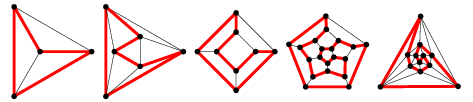
\includegraphics[scale=0.5]{img/PlatonicHamiltonian.png}
\end{center}
\item Soit $n$ le nombre de sommets du graphe. Les sommets sont tous de degré $n-1$. D'après un exercice de la feuille $1$, il existe un cycle de longueur $n$, que l'on peut construire étape par étape, en partant de n'importe quel sommet. A l'étape $k$, avec $1\leq k\leq n-1$, on dispose donc d'un chemin élémentaire ayant $k$ sommets distincts. Parmi les $n-1$ sommets adjacents du dernier sommet, il y a les $k-1$ prédécesseurs du dernier sommet, on choisit un successeur parmi les $n-k$ voisins restants. Ceci construit un chemin hamiltonien passant par tous les sommets. Comme le graphe est complet, on peut relier le premier au dernier point, ce qui donne un cycle hamiltonien.
\item Par récurrence sur le nombre de sommets.
\end{enumerate}
\end{Soln}
\begin{Soln}{100}
Sur le côté $[AB]$ du triangle, les couleurs des sommets de la triangulation changent un nombre impair de fois (autrement, les couleurs de $A$ et $B$ seraient les mêmes).

On en déduit que le sommet du graphe extérieur au triangle est de degré impair.

Or, on sait que dans un graphe, le nombre de sommets de degré impair est pair. Il reste donc un nombre impair de sommets impairs à l'intérieur du triangle.

Dans le triangle, le degré d'un sommet peut être $0$, $1$ ou $2$ mais pas $3$, et le cas du degré $1$ correspond au cas d'un triangle dont les sommets sont de trois couleurs distinctes. C'est aussi le seul cas où le degré est impair.

On en déduit qu'il existe à l'intérieur du triangle un nombre impair de sommets du graphe de degré $1$, et donc qu'il existe dans le triangle $ABC$ un nombre impair de triangles tricolores.
\end{Soln}
\begin{Soln}{101}
Construisons un triangle $AIB$ isocèle rectangle en $I$ et le cercle de centre $I$ et de rayon $IA$. Ce cercle intersecte la médiatrice de $[AB]$ en un point $O$ qui vérifie $\widehat{AOB}=\pm \pi/4$, par le théorème de l'angle au centre. C'est donc le centre d'un octogone appuyé sur $[AB]$. En traçant le cercle de centre $O$ et de rayon $OA$, on peut terminer la construction de cet octogone.
\end{Soln}
\begin{Soln}{102}
Commençons par rappeler deux points:
\begin{enumerate}
\item dans un trapèze, deux angles non adjacents à une même base sont supplémentaires, puisque les deux bases sont parallèles.
\item un quadrilatère non croisé est inscriptible ssi les angles opposés sont supplémentaires.
\end{enumerate}

Un trapèze est isocèle ssi les angles adjacents à une même base sont égaux, donc (par le premier point ci-dessus) ssi les angles opposés sont supplémentaires, donc (par le deuxième point) ssi il est inscriptible.

\begin{center}
\definecolor{qqwuqq}{rgb}{0.,0.39215686274509803,0.}
\definecolor{uuuuuu}{rgb}{0.26666666666666666,0.26666666666666666,0.26666666666666666}
\definecolor{qqqqff}{rgb}{0.,0.,1.}
\begin{tikzpicture}[line cap=round,line join=round,>=triangle 45,x=1.0cm,y=1.0cm]
\clip(-1.76,-0.56) rectangle (4.66,5.42);
\draw [shift={(1.94,4.96)},color=qqwuqq,fill=qqwuqq,fill opacity=0.1] (0,0) -- (-149.61179814845522:0.6) arc (-149.61179814845522:-47.299703593483734:0.6) -- cycle;
\draw [shift={(-0.36,0.18)},color=qqwuqq,fill=qqwuqq,fill opacity=0.1] (0,0) -- (30.388201851544782:0.6) arc (30.388201851544782:108.07610729657328:0.6) -- cycle;
\draw [shift={(-1.3,3.06)},color=qqwuqq,fill=qqwuqq,fill opacity=0.1] (0,0) -- (-71.92389270342673:0.6) arc (-71.92389270342673:30.388201851544792:0.6) -- cycle;
\draw(1.3116327852336915,2.319005145180441) circle (2.71471898725753cm);
\draw (-1.3,3.06)-- (1.94,4.96);
\draw (-1.3,3.06)-- (-0.36,0.18);
\draw (-0.36,0.18)-- (3.9945107601576444,2.7335711247838033);
\draw (3.9945107601576444,2.7335711247838033)-- (1.94,4.96);
\draw [shift={(-0.36,0.18)},color=qqwuqq] (30.388201851544782:0.6) arc (30.388201851544782:108.07610729657328:0.6);
\draw [shift={(-0.36,0.18)},color=qqwuqq] (30.388201851544782:0.5) arc (30.388201851544782:108.07610729657328:0.5);
\begin{scriptsize}
\draw [fill=qqqqff] (-0.36,0.18) circle (2.5pt);
\draw[color=qqqqff] (-0.74,-0.01) node {$A$};
\draw [fill=qqqqff] (-1.3,3.06) circle (2.5pt);
\draw[color=qqqqff] (-1.64,3.33) node {$B$};
\draw [fill=qqqqff] (1.94,4.96) circle (2.5pt);
\draw[color=qqqqff] (2.08,5.27) node {$C$};
\draw [fill=uuuuuu] (3.9945107601576444,2.7335711247838033) circle (1.5pt);
\draw[color=uuuuuu] (4.28,2.81) node {$D$};
\end{scriptsize}
\end{tikzpicture}
\end{center}

\end{Soln}
\begin{Soln}{104}
Traçons une figure. \emph{On marque dès à présent quelques égalités d'angles obtenues par le théorème de l'angle inscrit:}

\begin{center}
\begin{tikzpicture}[line cap=round,line join=round,>=triangle 45,x=1.0cm,y=1.0cm]
\clip(-6.84,-1.3) rectangle (3.34,5.62);
\draw [shift={(-4.54135770173771,2.073391502619976)},color=qqwuqq,fill=qqwuqq,fill opacity=0.1] (0,0) -- (-57.19135026317228:0.6) arc (-57.19135026317228:19.883254180671244:0.6) -- cycle;
\draw [shift={(-0.9357905924919852,-0.14942814068146326)},color=qqwuqq,fill=qqwuqq,pattern=north east lines,pattern color=qqwuqq] (0,0) -- (76.27770286686645:0.5) arc (76.27770286686645:179.20309842302296:0.5) -- cycle;
\draw [shift={(-1.7679241049654213,3.0764437353898777)},color=qqwuqq,fill=qqwuqq,fill opacity=0.1] (0,0) -- (-57.191350263172325:0.6) arc (-57.191350263172325:19.88325418067124:0.6) -- cycle;
\draw [shift={(-0.9357905924919852,-0.14942814068146326)},color=qqwuqq,fill=qqwuqq,fill opacity=0.1] (0,0) -- (-0.7969015769770713:0.6) arc (-0.7969015769770713:76.27770286686646:0.6) -- cycle;
\draw(-2.,2.16) circle (2.5428330656966063cm);
\draw(-0.28,1.74) circle (2.cm);
\draw [domain=-6.84:3.34] plot(\x,{(--9.256772261245349--0.9009661428453959*\x)/2.4911661511599217});
\draw [domain=-6.84:3.34] plot(\x,{(-0.5906140983383479-0.05057185931853675*\x)/3.6357905924919853});
\draw [color=ffqqqq,domain=-6.84:3.34] plot(\x,{(-7.025760591657469-2.192326777340297*\x)/1.4133266677517589});
\draw [color=ffqqqq,domain=-6.84:3.34] plot(\x,{(-0.6985138943712147--3.2433807595236943*\x)/-2.090909333629991});
\draw [dash pattern=on 3pt off 3pt] (-0.9357905924919852,-0.14942814068146326)-- (0.008833848840078207,3.719033857154604);
\begin{scriptsize}
\draw [fill=uuuuuu] (0.008833848840078207,3.719033857154604) circle (1.5pt);
\draw[color=uuuuuu] (0.12,4.12) node {$A$};
\draw [fill=uuuuuu] (-0.9357905924919852,-0.14942814068146326) circle (1.5pt);
\draw[color=uuuuuu] (-0.92,-0.4) node {$B$};
\draw [fill=uuuuuu] (-4.54135770173771,2.073391502619976) circle (1.5pt);
\draw[color=uuuuuu] (-4.96,2.32) node {$C$};
\draw [fill=uuuuuu] (-3.1280310339859514,-0.11893527472032112) circle (1.5pt);
\draw[color=uuuuuu] (-3.24,-0.3) node {$D$};
\draw [fill=uuuuuu] (-1.7679241049654213,3.0764437353898777) circle (1.5pt);
\draw[color=uuuuuu] (-1.72,3.56) node {$E$};
\draw [fill=uuuuuu] (0.32298522866456997,-0.1669370241338166) circle (1.5pt);
\draw[color=uuuuuu] (0.28,-0.4) node {$F$};
\end{scriptsize}
\end{tikzpicture}
\end{center}

\emph{Les égalités d'angles repérées sur la figure permettent de voir la solution, au moins dans la configuration particulière dessinée. On voit en effet que les angles $\widehat{ECD}$ et $\widehat{AEF}$ sont égaux. Attention toutefois, les angles géométriques sont trompeurs et les égalités que l'on voit sur une figure peuvent dépendre de la façon de tracer la figure. Sur la figure ci-dessous par exemple, les angles en question ne sont pas égaux mais supplémentaires.}

\begin{center}
\begin{tikzpicture}[line cap=round,line join=round,>=triangle 45,x=1.0cm,y=1.0cm]
\clip(-6.82,-1.14) rectangle (3.36,5.7);
\draw [shift={(-3.11,4.35)},color=qqwuqq,fill=qqwuqq,fill opacity=0.1] (0,0) -- (-111.67:0.6) arc (-111.67:-15.58:0.6) -- cycle;
\draw [shift={(-0.76,1.49)},color=qqwuqq,fill=qqwuqq,pattern=north east lines,pattern color=qqwuqq] (0,0) -- (96.63:0.5) arc (96.63:180.54:0.5) -- cycle;
\draw [shift={(-0.76,1.49)},color=qqwuqq,fill=qqwuqq,fill opacity=0.1] (0,0) -- (0.54:0.6) arc (0.54:96.63:0.6) -- cycle;
\draw [shift={(1.53,3.06)},color=qqwuqq,fill=qqwuqq,pattern=north east lines,pattern color=qqwuqq] (0,0) -- (164.42:0.6) arc (164.42:248.33:0.6) -- cycle;
\draw(-2.52,2.44) circle (2cm);
\draw(0.06,2.74) circle (1.5cm);
\draw [domain=-6.82:3.36] plot(\x,{(--15.16-1.21*\x)/4.35});
\draw [domain=-6.82:3.36] plot(\x,{(--5.5--0.03*\x)/3.68});
\draw [color=ffqqqq,domain=-6.82:3.36] plot(\x,{(-14.02-2.9*\x)/-1.15});
\draw [color=ffqqqq,domain=-6.82:3.36] plot(\x,{(-0.48--1.56*\x)/0.62});
\draw [dash pattern=on 2pt off 2pt] (-0.76,1.49)-- (-1.03,3.77);
\begin{scriptsize}
\draw [fill=uuuuuu] (-1.03,3.77) circle (1.5pt);
\draw[color=uuuuuu] (-0.88,4.16) node {$A$};
\draw [fill=uuuuuu] (-0.76,1.49) circle (1.5pt);
\draw[color=uuuuuu] (-0.74,1.2) node {$B$};
\draw [fill=uuuuuu] (-3.11,4.35) circle (1.5pt);
\draw[color=uuuuuu] (-3.38,4.7) node {$C$};
\draw [fill=uuuuuu] (-4.26,1.45) circle (1.5pt);
\draw[color=uuuuuu] (-4.56,1.28) node {$D$};
\draw [fill=uuuuuu] (1.53,3.06) circle (1.5pt);
\draw[color=uuuuuu] (1.56,3.52) node {$E$};
\draw [fill=uuuuuu] (0.91,1.5) circle (1.5pt);
\draw[color=uuuuuu] (1,1.24) node {$F$};
\end{scriptsize}
\end{tikzpicture}
\end{center}

\emph{Il ne reste plus qu'à rédiger rigoureusement la solution  avec des angles orientés de droites, en s'appuyant sur l'intuition donnée par la figure.}

Pour montrer que $(CD)$ et $(EF)$ sont parallèles, il suffit par exemple de montrer qu'elles forment le même angle avec la droite $(CA)$. Or on a la suite d'égalités d'angles de droites :

\begin{align*}
(CD,CA) &= (BD,BA) \text{ car $CDAB$ est inscriptible}\\
&= (BF,BA) \text{ car $(BD)=(BF)$}\\
&=(EF,EA) \text{ car $BFAE$ est inscriptible}\\
&=(EF,CA)  \text{ car $(EA)=(CA)$.}
\end{align*}

\end{Soln}
\begin{Soln}{105}

Pour montrer le résultat, il suffit de montrer que $IBC$ et $JBC$ sont isocèles en $I$ et $J$.

On rédige avec des angles de droites, ce qui a l'avantage de démontrer simultanément le résultat pour la bissectrice intérieure et extérieure.

En effet, les angles de droites ne voient pas la différence entre une bissectrice intérieure et extérieure : étant données deux droites $\mathcal D$ et $\mathcal D'$, une droite $\Delta$ est une bissectrice si
\[(\mathcal D,\Delta) = (\Delta,\mathcal D').\]
 Deux droites ont deux bissectrices. On ne peut distinguer les deux bissectrices que si on fixe des vecteurs directeurs des droites.

On prend donc une bissectrice (intérieure sur la figure mais ça ne changera rien), et on marque les angles égaux sur la figure :

\begin{tikzpicture}[line cap=round,line join=round,>=triangle 45,x=0.6235592739369882cm,y=0.6235592739369843cm]
\clip(1.98,-10.03) rectangle (18.02,6.01);
\draw [shift={(15.92,-5.44)},color=qqwuqq,fill=qqwuqq,fill opacity=0.1] (0,0) -- (180.39:1.24) arc (180.39:214.67:1.24) -- cycle;
\draw [shift={(8.29,2.24)},color=qqwuqq,fill=qqwuqq,fill opacity=0.1] (0,0) -- (-113.74:1.24) arc (-113.74:-79.46:1.24) -- cycle;
\draw [shift={(8.29,2.24)},color=qqwuqq,fill=qqwuqq,pattern=north east lines,pattern color=qqwuqq] (0,0) -- (-79.46:1.24) arc (-79.46:-45.19:1.24) -- cycle;
\draw [shift={(4.88,-5.51)},color=qqwuqq,fill=qqwuqq,pattern=north east lines,pattern color=qqwuqq] (0,0) -- (-33.88:1.24) arc (-33.88:0.39:1.24) -- cycle;
\draw(10.38,-3.31) ellipse (3.7cm and 3.7cm);
\draw (4.88,-5.51)-- (8.29,2.24);
\draw (15.92,-5.44)-- (4.88,-5.51);
\draw (8.29,2.24)-- (15.92,-5.44);
\draw [domain=1.98:18.02] plot(\x,{(-8.56--0.98*\x)/-0.18});
\draw [dash pattern=on 7pt off 7pt] (10.42,-9.24)-- (15.92,-5.44);
\draw [dash pattern=on 7pt off 7pt] (10.42,-9.24)-- (4.88,-5.51);
\begin{scriptsize}
\draw [fill=qqqqff] (8.29,2.24) circle (1.5pt);
\draw[color=qqqqff] (8.62,2.79) node {$A$};
\draw [fill=qqqqff] (4.88,-5.51) circle (1.5pt);
\draw[color=qqqqff] (4.21,-5) node {$B$};
\draw [fill=qqqqff] (15.92,-5.44) circle (1.5pt);
\draw[color=qqqqff] (16.7,-5.24) node {$C$};
\draw [fill=uuuuuu] (10.42,-9.24) circle (1.5pt);
\draw[color=uuuuuu] (10.06,-9.61) node {$I$};
\end{scriptsize}
\end{tikzpicture}

Pour montrer que $BCI$ est isocèle en $I$, il suffit de montrer que $(BC,BI) = (CI,CB)$. Or, on a
\begin{align*}
(BC,BI) &= (AC,AI) \text{ car $ABIC$ est inscriptible}\\
&= (AI,AB) \text{ car $(AI)$ est une bissectrice de $(AC)$ et $(AB)$}\\
&= (CI,CB) \text{ car $ABIC$ est inscriptible.}
\end{align*}

On vérifie que la même preuve marche pour l'autre bissectrice en remplaçant $I$ par $J$, tracée sur la figure ci-dessous :

\begin{tikzpicture}[line cap=round,line join=round,>=triangle 45,x=0.6235592739369882cm,y=0.6235592739369843cm]
\clip(1.98,-10.03) rectangle (18.02,6.01);
\draw [shift={(4.88,-5.51)},color=qqwuqq,fill=qqwuqq,fill opacity=0.1] (0,0) -- (0.39:1.24) arc (0.39:56.12:1.24) -- cycle;
\draw [shift={(8.29,2.24)},color=qqwuqq,fill=qqwuqq,fill opacity=0.1] (0,0) -- (-45.19:1.24) arc (-45.19:10.54:1.24) -- cycle;
\draw [shift={(8.29,2.24)},color=qqwuqq,fill=qqwuqq,pattern=north east lines,pattern color=qqwuqq] (0,0) -- (-169.46:1.24) arc (-169.46:-113.74:1.24) -- cycle;
\draw [shift={(15.92,-5.44)},color=qqwuqq,fill=qqwuqq,pattern=north east lines,pattern color=qqwuqq] (0,0) -- (124.67:1.24) arc (124.67:180.39:1.24) -- cycle;
\draw(10.38,-3.31) ellipse (3.7cm and 3.7cm);
\draw (4.88,-5.51)-- (8.29,2.24);
\draw (15.92,-5.44)-- (4.88,-5.51);
\draw (8.29,2.24)-- (15.92,-5.44);
\draw [domain=1.98:18.02] plot(\x,{(--0.69--0.18*\x)/0.98});
\draw [domain=1.98:18.02] plot(\x,{(-8.56--0.98*\x)/-0.18});
\draw [dash pattern=on 7pt off 7pt] (4.88,-5.51)-- (10.34,2.62);
\draw [dash pattern=on 7pt off 7pt] (10.34,2.62)-- (15.92,-5.44);
\begin{scriptsize}
\draw [fill=qqqqff] (8.29,2.24) circle (1.5pt);
\draw[color=qqqqff] (8.62,2.79) node {$A$};
\draw [fill=qqqqff] (4.88,-5.51) circle (1.5pt);
\draw[color=qqqqff] (4.21,-5) node {$B$};
\draw [fill=qqqqff] (15.92,-5.44) circle (1.5pt);
\draw[color=qqqqff] (16.7,-5.24) node {$C$};
\draw [fill=uuuuuu] (10.34,2.62) circle (1.5pt);
\draw[color=uuuuuu] (10.81,3.5) node {$J$};
\end{scriptsize}
\end{tikzpicture}



\emph{Si on rédige avec des angles orientés de vecteurs et non de droites, on doit faire attention aux éventuels facteurs $\pi$ qui apparaissent suivant si on considère la bissectrice intérieure ou extérieure d'un couple de vecteurs.}

\end{Soln}
\begin{Soln}{106}


\begin{tikzpicture}[line cap=round,line join=round,>=triangle 45,x=1.0cm,y=1.0cm]
\clip(-2,-3) rectangle (14.8,5);
\fill[fill opacity=0] (1.14,-0.9) -- (4.52,4.14) -- (8.8,-2.26) -- cycle;
\draw  (1.14,-0.9)-- (4.52,4.14);
\draw  (4.52,4.14)-- (8.8,-2.26);
\draw  (8.8,-2.26)-- (1.14,-0.9);
\draw(5.25,0) circle (4.21cm);
\draw(3.52,-1.53) circle (2.46cm);
\draw [dashed] (3.24,2.31) circle (2.24cm);
\draw(7.88,0.79) circle (3.18cm);
\begin{scriptsize}
\draw (1.3,-0.64) node [right] {$A$};
\draw (4.66,4.4) node {$C$};
\draw (8.96,-2) node [above] {$B$};
\draw (2.18,0.68) node [above] {$Q$};
\draw (5.58,3.06) node {$P$};
\draw (6.14,-1.5) node {$R$};
\draw (4.86,0.88) node {$T$};
\end{scriptsize}
\end{tikzpicture}


Il suffit de montrer que $T, P, C, Q$ sont cocycliques. Voici plusieurs rédactions possibles.

\underline{Rédaction avec des angles non orientés:}\\
Il suffit par le cours de montrer que les angles $\widehat{TPC}$ et $\widehat{TQC}$ sont supplémentaires. Or par construction, les couples suivants d'angles sont supplémentaire: \\
$\widehat{TQC}$ et $\widehat{TQA}$ car $Q\in[AC]$,\\
$\widehat{TQA}$ et $\widehat{TRA}$ car $TQAR$ est inscriptible dans cet ordre,\\
$\widehat{TRA}$ et $\widehat{TRB}$ car $R\in[AB]$,\\
$\widehat{TRB}$ et $\widehat{TPB}$ car $TRBP$ est inscriptible dans cet ordre,\\
$\widehat{TPB}$ et $\widehat{TPC}$ car $P \in[BC]$.\\
On en déduit immédiatement que $\widehat{TQC}=\widehat{TRA}=\widehat{TPB}$ et $\widehat{TQA}=\widehat{TRB}=\widehat{TPC}$ sont supplémentaires.

\emph{Une rédaction avec des angles non orientés est difficile à suivre sans figure : il faut bien justifier la cocyclicité dans un ordre précis pour que les angles inscrits soient supplémentaires et non égaux, et cela peut dépendre de la figure. Il faut donc parfois distinguer artificiellement plusieurs cas. La rédaction qui suit élimine ce problème.}


\underline{Rédaction avec des angles de droites}:\\
Par le cours,  il suffit de montrer l'égalité d'angles de droites $(QT,QC)=(PT,PC)$. Or on a :
\begin{align*}
(QT,QC)&=(QT,QA) \text{ car $(QC)=(QA)$}\\
&=(RT,RA) \text{ car $AQTR$ est inscriptible} \\
&= (RT,RB) \text{ car $(RA)=(RB)$} \\
&=(PT,PB) \text{ car $PTRB$ est inscriptible} \\
&=(PT,PC) \text{ car $(PB)=(PC)$.}
\end{align*}
\emph{La rédaction avec des angles de droites est sans doute la plus efficace pour ce type d'exercice : elle conserve les avantages des angles orientés de vecteurs (Chasles, calculs faciles à suivre même sans figure), et simplifie la rédaction lorsqu'il y a des angles supplémentaires.}
\end{Soln}
\begin{Soln}{107}
Traçons une figure :
\begin{center}

\begin{tikzpicture}[line cap=round,line join=round,>=triangle 45,x=0.6049844578223686cm,y=0.6099433468209144cm]
\clip(-3.752802476086023,-3.2338432364622567) rectangle (6.164807674754709,6.603135937542343);
\draw [shift={(-1.22,5.12)},color=qqwuqq,fill=qqwuqq,fill opacity=0.1] (0,0) -- (-28.790811275069014:0.8063097683610351) arc (-28.790811275069014:3.373433258452694:0.8063097683610351) -- cycle;
\draw [shift={(5.3029984172619935,1.53531343775139)},color=qqwuqq,fill=qqwuqq,fill opacity=0.1] (0,0) -- (119.04494419140927:0.8063097683610351) arc (119.04494419140927:151.20918872493098:0.8063097683610351) -- cycle;
\draw [shift={(-0.33735270489567304,-2.0802136358470724)},color=qqwuqq,fill=qqwuqq,fill opacity=0.1] (0,0) -- (64.82456240918293:0.8063097683610351) arc (64.82456240918293:96.98880694270463:0.8063097683610351) -- cycle;
\draw [shift={(3.1686365489609396,5.378691016947528)},color=ffqqqq,fill=ffqqqq,fill opacity=0.1] (0,0) -- (-176.62656674154732:0.6719248069675292) arc (-176.62656674154732:-162.60293692157978:0.6719248069675292) -- cycle;
\draw [shift={(-0.33735270489567304,-2.0802136358470724)},color=ffqqqq,fill=ffqqqq,fill opacity=0.1] (0,0) -- (96.98880694270463:0.8063097683610351) arc (96.98880694270463:111.01243676267217:0.8063097683610351) -- cycle;
\draw [shift={(0.07379462482048285,4.409000562436103)},color=qqwuqq,fill=qqwuqq,pattern=north east lines,pattern color=qqwuqq] (0,0) -- (-162.60293692157978:0.40315488418051754) arc (-162.60293692157978:-28.790811275069014:0.40315488418051754) -- cycle;
\draw [shift={(0.07379462482048285,4.409000562436103)},color=qqwuqq,fill=qqwuqq,pattern=north east lines,pattern color=qqwuqq] (0,0) -- (17.397063078420217:0.40315488418051754) arc (17.397063078420217:151.20918872493095:0.40315488418051754) -- cycle;
\draw [line width=1.2pt] (1.18,1.76) ellipse (2.4980510820928545cm and 2.518526910634607cm);
\draw [line width=1.2pt] (-1.22,5.12)-- (5.3029984172619935,1.53531343775139);
\draw [line width=1.2pt] (3.1686365489609396,5.378691016947528)-- (-2.5180150920511677,3.5969225293848943);
\draw [line width=1.2pt] (3.1686365489609396,5.378691016947528)-- (-0.33735270489567304,-2.0802136358470724);
\draw [dash pattern=on 2pt off 2pt] (-2.5180150920511677,3.5969225293848943)-- (-1.22,5.12);
\draw [dash pattern=on 2pt off 2pt] (-0.33735270489567304,-2.0802136358470724)-- (5.3029984172619935,1.53531343775139);
\draw [dash pattern=on 2pt off 2pt] (-0.33735270489567304,-2.0802136358470724)-- (-2.5180150920511677,3.5969225293848943);
\draw [dash pattern=on 2pt off 2pt] (-0.33735270489567304,-2.0802136358470724)-- (-1.22,5.12);
\draw [dash pattern=on 2pt off 2pt] (-1.22,5.12)-- (3.1686365489609396,5.378691016947528);
\draw [dash pattern=on 2pt off 2pt] (3.1686365489609396,5.378691016947528)-- (5.3029984172619935,1.53531343775139);
\draw [dash pattern=on 2pt off 2pt] (5.3029984172619935,1.53531343775139)-- (-2.5180150920511677,3.5969225293848943);
\begin{scriptsize}
\draw [fill=qqqqff] (-1.22,5.12) circle (2.5pt);
\draw[color=qqqqff] (-1.0382262559372046,5.608687223230403) node {$B$};
\draw [fill=xdxdff] (5.3029984172619935,1.53531343775139) circle (2.5pt);
\draw[color=xdxdff] (5.49288286778718,2.0071702578844564) node {$C$};
\draw [fill=uuuuuu] (3.1686365489609396,5.378691016947528) circle (1.5pt);
\draw[color=uuuuuu] (3.3696004777697866,5.743072184623909) node {$A$};
\draw [fill=xdxdff] (-2.5180150920511677,3.5969225293848943) circle (2.5pt);
\draw[color=xdxdff] (-3.0271236845610914,4.103575655623142) node {$D$};
\draw [fill=xdxdff] (-0.33735270489567304,-2.0802136358470724) circle (2.5pt);
\draw[color=xdxdff] (-0.7425793408714919,-2.185640537592914) node {$E$};
\draw [fill=uuuuuu] (0.07379462482048285,4.409000562436103) circle (1.5pt);
\draw[color=uuuuuu] (0.06373042748954315,3.8348057328361307) node {$F$};
\draw [fill=uuuuuu] (2.171091873144122,3.256439610832737) circle (1.5pt);
\draw[color=uuuuuu] (1.4882110182607051,3.270388894983408) node {$G$};
\end{scriptsize}
\end{tikzpicture}
\begin{tikzpicture}[line cap=round,line join=round,>=triangle 45,x=0.6049844578223686cm,y=0.6099433468209144cm]
\clip(-3.752802476086023,-3.2338432364622567) rectangle (6.164807674754709,6.603135937542343);
\draw [line width=1.2pt] (1.18,1.76) ellipse (2.4980510820928545cm and 2.518526910634607cm);
\draw [line width=1.2pt] (-1.22,5.12)-- (5.3029984172619935,1.53531343775139);
\draw [line width=1.2pt] (3.1686365489609396,5.378691016947528)-- (-2.5180150920511677,3.5969225293848943);
\draw [line width=1.2pt] (3.1686365489609396,5.378691016947528)-- (-0.33735270489567304,-2.0802136358470724);
\draw [dash pattern=on 2pt off 2pt,color=ffqqqq] (-0.33678647441899345,1.1773824411032867) ellipse (1.9707950261897778cm and 1.9869490837815031cm);
\begin{scriptsize}
\draw [fill=qqqqff] (-1.22,5.12) circle (2.5pt);
\draw[color=qqqqff] (-1.0382262559372046,5.608687223230403) node {$B$};
\draw [fill=xdxdff] (5.3029984172619935,1.53531343775139) circle (2.5pt);
\draw[color=xdxdff] (5.49288286778718,2.0071702578844564) node {$C$};
\draw [fill=uuuuuu] (3.1686365489609396,5.378691016947528) circle (1.5pt);
\draw[color=uuuuuu] (3.3696004777697866,5.743072184623909) node {$A$};
\draw [fill=xdxdff] (-2.5180150920511677,3.5969225293848943) circle (2.5pt);
\draw[color=xdxdff] (-3.0271236845610914,4.103575655623142) node {$D$};
\draw [fill=xdxdff] (-0.33735270489567304,-2.0802136358470724) circle (2.5pt);
\draw[color=xdxdff] (-0.7425793408714919,-2.185640537592914) node {$E$};
\draw [fill=uuuuuu] (0.07379462482048285,4.409000562436103) circle (1.5pt);
\draw[color=uuuuuu] (0.06373042748954315,3.8348057328361307) node {$F$};
\draw [fill=uuuuuu] (2.171091873144122,3.256439610832737) circle (1.5pt);
\draw[color=uuuuuu] (1.4882110182607051,3.270388894983408) node {$G$};
\end{scriptsize}
\end{tikzpicture}

\end{center}

\emph{[Sur la figure, on voit que les angles $\widehat{GFD}$ et $\widehat{GED}$ sont supplémentaires, car $\widehat{GFD}=\widehat{BFA}$ et $\widehat{GED}=\widehat{GEB}+\widehat{BED} = \widehat{FBA}+\widehat{BAF}$. Il ne reste plus qu'à rédiger cette preuve un peu plus rigoureusement avec des angles de droites.]}

Montrons que $(FD,FG)=(ED,EG)$, ce qui prouve que $EDFG$ est inscriptible.

Tout d'abord, comme $(FD)=(FA)$ et $(FG)=(FB)$, on a
\[(FD,FG)=(FA,FB).\]

Ensuite, la somme des angles du triangle $ABF$ vaut $\pi$, donc en termes d'angles de droites on a la relation
$(FA,FB)+(AB,AF)+(BF,BA)=0$, c'est-à-dire:
\[
(FA,FB) = (AF,AB)+(BA,BF).
\]
Calculons chacun de ces deux angles. D'une part, on a :
\begin{align*}
(AF,AB) &= (AD,AB) \text{ car $(AD)=(AF)$}\\
&=(ED,EB) \text{ car $ABDE$ est inscriptible}.
\end{align*}
Et d'autre part :
\begin{align*}
(BA,BF) &= (BA,BC) \text{ car $(BF)=(BC)$} \\
&= (CB,CA) \text{ car $ABC$ est isocèle en $A$}\\
&= (EB,EA) \text{ car $ABCE$ est inscriptible.}
\end{align*}

Finalement, on obtient donc:
\begin{align*}
(FD,FG)&=(FA,FB) \\
&= (AF,AB)+(BA,BF) \\
&= (ED,EB) + (EB,EA)\\
&= (ED,EA)\\
&= (ED,EG) \text{ car $(EG)=(EA)$,}
\end{align*}
ce qu'il fallait démontrer.

% solution rédigée différemment sur le pdf

\end{Soln}
\begin{Soln}{108}
 Traçons une figure. \emph{[Comme d'habitude, le fait de marquer toutes les égalités d'angles disponibles donne le résultat. Sur la figure, on ne marque que celles utilisées dans la rédaction proposée.]}
\begin{center}
\begin{tikzpicture}[line cap=round,line join=round,>=triangle 45,x=1.0cm,y=1.0cm]
\clip(-5.79,-2.53) rectangle (11.17,8.14);
\draw [shift={(9.02,1.97)},color=ffqqqq,fill=ffqqqq,fill opacity=0.1] (0,0) -- (-179.31:1.4) arc (-179.31:-166.83:1.4) -- cycle;
\draw [shift={(1.97,5.91)},color=ffqqqq,fill=ffqqqq,fill opacity=0.1] (0,0) -- (-105.64:1.4) arc (-105.64:-93.16:1.4) -- cycle;
\draw [shift={(1.97,5.91)},color=qqwuqq,fill=qqwuqq,fill opacity=0.1] (0,0) -- (-146.73:0.84) arc (-146.73:-93.16:0.84) -- cycle;
\draw [shift={(2.85,1.9)},color=qqwuqq,fill=qqwuqq,fill opacity=0.1] (0,0) -- (-179.31:0.84) arc (-179.31:-125.74:0.84) -- cycle;
\draw(-0.73,3.22) circle (3.81cm);
\draw(4.92,2.91) circle (4.21cm);
\draw [domain=-5.79:11.17] plot(\x,{(--9.53--0.06*\x)/5.12});
\draw (-4.27,1.81)-- (1.97,5.91);
\draw (1.97,5.91)-- (0.84,1.87);
\draw (2.85,1.9)-- (1.66,0.25);
\draw (9.02,1.97)-- (1.66,0.25);
\draw [dash pattern=on 4pt off 4pt] (1.97,5.91)-- (1.66,0.25);
\begin{scriptsize}
\draw [fill=qqqqff] (1.97,5.91) circle (1.5pt);
\draw[color=qqqqff] (1.98,6.44) node {$P$};
\draw [fill=qqqqff] (1.66,0.25) circle (1.5pt);
\draw[color=qqqqff] (1.7,-0.16) node {$Q$};
\draw [fill=qqqqff] (-4.27,1.81) circle (1.5pt);
\draw[color=qqqqff] (-4.78,2.19) node {$A$};
\draw [fill=qqqqff] (0.84,1.87) circle (1.5pt);
\draw[color=qqqqff] (0.44,1.52) node {$C$};
\draw [fill=uuuuuu] (2.85,1.9) circle (1.5pt);
\draw[color=uuuuuu] (3.29,1.63) node {$B$};
\draw [fill=uuuuuu] (9.02,1.97) circle (1.5pt);
\draw[color=uuuuuu] (9.24,2.33) node {$D$};
\end{scriptsize}
\end{tikzpicture}
\end{center}

Montrons que $(PA,PC)=(DQ,BQ)$. On a:
\begin{align*}
(PA,PC)&= (PA,PQ)+(PQ,PC) \\
&= (BA,BQ)+(DQ,DC) \text{ par cocyclicité dans chaque cercle}\\
&= (BA,BQ)+(DQ,BA) \text{ car $(DC)=(BA)$}\\
&= (DQ,BQ).
\end{align*}

\emph{[Voici une autre configuration possible pour la figure, la preuve reste inchangée :]}
\begin{center}
\begin{tikzpicture}[line cap=round,line join=round,>=triangle 45,x=1.0cm,y=1.0cm]
\clip(-5.79,-2.53) rectangle (11.17,8.14);
\draw [shift={(2.32,5.21)},color=qqwuqq,fill=qqwuqq,fill opacity=0.1] (0,0) -- (165.17:0.84) arc (165.17:271.19:0.84) -- cycle;
\draw [shift={(0.36,6.67)},color=qqwuqq,fill=qqwuqq,fill opacity=0.1] (0,0) -- (-175.75:0.84) arc (-175.75:-69.74:0.84) -- cycle;
\draw(-0.78,3.12) circle (3.73cm);
\draw(6.1,3.26) circle (4.25cm);
\draw [domain=-5.79:11.17] plot(\x,{(--42.51--0.47*\x)/6.4});
\draw (-2.43,6.46)-- (2.32,5.21);
\draw (2.32,5.21)-- (3.96,6.94);
\draw (0.36,6.67)-- (2.4,1.16);
\draw (7.66,7.21)-- (2.4,1.16);
\draw [dash pattern=on 4pt off 4pt] (2.32,5.21)-- (2.4,1.16);
\begin{scriptsize}
\draw [fill=qqqqff] (2.32,5.21) circle (1.5pt);
\draw[color=qqqqff] (2.32,5.74) node {$P$};
\draw [fill=qqqqff] (2.4,1.16) circle (1.5pt);
\draw[color=qqqqff] (2.43,0.74) node {$Q$};
\draw [fill=qqqqff] (-2.43,6.46) circle (1.5pt);
\draw[color=qqqqff] (-2.94,6.86) node {$A$};
\draw [fill=qqqqff] (3.96,6.94) circle (1.5pt);
\draw[color=qqqqff] (3.66,7.39) node {$C$};
\draw [fill=uuuuuu] (0.36,6.67) circle (1.5pt);
\draw[color=uuuuuu] (0.78,7.02) node {$B$};
\draw [fill=uuuuuu] (7.66,7.21) circle (1.5pt);
\draw[color=uuuuuu] (7.87,7.58) node {$D$};
\end{scriptsize}
\end{tikzpicture}
\end{center}
\end{Soln}
\begin{Soln}{109}
Le point $A$ appartient au cercle de diamètre $[EH]$.
\end{Soln}
\begin{Soln}{110}
Traçons la figure, où on a placé $I$ le milieu de $[AB]$, de telle sorte que $\frac12(OA,OB)=(OA,OI)$.

\begin{center}

\definecolor{qqwuqq}{rgb}{0.,0.39215686274509803,0.}
\definecolor{uuuuuu}{rgb}{0.26666666666666666,0.26666666666666666,0.26666666666666666}
\definecolor{xdxdff}{rgb}{0.49019607843137253,0.49019607843137253,1.}
\definecolor{qqqqff}{rgb}{0.,0.,1.}
\begin{tikzpicture}[line cap=round,line join=round,>=triangle 45,x=1.0cm,y=1.0cm]
\clip(4,-4) rectangle (14,3.8);
\draw [shift={(11.74187889933037,2.2246542567951373)},color=qqwuqq,fill=qqwuqq,fill opacity=0.1] (0,0) -- (164.80233009357863:0.5881327557490914) arc (164.80233009357863:200.02131119208804:0.5881327557490914) -- cycle;
\draw [shift={(10.106627303264904,-3.7950390448372655)},color=qqwuqq,fill=qqwuqq,fill opacity=0.1] (0,0) -- (74.80233009357865:0.5881327557490914) arc (74.80233009357865:110.02131119208799:0.5881327557490914) -- cycle;
\draw[color=qqwuqq,fill=qqwuqq,fill opacity=0.1] (8.504281918639839,0.6022789927301224) -- (8.89502145618116,0.744661165049919) -- (8.752639283861363,1.1354007025912407) -- (8.361899746320042,0.993018530271444) -- cycle;
\draw [shift={(11.74187889933037,2.2246542567951373)},color=qqwuqq,fill=qqwuqq,pattern=north east lines,pattern color=qqwuqq] (0,0) -- (-159.978688807912:0.6861548817072733) arc (-159.978688807912:-105.19766990642137:0.6861548817072733) -- cycle;
\draw[color=qqwuqq,fill=qqwuqq,fill opacity=0.1] (11.63285790928615,1.8233258464847182) -- (12.034186319596568,1.7143048564404975) -- (12.14320730964079,2.1156332667509163) -- (11.74187889933037,2.2246542567951373) -- cycle;
\draw(10.106627303264904,-3.7950390448372655) circle (6.237848605741619cm);
\draw [domain=2.5705762947384336:17.960050070172993] plot(\x,{(--32.592662539015095-1.6352515960654657*\x)/6.019693301632403});
\draw (10.106627303264904,-3.7950390448372655)-- (11.74187889933037,2.2246542567951373);
\draw (10.106627303264904,-3.7950390448372655)-- (4.9819205933097095,-0.23861719625224892);
\draw (11.74187889933037,2.2246542567951373)-- (4.9819205933097095,-0.23861719625224892);
\draw [dash pattern=on 2pt off 2pt,domain=2.5705762947384336:17.960050070172993] plot(\x,{(-58.972167842212926--6.7599583060206605*\x)/-2.463271453047386});
\begin{scriptsize}
\draw [fill=qqqqff] (10.106627303264904,-3.7950390448372655) circle (1.5pt);
\draw[color=qqqqff] (10.412346371392987,-3.7282048803635246) node {$O$};
\draw [fill=qqqqff] (4.9819205933097095,-0.23861719625224892) circle (1.5pt);
\draw[color=qqqqff] (4.413392262752254,-0.042572944335882046) node {$B$};
\draw [fill=xdxdff] (11.74187889933037,2.2246542567951373) circle (1.5pt);
\draw[color=xdxdff] (11.80426055999917,2.682442157301577) node {$A$};
\draw [fill=uuuuuu] (8.361899746320042,0.993018530271444) circle (1.5pt);
\draw[color=uuuuuu] (8.491112702612622,1.2709235435037565) node {$I$};
\end{scriptsize}
\end{tikzpicture}
\end{center}


Les angles $(AO,\mathcal T)$ et $(AI,IO)$ sont droits.
On a d'une part :
\[ 0=(\mathcal T,\mathcal T) =  (\mathcal T,AI) +(AI,AO)+ \pi/2, \]
et d'autre part, dans le triangle $AIO$:
\[ 0=(AI,AO)+(IO,IA)+(OA,OI)=(AI,AO)+\pi/2+(OA,OI).\]
Finalement, on a donc:
\[ (\mathcal T,AB) = (\mathcal T, AI) = -(AI,AO)-\pi/2 = (OA,OI)=\frac{1}{2}(OA,OB),\]
ce qu'il fallait démontrer.$\qed$


\end{Soln}
\begin{Soln}{111}
Soit $\mathcal T$ la tangente commune  aux deux cercles.

\begin{center}
%\includegraphics{images/img007125-2}
\definecolor{qqwuqq}{rgb}{0.,0.39215686274509803,0.}
\definecolor{ffqqtt}{rgb}{1.,0.,0.2}
\definecolor{uuuuuu}{rgb}{0.26666666666666666,0.26666666666666666,0.26666666666666666}
\definecolor{xdxdff}{rgb}{0.49019607843137253,0.49019607843137253,1.}
\definecolor{qqqqff}{rgb}{0.,0.,1.}
\begin{tikzpicture}[line cap=round,line join=round,>=triangle 45,x=1.0cm,y=1.0cm]
\clip(-4.96,-1.2) rectangle (5.46,4.94);
\draw [shift={(-3.978047764643616,3.8381858014869974)},color=qqwuqq,fill=qqwuqq,fill opacity=0.1] (0,0) -- (-79.44755493537986:0.6) arc (-79.44755493537986:-21.02616489762143:0.6) -- cycle;
\draw [shift={(0.7,2.04)},color=qqwuqq,fill=qqwuqq,fill opacity=0.1] (0,0) -- (-147.57262576620485:0.6) arc (-147.57262576620485:-88.36342295838327:0.6) -- cycle;
\draw [shift={(4.319131555166006,0.6488489678538256)},color=qqwuqq,fill=qqwuqq,fill opacity=0.1] (0,0) -- (99.764632294557:0.6) arc (99.764632294557:158.9738351023786:0.6) -- cycle;
\draw(-2.,2.) circle (2.700296280040396cm);
\draw(2.8,2.1) circle (2.1008569680013913cm);
\draw [domain=-4.96:5.46] plot(\x,{(-10.801947500913874--1.7981858014869974*\x)/-4.678047764643616});
\draw [domain=-4.96:5.46] plot(\x,{(-6.195302419327594-2.4671338401188603*\x)/-3.8834784840249004});
\draw [color=ffqqtt,domain=-4.96:5.46] plot(\x,{(-13.917940734612198-4.265319641605858*\x)/0.7945692806187159});
\draw [color=ffqqtt,domain=-4.96:5.46] plot(\x,{(--14.73968797588983-3.326646488964469*\x)/0.5724971001338988});
\draw [dash pattern=on 5pt off 5pt,domain=-4.96:5.46] plot(\x,{(-1.5924--2.1*\x)/-0.06});
\begin{scriptsize}
\draw [fill=qqqqff] (0.7,2.04) circle (2.5pt);
\draw[color=qqqqff] (0.84,2.41) node {$T$};
\draw [fill=xdxdff] (-3.978047764643616,3.8381858014869974) circle (2.5pt);
\draw[color=xdxdff] (-4.6,3.87) node {$A$};
\draw [fill=xdxdff] (-3.1834784840249,-0.42713384011886024) circle (2.5pt);
\draw[color=xdxdff] (-3.84,-0.31) node {$B$};
\draw [fill=uuuuuu] (3.7466344550321073,3.9754954568182947) circle (1.5pt);
\draw[color=uuuuuu] (3.94,4.47) node {$B'$};
\draw [fill=uuuuuu] (4.319131555166006,0.6488489678538256) circle (1.5pt);
\draw[color=uuuuuu] (4.1,0.07) node {$A'$};
\end{scriptsize}
\end{tikzpicture}
\end{center}

Par le cas limite du théorème des angles inscrits, on a
\[ (AB,AT) = (BT,\mathcal T)=(B'T,\mathcal T)=(A'B',A'T)\]

Comme $(AT) = (A'T)$, on en déduit que
\[ (AB,AT) = (A'B',AT),\]
et donc que $(AB)//(A'B')$.

\underline{Autre preuve:} considérer une homothétie de centre $T$ qui envoie un cercle sur l'autre.

\end{Soln}
\begin{Soln}{112}

Le quadrilatère $ABA'B'$ est inscriptible dans un cercle de diamètre $[AB]$. En effet, les triangles $ABA'$ et $ABB'$ sont par définition rectangles en $A'$ et $B'$, et ont même hypoténuse $[AB]$.

De même, les quadrilatères $BCB'C'$ et $CAC'A'$ sont inscriptibles dans des cercles de diamètre $[BC]$ et $[CA]$.

\begin{center}
%\includegraphics{images/img007131-1}
\definecolor{qqwuqq}{rgb}{0.,0.39215686274509803,0.}
\definecolor{uuuuuu}{rgb}{0.26666666666666666,0.26666666666666666,0.26666666666666666}
\definecolor{xdxdff}{rgb}{0.49019607843137253,0.49019607843137253,1.}
\definecolor{qqqqff}{rgb}{0.,0.,1.}
\definecolor{qqwuqq}{rgb}{0,0.39,0}
\definecolor{uuuuuu}{rgb}{0.27,0.27,0.27}
\definecolor{xdxdff}{rgb}{0.49,0.49,1}
\definecolor{qqqqff}{rgb}{0,0,1}
\definecolor{ffqqqq}{rgb}{1.,0.,0.}

\begin{tikzpicture}[line cap=round,line join=round,>=triangle 45,x=1.0cm,y=1.0cm]
\clip(3.6292152550867987,-5.041701368203163) rectangle (16.68576243271663,3.6038501413084876);
\draw[color=qqwuqq,fill=qqwuqq,fill opacity=0.1] (8.268175288872698,-2.7715717860200795) -- (7.852814176986605,-2.750951021600202) -- (7.8321934125667285,-3.1663121334862936) -- (8.24755452445282,-3.186932897906171) -- cycle;
\draw[color=qqwuqq,fill=qqwuqq,fill opacity=0.1] (9.561507124932467,0.5418232874040516) -- (9.862989559441017,0.25536489448230715) -- (10.149447952362761,0.5568473289908564) -- (9.847965517854211,0.8433057219126009) -- cycle;
\draw[color=qqwuqq,fill=qqwuqq,fill opacity=0.1] (7.790587291843089,-0.4447648275939527) -- (7.964500456074173,-0.06700262660020309) -- (7.586738255080424,0.10691053763088143) -- (7.412825090849339,-0.27085166336286814) -- cycle;
\draw (6.1189772544246175,-3.0812588490395227)-- (8.510717127804256,2.113913826744122);
\draw (8.510717127804256,2.113913826744122)-- (14.411649110486806,-3.4929517780638872);
\draw (14.411649110486806,-3.4929517780638872)-- (6.1189772544246175,-3.0812588490395227);
\draw (8.510717127804256,2.113913826744122)-- (8.24755452445282,-3.186932897906171);
\draw (7.412825090849339,-0.27085166336286814)-- (14.411649110486806,-3.4929517780638872);
\draw (9.847965517854211,0.8433057219126009)-- (6.1189772544246175,-3.0812588490395227);
\draw [dash pattern=on 5pt off 5pt] (7.314847191114436,-0.4836725111477) circle (2.8596432799006175cm);
\draw [dash pattern=on 5pt off 5pt] (10.265313182455714,-3.287105313551705) circle (4.151442447515517cm);
\draw [dash pattern=on 5pt off 5pt] (11.461183119145531,-0.6895189756598837) circle (4.069949022242936cm);
\begin{scriptsize}
\draw [fill=qqqqff] (6.1189772544246175,-3.0812588490395227) circle (2.5pt);
\draw[color=qqqqff] (5.707284325400255,-3.179280974997705) node {$A$};
\draw [fill=qqqqff] (8.510717127804256,2.113913826744122) circle (2.5pt);
\draw[color=qqqqff] (8.510717127804257,2.525606755768486) node {$B$};
\draw [fill=qqqqff] (14.411649110486806,-3.4929517780638872) circle (2.5pt);
\draw[color=qqqqff] (14.7841331891279,-3.5909739040220696) node {$C$};
\draw [fill=uuuuuu] (9.847965517854211,0.8433057219126009) circle (1.5pt);
\draw[color=uuuuuu] (10.137884418710078,1.2709235435037565) node {$A'$};
\draw [fill=uuuuuu] (7.412825090849339,-0.27085166336286814) circle (1.5pt);
\draw[color=uuuuuu] (7.099198514006438,-0.022968519144245664) node {$C'$};
\draw [fill=uuuuuu] (8.24755452445282,-3.186932897906171) circle (1.5pt);
\draw[color=uuuuuu] (8.216650749929713,-3.5321606284471603) node {$B'$};
\end{scriptsize}
\end{tikzpicture}
\end{center}

Montrons que la hauteur $(BB')$ est une bissectrice des droites $(B'C')$ et $(B'A')$. Pour cela, on montre que $(B'C',B'B)=(B'B,B'A')$.

On a :
\begin{align*}
(B'C',B'B)
&= (CC',CB) \text{ (car $BCB'C'$ est inscriptible)}\\
&= (CC',CA') \text{ (mêmes droites)}\\
&= (AC'AA') \text{ (car $ACA'C'$ est inscriptible)}\\
&= (AB,AA') \text{ (mêmes droites)}\\
&= (B'B,B'A') \text{ (car $ABA'B'$ est inscriptible)}\\
\end{align*}

\end{Soln}
\begin{Soln}{115}

Si $ABC$ est rectangle, l'orthocentre coïncide avec un des sommets et la vérification de l'assertion est relativement facile. Dans la suite on suppose qu'on n'est pas dans ce cas.

Par définition, $H'$ est le symétrique de $H$ par rapport à $(AC)$ si $(AC)$ est la médiatrice de $[HH']$. C'est cela qu'on doit montrer.



D'autre part, par définition, on a $(AC) \bot (HH')$, donc $(AC)$ est la hauteur de $AHH'$ issue de $A$.

Donc si $AHH'$ est isocèle en $A$, alors cette hauteur de $AHH'$  est aussi la médiane issue de $A$ et c'est encore la médiatrice du côté opposé à $A$ c'est-à-dire $[HH']$.

Il suffit donc de montrer que $AHH'$ est isocèle en $A$. Pour cela, il suffit de montrer que les angles adjacents à la base sont égaux, autrement dit $\widehat{AHH'} = \widehat{AH'H}$ avec des angles géométriques non orientés, ou plus précisément avec des angles orientés $(H'A,H'H)=(HH',AH)$.

Suivant la méthodologie habituelle, on marque de façon systématique les angles égaux (ou complémentaires, supplémentaires etc) sur la figure. Ceci indique la marche à suivre pour la preuve.


\begin{center}
%\includegraphics{images/img007139-2}
\definecolor{qqwuqq}{rgb}{0.,0.39215686274509803,0.}
\definecolor{uuuuuu}{rgb}{0.26666666666666666,0.26666666666666666,0.26666666666666666}
\definecolor{qqqqff}{rgb}{0.,0.,1.}
\begin{tikzpicture}[line cap=round,line join=round,>=triangle 45,x=1.0cm,y=1.0cm]
\clip(-2.98,-2.28) rectangle (5.54,6.18);
\draw [shift={(0.8492828806835522,2.8271284711626494)},color=qqwuqq,fill=qqwuqq,fill opacity=0.10000000149011612] (0,0) -- (-151.49071844697522:0.6) arc (-151.49071844697522:-101.14288985833932:0.6) -- cycle;
\draw [shift={(4.38,-0.14)},color=qqwuqq,fill=qqwuqq,fill opacity=0.10000000149011612] (0,0) -- (118.50928155302478:0.6) arc (118.50928155302478:168.8571101416607:0.6) -- cycle;
\draw [shift={(-0.01220000775537524,-1.5465538855272907)},color=qqwuqq,fill=qqwuqq,fill opacity=0.10000000149011612] (0,0) -- (78.85711014166068:0.6) arc (78.85711014166068:129.2049387302966:0.6) -- cycle;
\draw[color=qqwuqq,fill=qqwuqq,fill opacity=0.10000000149011612] (1.9583437879444565,3.4295320574806225) -- (2.160845501758234,3.056714332710886) -- (2.533663226527971,3.2592160465246636) -- (2.331161512714193,3.6320337712944) -- cycle;
\draw [shift={(-2.22,1.16)},color=qqwuqq,fill=qqwuqq,fill opacity=0.10000000149011612] (0,0) -- (-11.14288985833932:0.6) arc (-11.14288985833932:28.509281553024795:0.6) -- cycle;
\draw[color=qqwuqq,fill=qqwuqq,fill opacity=0.10000000149011612] (0.5005332161356,1.0565532511499678) -- (0.08426725780331151,1.1385450308214793) -- (0.0022754781318001793,0.7222790724891908) -- (0.41854143646408865,0.6402872928176794) -- cycle;
\draw(1.3353585596582238,1.806435764418676) circle (3.613648251456491cm);
\draw (-2.22,1.16)-- (1.36,5.42);
\draw (1.36,5.42)-- (4.38,-0.14);
\draw (4.38,-0.14)-- (-2.22,1.16);
\draw [domain=-2.98:5.54] plot(\x,{(--1.93-6.6*\x)/-1.3});
\draw [domain=-2.98:5.54] plot(\x,{(--13.154--3.02*\x)/5.56});
\draw [domain=-2.98:5.54] plot(\x,{(-15.084--3.58*\x)/-4.26});
\draw (-2.22,1.16)-- (-0.01220000775537524,-1.5465538855272907);
\draw [shift={(-2.22,1.16)},color=qqwuqq] (-11.14288985833932:0.6) arc (-11.14288985833932:28.509281553024795:0.6);
\draw [shift={(-2.22,1.16)},color=qqwuqq] (-11.14288985833932:0.5) arc (-11.14288985833932:28.509281553024795:0.5);
\begin{scriptsize}
\draw [fill=qqqqff] (-2.22,1.16) circle (2.5pt);
\draw[color=qqqqff] (-2.66,1.43) node {$A$};
\draw [fill=qqqqff] (1.36,5.42) circle (2.5pt);
\draw[color=qqqqff] (1.7,5.69) node {$B$};
\draw [fill=qqqqff] (4.38,-0.14) circle (2.5pt);
\draw[color=qqqqff] (4.42,0.55) node {$C$};
\draw [fill=uuuuuu] (0.8492828806835522,2.8271284711626494) circle (1.5pt);
\draw[color=uuuuuu] (0.6,3.37) node {$H$};
\draw [fill=uuuuuu] (-0.01220000775537524,-1.5465538855272907) circle (1.5pt);
\draw[color=uuuuuu] (0.38,-1.29) node {$H'$};
\draw [fill=uuuuuu] (2.331161512714193,3.6320337712944) circle (1.5pt);
\draw[color=uuuuuu] (2.52,4.11) node {$A'$};
\draw [fill=uuuuuu] (0.41854143646408865,0.6402872928176794) circle (1.5pt);
\draw[color=uuuuuu] (0.72,0.93) node {$B'$};
\end{scriptsize}
\end{tikzpicture}
\end{center}

Montrons que $(H'A,H'H)=(HH',AH)$. On a :
\begin{align*}
(H'A,H'H) &= (H'A,H'B) \text{ (car $(H'H)=(HB)$}\\
&= (CA,CB) \text{ (car $ABCH'$ est inscriptible)}\\
&= (CA,AH)+(AH,CB) \text{ (par Chasles)}\\
&= (CA,AH)+\pi/2 \text{ (car $(AH)$ est une hauteur de $ABC$)}\\
&= (CA,AH)+(HH',CA)\\
&= (HH',AH) \text{ (par Chasles)}
\end{align*}


\end{Soln}
\begin{Soln}{116}

Rappelons la figure :

\begin{center}
%\includegraphics{images/img007140-1}
\definecolor{qqwuqq}{rgb}{0.,0.39215686274509803,0.}
\definecolor{uuuuuu}{rgb}{0.26666666666666666,0.26666666666666666,0.26666666666666666}
\definecolor{xdxdff}{rgb}{0.49019607843137253,0.49019607843137253,1.}
\definecolor{qqqqff}{rgb}{0.,0.,1.}
\begin{tikzpicture}[line cap=round,line join=round,>=triangle 45,x=1.0cm,y=1.0cm]
\clip(-2.792877535687454,-2.3551615326821986) rectangle (2.691720510894064,3.369857250187828);
\draw[color=qqwuqq,fill=qqwuqq,fill opacity=0.10000000149011612] (1.7105370938052675,1.1009027745391715) -- (1.5204547581343522,1.1959113008417703) -- (1.4254462318317533,1.005828965170855) -- (1.6155285675026687,0.9108204388682561) -- cycle;
\draw[color=qqwuqq,fill=qqwuqq,fill opacity=0.10000000149011612] (0.007538349542379613,1.6093419217725244) -- (0.006521596031381555,1.39684043797394) -- (0.21902307982996597,1.395823684462942) -- (0.2200398333409641,1.6083251682615265) -- cycle;
\draw [domain=-2.792877535687454:2.691720510894064] plot(\x,{(--6.7272-0.02*\x)/4.18});
\draw (0.21234449760765536,-2.3551615326821986) -- (0.21234449760765536,3.369857250187828);
\draw(-0.13554574879521075,0.4509385018009831) circle (2.389906758000623cm);
\draw (-2.22,1.62)-- (0.2258055949819146,2.8133693512201816);
\draw (0.2258055949819146,2.8133693512201816)-- (1.96,1.6);
\draw (1.96,1.6)-- (0.20318257410959237,-1.9148420110951627);
\draw (0.20318257410959237,-1.9148420110951627)-- (-2.22,1.62);
\draw [dash pattern=on 2pt off 2pt,domain=-2.792877535687454:2.691720510894064] plot(\x,{(--6.0395786825107365-1.7568174258904077*\x)/3.514842011095163});
\begin{scriptsize}
\draw [fill=qqqqff] (-2.22,1.62) circle (2.5pt);
\draw[color=qqqqff] (-2.402193839218633,1.8897670924117187) node {$A$};
\draw [fill=qqqqff] (1.96,1.6) circle (2.5pt);
\draw[color=qqqqff] (2.060616078136739,1.874740796393687) node {$C$};
\draw [fill=xdxdff] (0.2200398333409641,1.6083251682615265) circle (2.5pt);
\draw[color=xdxdff] (0.3325920360631098,1.8897670924117187) node {$O$};
\draw [fill=xdxdff] (0.2258055949819146,2.8133693512201816) circle (2.5pt);
\draw[color=xdxdff] (0.3325920360631098,3.0918707738542435) node {$B$};
\draw [fill=uuuuuu] (0.20318257410959237,-1.9148420110951627) circle (1.5pt);
\draw[color=uuuuuu] (-0.20835462058602616,-1.686491359879794) node {$D$};
\draw [fill=uuuuuu] (1.6155285675026687,0.9108204388682561) circle (1.5pt);
\draw[color=uuuuuu] (1.609827197595792,0.6125319308790355) node {$H$};
\draw [fill=uuuuuu] (-0.9970972025090429,2.2166846756100904) circle (1.5pt);
\draw[color=uuuuuu] (-0.9296168294515408,2.445740045078886) node {$I$};
\end{scriptsize}
\end{tikzpicture}
\end{center}

\begin{enumerate}
\item On rappelle que le milieu de l'hypoténuse d'un triangle rectangle est le centre de son cercle circonscrit (une autre façon de le dire est que l'hypoténuse est un diamètre du cercle circonscrit).

Si $IO=IA$, cela signifie que $I$ est sur la médiatrice de $[OA]$. D'autre part, $AOB$ est rectangle en $O$ et $I$ est par définition sur l'hypoténuse $[AB]$. Donc $I$ est  l'intersection de l'hypoténuse et d'une médiatrice d'un autre côté, c'est donc le milieu de l'hypoténuse par la propriété rappelée plus haut. Il est donc suffisant de montrer que $IO=IA$.


\item Pour montrer que $IO=IA$, il suffit de montrer que $IOA$ est isocèle en $I$, c'est-à-dire que $(AI,AO)=(OA,OI)$. Or, on a :
\begin{align*}
(AI,AO)& = (AB,AC) \text{ (mêmes droites)}\\
&= (DB,DC) \text{ (car $ABCD$ est inscriptible}\\
&= (DO,DH) \text{ (mêmes droites)}\\
&= (DO,OH)+(OH,DH) \text{ (par Chasles)}\\
&= (DO,OH)+\pi/2 \text{ (par définition de $H$)}\\
&= (OB,OI)+\pi/2 \text{ (mêmes droites)}\\
&= (OB,OI) + (OA,OB) \text{ (car $(OA)\bot (OB)$ d'après l'énoncé)}\\
&= (OA,OI) \text{ (par Chasles)}
\end{align*}
\end{enumerate}

\end{Soln}
\begin{Soln}{117}
\begin{center}
\begin{tikzpicture}[line cap=round,line join=round,>=triangle 45,x=1.0cm,y=1.0cm]
\clip(0.2,0.2) rectangle (3.7,3.7);
\draw (1,1)-- (2,1);
\draw (2,1)-- (2,2);
\draw (2,2)-- (1,2);
\draw (1,2)-- (1,1);
\draw (1,1)-- (2,2);
\draw (2,1) arc (-90:180:1) ;

\begin{scriptsize}
\draw [fill=black] (1,1) circle (1.5pt);
%\draw[color=black] (0.7,0.7) node {$A$};
\draw [fill=black] (2,1) circle (1.5pt);
%\draw[color=black] (2.3,0.7) node {$B$};
\draw [fill=black] (2,2) circle (1.5pt);
%\draw[color=black] (2.3,2.3) node {$C$};
\draw [fill=black] (1,2) circle (1.5pt);
%\draw[color=black] (0.7,2.3) node {$D$};
\end{scriptsize}
\end{tikzpicture}
\end{center}
\end{Soln}
\begin{Soln}{118}
Voici la preuve par récurrence sur le nombre $n\geq 1$ de sommets.

\textbf{Initialisation}. si l'arbre possède un seul sommet, alors il est bien sûr planaire : on peu placer le sommet n'importe où dans le plan.

\textbf{Hérédité}. Supposons que tout arbre à  $n$ sommets possède une représentation planaire. Soit $G$ un graphe à $n+1$ sommets. Soit $s_0$ une \og feuille\fg{} de $G$, c'est-à-dire un sommet de degré $1$. (On a déjà montré que cela existe mais revoici la preuve : on considère un chemin de longueur maximale dans l'arbre : les deux extrémités d'un tel chemin sont forcément de degré $1$. ) Considérons alors $G'$ l'arbre déduit de $G$ en enlevant le sommet $s_0$ ainsi que l'arête qui aboutit à ce sommet. On notera $s_1$ le sommet de $G'$ qui était auparavant relié à $s_0$. Le graphe $G'$ possède $n$ sommets et c'est un arbre (le graphe est toujours connexe et on ne peut pas avoir créé de circuits en enlevant une arête). Il possède donc une représentation planaire. Il est alors possible de rajouter un point dans le voisinage de $s_1$ et de le relier à $s_1$ sans intersecter le reste de la représentation planaire de $G'$.
\end{Soln}
\begin{Soln}{120}
Première preuve, en utilisant les arbres couvrants.

Commençons par montrer que le résultat est vrai pour les arbres (planaires, mais on a vu plus haut que tout arbre est planaire). Un arbre à $s$ sommets possède $a=s-1$ arêtes.

D'autre part, comme un arbre ne possède pas de circuits, toute représentation planaire n'a qu'une face, la face infinie. En effet, toute autre face serait bordée par un cycle. On a donc $s-a+f = s-(s-1)+1=2$, et la formule d'Euler est vraie pour les arbres.

Revenons au cas d'un graphe planaire général.

Le graphe $\mathcal G$ possède un arbre couvrant, d'après les feuilles d'exercices précédentes. Soit $\mathcal A$ un tel arbre, qui est planaire (si la représentation de $G$ est planaire, alors celle de tout sous-graphe l'est aussi). Cet arbre vérifie la formule d'Euler, c'est-à-dire $s'-a'+f'=2$.

Il reste des arêtes à placer pour obtenir une représentation planaire de $\mathcal G$.

Montrons qu'ajouter une telle arête ne change pas la caractéristique d'Euler : à chaque arête ajoutée, le nombre de faces augmente de un (et le nombre d'arêtes augmente de $1$ aussi). Donc la quantité $s-a+f$ reste constante.
\end{Soln}
\begin{Soln}{121}
S'il était planaire, en appliquant la formule d'Euler, on aurait $s-a+f=2$ c'est-à-dire qu'il y aurait $7$ faces, en comptant la face infinie.

Si on somme, pour toutes les faces, le nombre d'arêtes dans le bord de la face, on compte chaque arête deux fois. Comme le bord d'une face possède au moins trois arêtes, on en déduit que s'il y a $7$ faces, il y a au moins $a\geq (3\times 7)\div 2>10$ arêtes. Mais d'autre part, on sait que $K5$ a $10$ arêtes, contradiction.
\end{Soln}
\begin{Soln}{122}
Ce n'est pas possible. Le graphe correspondant est $K_{3,3}$, le graphe complet biparti à  $3+3$ sommets, qui possède six sommets et $9$ arêtes.

\begin{center}
\begin{tikzpicture}[line cap=round,line join=round,>=triangle 45,x=.8cm,y=.8cm]
\clip(0,0) rectangle (4,3);
\draw (1,1)-- (1,2);
\draw (1,1)-- (2,2);
\draw (1,1)-- (3,2);
\draw (2,1)-- (1,2);
\draw (2,1)-- (2,2);
\draw (2,1)-- (3,2);
\draw (3,1)-- (1,2);
\draw (3,1)-- (2,2);
\draw (3,1)-- (3,2);
\draw [fill=black] (1,1) circle (1.5pt);
\draw [fill=black] (2,1) circle (1.5pt);
\draw [fill=black] (3,1) circle (1.5pt);
\draw [fill=black] (1,2) circle (1.5pt);
\draw [fill=black] (2,2) circle (1.5pt);
\draw [fill=black] (3,2) circle (1.5pt);
\end{tikzpicture}
\end{center}

S'il était planaire, il aurait un nombre de faces égal à $f=2+a-s = 5$ en comptant la face extérieure.

Les faces ne peuvent être de degré trois, autrement il existerait des arêtes entre deux maisons ou entre deux usines. Donc les faces sont de degré au moins $4$, et on a
\[ 2a  = \sum_F \operatorname{deg}(F) \geq 4f = 20,\]
ce qui est absurde puisque $a=9$.
\end{Soln}
\begin{Soln}{123}
\begin{enumerate}
\item Une face est au moins de degré trois, donc $2a =\sum_F \operatorname{deg}(F)\geq 3f = 3(2-s+a) = 6-3s+3a$, d'où:
\[ a \leq 3s - 6.\]
En utilisant $s-a+f=2$ et donc $a = s+f-2$, on obtient $s+f-2 \leq 3s-6$ c'est-à-dire:
\[ f \leq 2s-4.\]
\item Preuve pour les degrés des sommets: Considérons le degré moyen $\overline{d}$, la moyenne de tous les degrés du graphe. On a  donc $\overline{d} = \frac{2a}{s}$. Par l'exercice précédent, on a
\[ \overline{d} = \frac{2a}{s} \leq \frac{6s-12}{s} < 6.\]
Puisque la moyenne des degrés est $<6$, il existe au moins un sommet de degré $\leq 5$.
\item
\item
\end{enumerate}
\end{Soln}
\begin{Soln}{124}

\end{Soln}
\begin{Soln}{125}
\begin{enumerate}
\item Il s'agit de montrer qu'on peut colorier un graphe planaire à l'aide de seulement six couleurs.

On procède par récurrence sur le nombre $n\geq 1$ de sommets.

Initialisation. Pour un seul sommet c'est clair.

Hérédité. Soit $n\in \N$, supposons que tout graphe planaire à $n$ côtés peut être colorié à l'aide de six couleurs, et soir $G$ un graphe planaire à $n+1$ côtés. D'après l'exercice précédent, il existe au moins un sommet $S$ de degré $\leq 5$. Soit $G'$ le graphe obtenu en enlevant $S$ (ainsi que les arêtes qui y aboutissent). On peut colorier $G'$ à l'aide de moins de six couleurs. Lorsqu'on rajoute le sommet $S$ ainsi que les arêtes enlevées, on voit que $S$ n'a pas plus de cinq voisins, donc on peut colorier $S$ en utilisant la sixième couleur disponible.

\item On procède par récurrence comme précédemment. L'initialisation est claire. Montrons l'hérédité.

Soit $n\geq 1$, et supposons que tout graphe planaire à $n$ sommets peut être colorié à l'aide de moins de cinq couleurs. Soit maintenant $G$ un graphe à $n+1$ sommets.

Comme à l'exercice précédent, il existe un sommet $S$ ayant degré $\leq 5$. Notons $G'$ le graphe obtenu en enlevant $S$. Par hypothèse de récurrence, on peut colorier $G'$ à l'aide de moins de cinq couleurs.

Si les voisins de $S$ sont coloriés avec moins de quatre couleurs c'est terminé, on colorie $S$ avec la cinquième couleur.

Sinon, il a cinq voisins de cinq couleurs différentes, notons-les $S_1, \dots, S_5$ (l'ordre étant obtenu en choisissant arbitrairement $S_1$ puis en tournant dans le sens positif autour de $S$).

On va montrer qu'on peut soit colorie $S_1$ et $s_3$ de la même couleur, soit $S_2$ et $S_4$.

Soit $G_{13}$ le sous-graphe constitué par les sommets de couleur $1$ et $3$. Si $S_1$ et $S_3$ sont dans deux composantes connexes différentes, on peut permuter les deux couleurs dans la composante de $S_3$.
Sinon, on considère le sous-graphe $G_{24}$ de couleur $2$ et $4$. Et là, on voit que $S_2$ et $S_4$ sont forcément dans deux composantes connexes différentes, car $G_{13}$ et $G_{24}$ sont disjoints. (argument de topologie de type théorème de Jordan)
\end{enumerate}
% https://en.wikipedia.org/wiki/Five_color_theorem
\end{Soln}
\begin{Soln}{126}
Le principe de la solution est qu'en prenant l'union de deux graphes planaires, on doit avoir un graphe complet, qui possède donc beaucoup d'arêtes.
Mais un graphe planaire a \og peu\fg{} d'arêtes.



Le nombre total de voies est de $\binom{11}{2} = 55$.

On doit séparer ça en deux graphes planaires (non forcément connexes). L'un d'entre eux a forcément au moins $28$ arêtes, et $s\leq 11$, or on devrait avoir $a\leq 3s-6 \leq 33-6 = 27$.
\end{Soln}
\begin{Soln}{127}

Notons $d_s\geq 3$ le degré des sommets, et $d_f$ le degré des arêtes. Procédons par l'absurde, c'est-à-dire supposons $d_f\geq 6$ et essayons d'aboutir à une contradiction.


Comme le polyèdre est convexe, le graphe des sommets et des arêtes est un graphe planaire. La formule d'Euler est donc vérifiée et on a donc
\[s-a+f=2.\]
Ces quantités sont inconnues, on va donc essayer de les écrire (autant que possible) en fonction de $d_s$ et $d_f$.

Si l'on somme le degré de tous les sommets on obtient le double du nombre d'arêtes, et donc, comme tous les sommets ont même degré, on a :
\[ s\cdot d_s = 2a.\]
D'autre part,  un raisonnement similaire montre qu'en sommant tous les degrés de toutes les faces, on obtient également le double du nombre d'arêtes, et comme tous les faces ont même degré, on obtient la relation:
\[
f\cdot d_f = 2a.
\]
Ces deux relations permettent d'écrire $s$ et $f$ en fonction de $a$ et des degrés :
\[ s = \frac{2a}{d_s}\text{ et } f = \frac{2a}{d_f} \]

Comme $d_s\geq 3$ et $d_f\geq 6$, on a les majorations suivantes:
\[ s = \frac{2a}{d_s}\leq \frac{2a}{3} \text{ et } f = \frac{2a}{d_f} \leq \frac{2a}{6} = \frac{a}{3}. \]
Donc, en utilisant la formule d'Euler:
\[ 2=s-a+f  \leq a(\frac{2}{3} - 1 + \frac{1}{3}) = 0,
\]
ce qui est absurde. Ceci montre donc bien que $d_f\leq 5$ : les faces d'un polyèdre combinatoirement régulier dont les sommets sont de degré $\geq 3$ sont des polygones à moins de cinq faces.

La condition sur le degré des sommets sert à éliminer le \og polyèdre\fg{} obtenu en recollant deux hexagones l'un sur l'autre, par exemple.

% en fait ça montre qq chose de plus fort : on ne peut pas avoir un polyèdre dont toutes les faces sont de degré \geq 6, régulier ou pas.
\end{Soln}
\begin{Soln}{128}
 %Régine 21/03/18
\begin{enumerate}
\item Les cinq cartes d'une main sont distinctes et ne sont pas ordonnées: il y a donc $\binom{52}{5}=2598960$ mains possibles.

\item Les valeurs des 5 cartes composant une quinte flush sont fixées, on peut seulement choisir la couleur: il y a donc $4$ quintes flush possibles, une par couleur.

\item Pour compter les quintes flush non royales, on compte les valeurs possibles pour la plus petite des cartes: elle peut aller de l'as au 9 (si c'est un dix, ce sera une quinte flush, si c'est au dessus du 10, il n'y aura pas la place pour constituer une suite de 5 cartes). On a ensuite 4 choix de couleur possibles. Ca fait donc au total $9 \times 4=36$ quintes flush non royales.

\item Comptons les carrés. On a $13$ choix pour la valeur du carré, et une fois cette valeur choisie, il nous reste à compléter la main en prenant n'importe laquelle des $48$ cartes qui ne sont pas dans le carré. On obtient donc $13\times 48=624$ carrés possibles.

\item Pour compter les full houses, on doit choisir la valeur commune pour le brelan (donc $13$) valeurs possibles, puis on doit choisir les couleurs des trois cartes du brelan (donc $4$: il suffit de choisir la couleur qu'on ne prend pas); ensuite on choisit la valeur commune pour la paire ($12$ valeurs possibles seulement, puisque l'une des valeurs est déjà prise), et finalement les couleurs des deux cartes de la paire (il y a ${4 \choose 2}=6$ façons de choisir $2$ couleurs parmi $4$ possibles. Au total, on trouve $13\times4\times 12 \times 6=3744$ full houses possibles.

\item Pour compter les configurations de trois cartes de même valeur, on fait comme avant: $12\times 4=48$ choix possibles. Ensuite, il faut compléter avec deux cartes qui n'ont pas la même valeur entre elles, ni la même valeur que celle du brelan. On choisit donc 2 valeurs parmi les 12 disponibles (on exclut la valeur du brelan): ${12 \choose 2}=66$ choix possibles. On peut attribuer à chacun de ces cartes n'importe quelle couleur, soit $4\times 4=16$ choix de couleurs possibles pour les deux cartes complétant le brelan. Au total on trouve $48 \times 66 \times 16=50688$ brelans possibles.
\end{enumerate}
\end{Soln}
\begin{Soln}{129}
 %Régine 21/03/18
\begin{enumerate}
\item Il y a $n!=n(n-1)(n-2)...\cdot 3\cdot 2\cdot 1$ ordres possibles : $n$ choix pour le premier livre, $(n-1)$ choix pour le deuxième etc.
\item On commence par placer les $(n-3)$ livres restants, il y a $(n-3)!$ choix. Ensuite, on choisit où insérer les trois livres restants, il y a $(n-2)$ emplacements possibles. Et enfin, les trois livres, même s'ils doivent être côte à côte, peuvent être rangés dans $3!=6$ ordres différents. Il y a donc $3!\cdot (n-2)!$ choix.

Une autre solution consiste à commencer par ranger les trois livres qui doivent rester ensemble entre eux: il y a $3!=6$ ordres possibles. On les considère maintenant comme un seul gros livre: on a donc $(n-3)+1=n-2$ livres à classer, donc $(n-2)!$ choix possibles. Au total $6(n-2)!$ choix possibles.

\item Il y a $k!$ façons d'ordonner les auteurs, et ensuite, pour chaque auteur, il y a $n_i!$ façons d'ordonner les $n_i$ livres de chaque auteur. Il y a donc $k! \cdot n_1!\cdot ... \cdot n_k!$ choix au total.
\end{enumerate}
\end{Soln}
\begin{Soln}{130}
 %Régine 21/03/18
Un chemin est constitué de neuf segments en ligne droite, orientés vers le nord ou vers l'est. Il s'agit de choisir donc parmi les 9 segments, les quatre qui seront orientés vers l'est (et les 5 autres seront automatiquement orienté vers le nord).

Il y a donc $\binom{9}{4}$ chemins. (Ou $\binom{9}{5}$, mais c'est pareil : $\binom{n}{k} = \binom{n}{n-k}$.)

On peut calculer ce nombre avec un calculette ou par d'autres moyens, on trouve $126$, donc ça ne suffit pas à changer de chemin tous les jours pendant un an., mais ça laisse quand même pas mal de possibilités !

% autre argument en bornant par $2^8$, le neuvième choix est forcé. Et 256 est déjà trop petit !
\end{Soln}
\begin{Soln}{131}
 %Régine 21/03/18
Numérotons les employés de $1$ à $k$. Pour $1 \le i \le q$, on note $f(i)$ le nombre de cadeaux donnés aux employés $1, \dots,k$. La fonction $f$ est alors une fonction croissante, de $\{1, \dots,k\}$ dans $\{0, \dots,n\}$, telle que $f(k)=n$. Si on la trace comme une fonction en escalier de $[1,k]$ dans $[0,n]$, on voit apparaître un chemin comme dans l'exercice précédent: on a un chemin de $n+k-1$ segment de longueur $1$, horizontaux ou verticaux, et il faut choisir la position des $k-1$ pas horizontaux (ou des $n$ pas verticaux). On trouve donc $\binom{n+k-1}{k-1}$ choix possibles.

Autre méthode: numérotons les employés de $1$ à $k$. Répartir $n$ objets sur les $k$ employés revient à placer $k-1$ séparateurs entre les entiers $1, 2, ..., n$ (avec éventuellement plusieurs séparateurs entre les mêmes entiers). Cela revient à se donner une liste de $n+k-1$ cases dont on doit en noircir $k-1$. Il y a donc $\binom{n+k-1}{k-1}$ choix.



%Dernière façon de compter : On veut le nombre de monômes de degré $n$ à $k$ variables. C'est une somme de coefficients multinomiaux, ceux que l'on obtient en développant $(x_1+x_2+\dots +x_k)^n$. La somme de ces coefficients multinomiaux est le résultat. Ceci est plutôt plus compliqué.
\end{Soln}
\begin{Soln}{132}
 %Régine 21/03/18
\begin{enumerate}
\item La suite commence par 1, 2, 3, 5, 7, 11, 15, 22
\item Partitionnons les partages en $k$ parts de l'entier $n$ entre ceux qui contiennent des parts égales à $1$ et ceux qui n'en contiennent pas. Dans le diagramme de Ferrers d'un partage ne contenant pas de part égale à $1$, si on efface la ligne du bas du diagramme, on obtient un partage de $n-k$ en $k$ parts. Dans le diagramme de Ferrers d'un partage contenant au moins une part égale à $1$, si on efface la part égale à $1$ la plus à droite, on obtient un partage de $n-1$ en $k-1$ parts. Ainsi, $p_k(n)=p_{k-1}(n-1)+p_k(n-k)$.
\end{enumerate}
\end{Soln}
\begin{Soln}{133}
 %Régine 21/03/18
Si on ne compte pas la symétrie consistant à retourner le collier, il y a $2^n$ colliers possibles. Parmi ceux-là, certains sont symétriques, d'autre pas.

Rappel: on note $\lceil x \rceil$ l'entier $n$ tel que $n-1<x \le n$.

Pour concevoir un collier symétrique, on doit choisir $\lceil n/2 \rceil$ perles : les perles restantes ont une couleur déterminée par la symétrie. Il y a donc $2^{\lceil n/2 \rceil}$ colliers symétriques, les autres, au nombre de $2^n - 2^{\lceil n/2 \rceil}$, ne le sont pas, et peuvent être donc classés par paires (deux colliers symétriques l'un par rapport à l'autre. Chacune de ces paires de colliers constitue en fait un seul \og type\fg{} de collier.

Il y a donc
\[ 2^{\lceil n/2 \rceil} + \frac{2^n-2^{\lceil n/2 \rceil}}{2} = \frac{2^n+2^{\lceil n/2 \rceil}}{2}\]
types de colliers.

Par exemple, il y a $20$ types de colliers à cinq perles.

L'exercice devient bien plus difficile si l'on autorise les rotations du collier. Le cadre général est celui du comptage du nombre d'orbites dans une action de groupe, en général à l'aide de la formule de Burnside.
\end{Soln}
\begin{Soln}{134}
 %Régine 21/03/18
\begin{enumerate}
\item On commence par placer Alice. On pourrait dire qu'elle a $n$ places possibles, mais faire tourner la table ne change rien: on considère donc qu'on la place sur la place numéro 1. On numérote ensuite les $n-1$ places restantes de $2$ à $n$, dans le sens des aiguilles d'une montre. Il nous reste à placer $n-1$ convives sur $n-1$ places, donc $(n-1)!$.
\item On place Alice et Maxime sur les places $1$ et $2$ (et il y a deux façons possibles) puis on place les $n-2$ convives restants sur $n-2$ places restantes, donc $2 \cdot (n-2)!$.
\item On suppose donc que $n=2k$ est pair et qu'il y a $k$ filles et $k$ garçons. On imagine qu'on fait une table de $k$ filles avec Alice à la place $1$: il y a $(k-1)!$ choix possibles. On fait aussi une table de $k$ garçons avec Maxime à la place $1$: il y a aussi $(k-1)!$ choix possibles. Il nous reste à intercaler les deux tables, ce qu'on peut faire de $k$ manières possibles. Donc au final, $k\cdot (k-1)!^2$ plans de table possibles.
\end{enumerate}
\end{Soln}
\begin{Soln}{135}
 %Régine 21/03/18
\begin{enumerate}
\item La suite des nombres de Bell commence par:1, 1, 2, 5, 15, 52, 203...
\item On trie les partitions de $\{1, \dots, n+1\}$ en fonction du nombre $k$ d'éléments qui ne sont pas dans la même partie que $n+1$: ce cardinal varie de $0$ à $n$. On commence par choisir les $k$ éléments de $\{1, \dots,n\}$ qui ne sont pas dans la même partie que $n+1$: il y a ${n \choose k}$ façons de le faire, puis on choisit une partition de cette partie à $k$ éléments, et il y en a $B(k)$. Donc au final,
\[B_{n+1} = \sum_{k=0}^{n} \binom{k}{n}B_k.  \]

\end{enumerate}
\end{Soln}
\begin{Soln}{136}
 %Régine 21/03/18

\paragraph{Première méthode.}
On place les deux \og{}l\fg{}, il y a $\binom{9}{2}$ choix. Ensuite, on place les deux \og{}u\fg{}, il y a $\binom{7}{2}$ choix. Puis on place les cinq lettres qui restent : $5!$ choix. Finalement, on a $\binom{9}{2}\cdot\binom{7}{2}\cdot 5!=90720$.


\paragraph{Deuxième méthode.}
Si on distingue les deux \og{}l\fg{} et les deux \og{}u\fg{} en les coloriant en bleu et rouge par exemple, on a donc neuf lettres distinctes. Il y a $9!$ mots possibles avec ces neuf lettres.

Si on veut oublier la distinction, on voit que chaque mot est compté quatre fois avec la première méthode de comptage. Par exemple, \og Guillaume\fg{} est compté quatre fois de la façon suivante:
\begin{enumerate}
\item G{\bf\color{red}u}i{\bf\color{red}l}{\bf\color{blue}l}a{\bf\color{blue}u}me
\item G{\bf\color{blue}u}i{\bf\color{red}l}{\bf\color{blue}l}a{\bf\color{red}u}me
\item G{\bf\color{red}u}i{\bf\color{blue}l}{\bf\color{red}l}a{\bf\color{blue}u}me
\item G{\bf\color{blue}u}i{\bf\color{blue}l}{\bf\color{red}l}a{\bf\color{red}u}me
\end{enumerate}

On divise donc $9!$ par quatre, ce qui redonne bien le résultat trouvé précédemment : $9!/4 = 90720$.


\paragraph{Ce qu'il y a derrière :  coefficients multinomiaux} La deuxième méthode fait penser au calcul des coefficients binomiaux avec les factorielles. En filigrane, il y a les coefficients multinomiaux, des généralisations des coefficients binomiaux, qui servent exactement à compter les anagrammes. Voire par exemple \url{https://fr.wikipedia.org/wiki/Formule_du_multin%C3%B4me_de_Newton}
 et \url{https://fr.wikipedia.org/wiki/Permutation_avec_r%C3%A9p%C3%A9tition}
\end{Soln}
\begin{Soln}{137}
 %Régine 21/03/18: ouh la la il est trop dur cet exercice !
$C_4=14$ et $C_5=42$.

Formule de récurrence $C_{n+1} = \sum_{k=0}^n C_kC_{n-k}$.

Il existe une formule close :
\[ C_n = \binom{2n}{n} - \binom{2n}{n+1}\]
(Tous les mots, moins les mots qui ne sont pas de Dyck.)
\end{Soln}
\begin{Soln}{142}
C'est un cas particulier du théorème de Borsuk-Ulam en dimension un, mais ce théorème est beaucoup plus difficile que le TVI. Montrons le résultat demandé en utilisant uniquement le TVI.

On note $h$ l'altitude de l'avion, en fonction du point au sol (ce n'est pas le temps, c'est l'abscisse curviligne  de la projection au sol de sa trajectoire, en d'autres termes c'est l'angle $\theta$ qui paramètre le cercle.)

On a donc $h(0)=0$ et $h(2\pi)=0$. On peut regarder $g(\theta)=h(\theta)-h(\theta+\pi)$, définie sur $[0,\pi]$.

On a $g(0)=h(0)-h(\pi)$, et $g(\pi)=h(\pi)-h(\pi-\pi) = -g(0)$.

Donc si $g(0)=0$, cela signifie que $h(0=h(\pi)$. Sinon, la fonction $g$ doit s'annuler entre $0$ et $\pi$, en u certain angle $\theta$. On a donc $g(\theta)=0=h(\theta)-h(\theta+\pi)$, autrement dit $h(\theta)=h(\theta+\pi)$.
\end{Soln}
\begin{Soln}{143}

C'est l'exercice 21 de Deslandes et Deslandes, qui donnent la correction suivante :

\begin{quote}
On trace un graphe de la distance au domicile d'Aline en fonction du temps, en superposant le graphe pour l'aller et celui pour le retour, en alignant les abscisses sur $8$ heures du matin et du soir.

On voit que les deux graphes doivent forcément se croiser à un moment.
\end{quote}

Précisons un peu l'argument : on a une fonction $d$ qui est la position d'Aline au cours du temps. On sait juste que $d(8)=0$ et $d(20)=1$ (si le lieu de travail est à 1km), et que la fonction est $24$-périodique.

On peut regarder la fonction $f(t)=d(t)-d(t+12)$. Cette fonction vaut $-1$ en $t=8$, et $1$ en $t=20$ Elle s'annule donc entre $8$ et $20$, à un instant $t_0$. À cet instant, on a donc $0=g(t_0)=d(t_0)-d(t_0+12)$, donc $d(t_0)=d(t_0+12)$ : Aline se trouve exactement au même endroit que $12$h plus tard.
\end{Soln}
\begin{Soln}{145}
On regarde $h(1)$, $h(2)$, $h(3)$. Si toutes les valeurs sont identiques (ou même si deux sont identiques), c'est bon. Sinon, on prend le max ou le min, qui ne soit pas $h(0)=h(3)$.

Ceci correspond à un temps $t$ différent de $0$ et de $3$. Alors, on regarde la fonction $h(t-1)-h(t)$ sur $[t,t+1]$. Cette fonction change de signe, elle s'annule donc.

\begin{remarque}
On peut se demander si la fraction $1/n$ ne pourrait pas être remplacée par une fraction quelconque. Ce qui suit montre que non.

Soit $h : [0,1] \to \R$ une fonction continue avec $h(0)=h(1)$. Montrer qu'il n'existe pas forcément de réel $a\in [0,1]$ tel que $h(a)=h(a+\frac25)$. (En trouvant un exemple de fonction $h$ qui ne satisfait pas la condition.)
\end{remarque}
\end{Soln}
\begin{Soln}{146}
Considérons deux points distincts $A$ et $B$. Soit ils sont à la même température et c'est gagné, soit non. Dans ce cas, notons $a$ et $b$ les deux températures, et on suppose que $a<b$. Soit $c\in ]a,b[$. Pour tout chemin continu reliant les points $A$ et $B$, il existe un point sur ce chemin à température $c$. Il suffit de considérer deux chemins entre $A$ et $B$ n'ayant aucun point en commun à part leurs extrémités.

Bien sûr, pour une température donnée il existe en général une infinité de points à cette température (une ligne de niveau de la température)...
\end{Soln}
\begin{Soln}{147}
En fait on peut prouver plus que ce qui est demandé. Rappelons d'abord qu'un grand cercle est un cercle tracé sur le globe, dont le centre est le centre du globe. Par exemple, un méridien est un grand cercle (mais pas un parallèle). L'équateur est aussi un grand cercle.

On peut alors prouver le résultat suivant : tout grand cercle $\mathcal C$ possède deux points diamétralement opposés (et donc diamétralement opposés sur le globe), où la température est la même.

\end{Soln}
\begin{Soln}{148}
Il y a aussi la preuve où on considère la symétrie centrale de centre $O$ et on regarde l'image de la courbe : Les points d'intersection conviennent (mais il faut montrer qu'ils existent...)

Autre formulation de l'exercice  : Soit $f$ une fonction continue du cercle dans $\R$. Montrer qu'il existe deux points du cercle diamétralement opposés ayant la même image.

On peut formuler ça par exemple avec la distance d'un point du cercle à un point du plan donné (mais c'est résoluble directement de façon géométrique, on prend la médiatrice), ou bien une température ou autre chose etc etc.
\end{Soln}
\begin{Soln}{151}
Pour les nombres dont
\begin{enumerate}
\item la somme vaut $5$ et le produit vaut $4$ : on trouve $1$ et $4$;
\item la somme vaut $5$ et le produit vaut $6$ : on trouve $2$ et $3$;
\item la somme vaut $3$ et le produit vaut $-4$ : on trouve $4$ et $-1$;
\item la somme vaut $-6$ et le produit vaut $-7$ : on trouve $-7$ et $1$;
\item la somme vaut $6$ et le produit vaut $8$ : on trouve $2$ et $4$;
\item la somme vaut $1$ et le produit vaut $-6$ : on trouve $-2$ et $3$.
\end{enumerate}
\end{Soln}
\begin{Soln}{152}
Soit $L$ la longueur du terrain et $l$ sa largeur. On a donc
\[
\begin{cases}
2L+2l &= 44\\
L\cdot l=120
\end{cases}
\]
C'est-à-dire $L+l=22$ et $L\cdot l=120$.

On \og voit \fg{} alors la solution $L=12$ et $l=10$.

Si on ne voit pas la solution, on peut aussi supposer que l'exercice n'est pas trop méchant et que les solutions sont des nombres entiers. Ceci revient à chercher $L$ et $l$ parmi les diviseurs de $120$. Or, on peut décomposer $120$ en produit de facteurs premiers:
\[ 120 = 2\times 2\times 2 \times 3 \times 5,\]
et utiliser cette décomposition pour déterminer tous les diviseurs de $120$. On peut résoudre cet exercice par un raisonnement général et c'est un très bon exercice, mais si on est paresseux on peut aussi simplement énumérer les diviseurs de $120$, en espérant qu'il n'y en ait pas trop (ceci devient irréalisable pour des nombres plus grands!). Dans un problème d'énumération, il est capital de fixer une règle pour classer de façon cohérente les objets : compter les objets de façon chaotique est le meilleur moyen d'en oublier.

Ici, on peut énumérer les diviseurs en les classant par nombre de facteurs premiers :
\begin{itemize}
\item aucun facteur premier : $1$;
\item un facteur premier : $2$, $3$, $5$;
\item deux facteur premiers : $4$, $6$, $10$, $15$;
\item trois facteur premiers : $8$, $12$, $20$, $30$;
\item quatre facteur premiers : $24$, $40$, $60$;
\item cinq facteur premiers : $120$.
\end{itemize}
Donc au total $16$ diviseurs dont deux triviaux, donc quatorze choix à tester pour $\alpha$.

Il suffit ensuite de ne garder que les combinaisons vérifiant $L+l=22$, s'il en existe (si les dimensions n'étaient en fait pas des nombres entiers, il n'en existerait pas).

Cette méthode ne marche que si les dimensions du terrain sont des nombres entiers.

La méthode générale consiste à trouver les racines d'un trinôme, comme on le verra dans les exercices qui suivent.
\end{Soln}
\begin{Soln}{153}
On a $4X^2-8X+2=4(X^2-2X+1/2)$.
\begin{align*}
X^2-2X+1/2 &= (X-1)^2 -\frac12\\
&= (X-1-\frac{1}{\sqrt 2})(X-1+\frac{1}{\sqrt 2})
\end{align*}
\end{Soln}
\begin{Soln}{154}
D'après les formules de Viète, si $S$ et $P$ sont des nombres et que $\alpha$ et $\beta$ sont les racines du trinôme $X^2-SX+P$, alors $\alpha+\beta =S$ et $\alpha.\beta = P$. Donc ici, le but est d'essayer de reconnaitre la somme et le produit. Par exemple, pour le premier, on \og voit\fg{} que $3=1+2$ et $2=1\times 2$. Les deux racines sont $1$ et $2$. On vérifie : $(X-1)(X-2) = X^2-3X+2$.


Pour les autres, on trouve:
\[
X^2-X-2= (X+2)(X-1)
\quad;\quad
X^2+5X+6 = (X+2)(X+3)
\quad;\quad
X^2+5X-6 = (X+6)(X-1)
\]
\[
X^2-X-6 = (X-3)(X+2)
\quad;\quad
X^2-3X-4 = (X-4)(X+1)
\]


\end{Soln}
\begin{Soln}{155}
D'après les formules de Viète, ces deux nombres sont les racines du polynôme $X^2-4X+2$, que l'on met sous forme canonique puis qu'on factorise:
\[X^2-4X+2 = (X-2)^2 -2 = (X-2+\sqrt 2)(X-2-\sqrt 2) = (X-(2-\sqrt 2))(X-(2+\sqrt 2))\]

Les racines sont donc  $2- \sqrt 2$ et $2+ \sqrt 2$, et ce sont les deux nombres que l'on cherche. On peut vérifier que leur somme vaut bien $4$ et leur produit, $2$.
\end{Soln}
\begin{Soln}{156}
\begin{enumerate}
\item On a
\[
\alpha^2+\beta^2 = (\alpha+\beta)^2-2\alpha\beta = \boxed{S^2-2P} = (-4)^2+4 = 20.
\]
\item La même approche donne
\begin{align*}
\alpha^3+\beta^3
&= (\alpha+\beta)^3-3\alpha^2\beta-3\alpha\beta^2  \\
&= (\alpha+\beta)^3 -3\alpha\beta(\alpha+\beta)\\
&= \boxed{S^3-3SP}\\
& = -64-24=-88.
\end{align*}
Et enfin :
\begin{align*}
\alpha^4+\beta^4
&= (\alpha+\beta)^4-6\alpha^3\beta-4\alpha^2\beta^2 -6\alpha\beta^3\\
&= S^4 - 6P(\alpha^2+\beta^2)-4P^2\\
&= S^4 - 6P(S^2-2P) - 4P^2\\
&= \boxed{S^4 - 6S^2P + 8P^2}\\
&= 256+192+8 = 456.
\end{align*}
Évidemment, la valeur numérique n'est pas importante, ce qui compte est le calcul de l'expression en fonction de $S$ et $P$. Pour pouvoir l'effectuer, il faut connaître ses coefficients binomiaux ou savoir les calculer rapidement.
\end{enumerate}
\end{Soln}
\begin{Soln}{157}
On a
\begin{align*}
(\alpha-\beta)^2
&= \alpha^2-2\alpha\beta + \beta^2\\
&= (\alpha+\beta)^2 - 4\alpha\beta\\
&= S^2-4P\\
&= \left(\frac{-b}{a}\right)^2 - 4\frac{c}{a}\\
&= \frac{b^2-4ac}{a^2}
\end{align*}
Ceci ne coïncide pas exactement avec la définition du discriminant donnée au lycée, mais c'est la \og vraie\fg. L'autre n'est donnée que pour simplifier la formule en fonction des coefficients, mais a le désavantage de cacher un peu le sens géométrique du discriminant : c'est le carré de la distance entre les deux racines. Les deux racines sont confondues (racine double) si et seulement si cette distance est nulle.
\end{Soln}
\begin{Soln}{158}
\begin{enumerate}
\item Les racines du polynôme proposé ne sont pas nulles, donc leur inverse est bien défini. On a
\[\frac{1}{\alpha}+\frac{1}{\beta}
= \frac{\beta+\alpha}{\beta\alpha}
= \frac{S}{P}
= -\frac{5}{3}\]
\item On a cette fois
\[
\frac{1}{\alpha^2}+\frac{1}{\beta^2}
= \frac{\beta^2+\alpha^2}{\alpha^2\beta^2}
= \frac{(\alpha+\beta)^2-2\alpha\beta}{\alpha^2\beta^2}
= \frac{S^2-2P}{P^2}
= \frac{25-6}{9} = \frac{19}{9}
\]
\end{enumerate}

\end{Soln}
\begin{Soln}{159}
Pour les deux questions, notons $S=x+y$ et $P=xy$. D'après les exercices précédents, on a
\[x^2+y^2=S^2-2P \text{ et } x^3+y^3 = S^3-3SP. \]
On en déduit que les systèmes sont équivalents à
\[
\begin{cases}
S^2-2P&=10\\
S&=4
\end{cases}
\quad\text{et}\quad
\begin{cases}
S^3-3SP&=9\\
S&=3
\end{cases}
\]
Sous cette forme, on résout facilement. Dans le premier cas, on troue $S=4$ et $P=3$, ce qui donne, de préférence de tête ou alors en résolvant le trinôme associé, $\{x,y\} = \{1,3\}$, c'est-à-dire
\[ (x,y)=(1,3) \text{ ou } (x,y)=(3,1)\]

Pour le deuxième système, on trouve $P=2$ et $S=3$, donc, après résolution, $\{x,y\}=\{1,2\}$.
\[ (x,y)=(1,2) \text{ ou } (x,y)=(2,1)\]

Chaque système a donc deux (couples de) solutions.
\end{Soln}
\begin{Soln}{160}
Notons $S=x+y$ et $P=xy$. Le système est donc équivalent à $
\begin{cases}
S+P &=-1\\
SP &=-6
\end{cases}
$.
Les nombres $S$ et $P$ peuvent donc être calculés. Si on pense que ce sont des entiers, on peut regarder les diviseurs de $-6=-2\times3$, dans ce cas on voit assez vite que $2$ et $-3$ conviennent pour $S$ et $P$ mais sinon on peut résoudre le trinôme associé. En résumé, on trouve que :
\[\{S,P\}=\{2,-3\}\]
Attention, ceci ne dit pas qui est $S$ ou $P$, il y a deux possibilités.\\

\noindent\textbf{Premier cas.} Si $(S,P)=(2,-3)$, alors $x$ et $y$ sont les racines de $X^2-2X-3$, c'est-à-dire $x$ et $y$ sont les deux nombres $3$ et $-1$, ce que l'on peut aussi trouver de tête.\\

\noindent\textbf{Deuxième cas.} Si $(S,P)=(-3,2)$, alors $x$ et $y$ sont les racines de $X^2+3X+2$, c'est-à-dire $x$ et $y$ sont les deux nombres $-1$ et $-2$, ce que l'on peut aussi trouver de tête.\\

\noindent\textbf{Conclusion.} Il y a quatre couples de solutions:
\[ (-1,3)\quad (3,-1) \quad (-2,-1) \quad (-1,-2)\]
\end{Soln}
\begin{Soln}{161}
Notons $L$ et $l$ la longueur et la largeur du terrain. L'énoncé équivaut au système $\begin{cases}
l^2+L^2 = 13^2\\
2l+2L = 34
\end{cases}$.

On a alors les équivalences:
\[
\begin{cases}
l^2+L^2 = 13^2\\
2l+2L = 34
\end{cases}
\iff
\begin{cases}
l^2+L^2 = 169\\
l+L = 17
\end{cases}
\iff
\begin{cases}
(L+l)^2-2L\times l = 169\\
l+L = 17
\end{cases}
\iff
\begin{cases}
L\times l = 60\\
l+L = 17
\end{cases}
\]
Les nombres $l$ et $L$ sont donc racines de $X^2-17X+60$, après calcul on obtient $12$ et $5$.
\end{Soln}
\begin{Soln}{162}
\begin{enumerate}
\item Par hypothèse, $P$ est de degré deux donc $a\neq 0$ et on peut diviser par $a$. Écrivons $P(X) = a\left(X^2+\frac{b}{a}X+\frac{c}{a}\right)$. D'après les formules de Viète, la somme des racines vaut $-\frac{b}{a}$, qui est un rationnel. Si l'une des racines $\alpha$ est un rationnel, l'autre aussi, puisqu'elle est égale à $-\frac{b}{a}-\alpha$. (Et la somme de deux rationnels est rationnelle.)
\item Considérons le polynôme $P(X)=(X-3)(X-\frac23)$. Ses racines son $3$ et $\frac23$ par construction. En développant, on voit que $P(X) = X^2-\frac{11}{3}X+2$. Ce polynôme n'est pas à coefficients entiers, mais en le multipliant par trois, on obtient le polynôme $3X^2-11X+6$  qui est bien à coefficients entiers et dont une des racines est entière et l'autre non.
\item D'après les formules de Viète, la somme des racines valant cette fois $-\frac{b}{a}=-b$ qui est entier. Donc si une racine est entière, l'autre aussi.
\end{enumerate}
\end{Soln}
\begin{Soln}{163}
\begin{enumerate}
\item Soit $\alpha$ une racine entière. On a donc
\[a\alpha^2+b\alpha+c=0.\]
On peut écrire ceci sous la forme:
\[\alpha(a\alpha+b)=-c.\]
Comme $\alpha$ est entier, $a\alpha+b$ aussi, et le produit de ces deux nombres entiers vaut $-c$, qui est également entier. On en déduit que $\alpha$ divise $-c$ (et donc $c$).


\item On commence par chercher les racines entières. Par ce qui précède, une telle racine divise $63 = 9\times 7$, donc une racine entière ne peut valoir que $\pm 1$, $\pm 7$ ou $\pm 9$. Dans ce cas, l'autre racine est également entière car leur somme vaut $2$ d'après les formules de Viète. On voit alors que $-7$ et $9$ remplissent cette condition, et sont donc les deux racines du polynôme.
\item Comme à la question précédente, si une racine est entière l'autre aussi, et ces racines doivent valoir $\pm 1$, $\pm 7$ ou $\pm 9$. Par contre, leur somme doit cette fois être égale à $1$, et ceci est impossible (il suffit de tester toutes les possibilités). On en déduit donc que le polynôme n'a pas de racines entières. Après calcul, ses racines sont $\frac12 \pm \frac{\sqrt{253}}{2}$.
\item Si $\alpha$ est une racine entière de $2X^2-5X+2$, alors $\alpha$ divise le dernier coefficient : $2$. On en déduit qu'une telle racine entière doit appartenir à l'ensemble $\{-2,-1,1,2\}$. En testant toutes les possibilités, on voit qu'effectivement $\alpha=2$ est racine du polynôme. Le polynôme $X^2-5X+2$ s'écrit donc sous la forme $(X-2)(?X+?)$, et on trouve relativement facilement que
\[
X^2-5X+2 = (X-2)(2X-1) = 2(X-2)(X-\frac{1}{2})\]
L'autre racine est donc $\frac12$. Cet exemple montre qu'un polynôme à coefficients entiers peut parfaitement avoir une racine entière, et une non entière.
\end{enumerate}
\end{Soln}
\begin{Soln}{164}
\begin{enumerate}
\item On multiplie par $q^2$, et on trouve que $p^2=q(-ap-bq)$. Donc $q$ divise $p^2$. Comme par hypothèse ils sont premiers entre eux, $q=1$.
\item Non d'après Euler-Gauss : de telles racines seraient entières, elles seraient donc égales à $\pm 1$, or ces deux nombres ne sont pas des racines. (Les racines réelles sont $1\pm \sqrt 2$.)
\end{enumerate}
\end{Soln}
\begin{Soln}{165}
Supposons d'abord $m$ entier. Les racines rationnelles sont forcément entières, d'après Euler-Gauss.

Les racines rationnelles possibles sont donc $1$ et $3$, ou bien $-1$ et $-3$. Dans ces cas, on a $m=\pm 4$. Réciproquement, pour ces valeurs de $m$, on a bien des racines entières, donc rationnelles.

Traitons maintenant le cas où $m$ est rationnel.

S'il existe une racine rationnelle, comme la somme des deux racines vaut $-m$ qui est rationnel, on en déduit que les deux racines sont dans $\Q$. D'autre part, aucune des deux racines n'est nulle car leur produit vaut $3$. Si l'une s'écrit $p/q$, alors l'autre vaut $\frac{3q}{p}$. La somme des deux racines vaut alors $-m=\frac{p}{q} + \frac{3q}{p} = \frac{p^2+3q^2}{pq}$.

Réciproquement, si $m$ qui s'écrit sous la forme $\frac{-p^2-3q^2}{pq}$, le trinôme admet pour racines les rationnels $\frac{p}{q}$ et $\frac{3q}{p}$.
\end{Soln}
\begin{Soln}{166}
\begin{enumerate}
\item
Si $\alpha=\frac{p}{q}$ est une fraction irréductible qui annule $P$, on a donc
\[ a\frac{p^2}{q^2}+b\frac{p}{q}+c=0. \]
En multipliant par $q^2$ et en groupant les membres, on obtient
\[ ap^2=-bpq-cq^2=-q(bp+cq).\]
Tous les symboles représentant des entiers, on en déduit que  $q$ divise $ap^2$, et comme $p$ et $q$ sont premiers entre eux par hypothèse, $q$ divise $a$. Le même type de raisonnement permet de montrer que $p$ divise $c$.
\item Si une fraction irréductible $p/q$ est racine de $P$, elle est également racine du trinôme à coefficients entiers $14X^2+13X+3$. On en déduit que $p$ divise $3$ et $q$ divise $14$.
Finalement on trouve que les racines sont $-1/2$ et $-3/7$.
\item Si $\alpha = p/q$ est une racine, alors $p$ divise $3$ et $q$ divise $14$.

Les racines positives possibles sont donc:
\[
\begin{array}{ccccccccc}
\alpha  & 1& 1/2 & 1/7 & 1/14 & 3 & 3/2 & 3/7 & 3/14 \\
\beta  & 3/14 & 3/7 & 3/2 & 3 & 1/14 & 1/7 & 1/2 & 1\\
m & -17 & -13 & -23 & -43 & -43 & -23 & -13 & -17
\end{array}
\]

Et on peut aussi avoir les deux racines négatives.


Si les racines sont rationnelles, le paramètre entier $m$ peut donc prendre les valeurs $\pm 13$, $\pm 17$, $\pm 23$ et $\pm 43$. Le cas $m=13$ correspond à la question précédente.

\end{enumerate}
\end{Soln}
